%% !TeX document-id = {be2290db-6e93-491e-af0e-0a5aa7b40428}
%% !TeX TXS-program:compile = txs:///pdflatex/[-jobname=E-Aritmetica-sol]
% !TeX spellcheck = it_IT
%!TEX encoding = UTF-8 Unicode
%Author: Fulvio Frapolli
%Last revision: 05.09.2020
\documentclass[
%todo,
%answers,
finale,
ssectnum,
%twocolumn,
]{DossierExMathIta}


\usepackage{pgf-pie}

\titolo[index]{Matematica - PAP1}
\author{CPT}
\date{2020}


%\pgfplotsset{AxisDefaults/.append style={width=\linewidth,}}
\tikzstyle{every node}=[font=\footnotesize] 
%\renewcommand\partlabel{\arabic{partno})} %% Keep consistency in part numbering  with the screenshots


\makeatletter
\def\input@path{{esercizi/}}
%or: \def\input@path{{/path/to/folder/}{/path/to/other/folder/}}
\makeatother

%\includeonly{temi/31.grado1}


\begin{document}
\setlength{\columnsep}{0.6cm}
\indice


\section{Insiemi}
\subsection{Numeri}
\begin{questions}

\question

\exonly{	Indica a quali insiemi appartengono i seguenti valori: }

\begin{minipage}{\linewidth}
	\begin{multicols}{2}
		\begin{tabular}{|c|c|c|c|c|}
			\hline
			& $ \mathbb{N}$ & $ \mathbb{Z}  $ & $ \mathbb{Q}$ & $ \mathbb{R} $ \\
			\hline
			$ 4 $      &      \solonly{\checkmark }         &  \solonly{\checkmark }                &    \solonly{\checkmark }            &    \solonly{\checkmark }             \\
			\hline
			$ -0.34 $    &               &                 &    \solonly{\checkmark }            &      \solonly{\checkmark }           \\
			\hline
			$ -71 $     &               &      \solonly{\checkmark }            &    \solonly{\checkmark }            &   \solonly{\checkmark }              \\
			\hline
			$ \frac{3}{4} $ &               &                 &     \solonly{\checkmark }           &        \solonly{\checkmark }         \\
			\hline
			$ \pi $     &               &                 &               &    \solonly{\checkmark }             \\
			\hline
			$ \sqrt{2} $   &               &                 &               &    \solonly{\checkmark }             \\
			\hline
		\end{tabular}
		
		\begin{tabular}{|c|c|c|c|c|}
			\hline
			& $ \mathbb{N}$ & $ \mathbb{Z}  $ & $ \mathbb{Q}$ & $ \mathbb{R} $ \\
			\hline
			$ 3.1415 $       &               &                 &    \solonly{\checkmark }            &      \solonly{\checkmark }           \\
			\hline
			$ \sqrt{121} $     &  \solonly{\checkmark }              &    \solonly{\checkmark }              &   \solonly{\checkmark }             &   \solonly{\checkmark }              \\
			\hline
			$ \frac{\pi}{2} $    &               &                 &               &   \solonly{\checkmark }              \\
			\hline
			$ \sqrt{-4} $      &               &                 &               &                \\
			\hline
			$ \sqrt{\frac{3}{4}} $ &               &                 &               &    \solonly{\checkmark }             \\
			\hline
			$ 2.\overline{342} $  &               &                 &    \solonly{\checkmark }            &    \solonly{\checkmark }             \\
			\hline
		\end{tabular}
		
	\end{multicols}
\end{minipage}



\end{questions}


\subsection{Operazioni}
\begin{questions}


\question

\exonly{
	Sono dati i seguenti insiemi:
	
	\begin{multicols}{2}
		\begin{itemize}
			\item $A=\{1;2;3;4\}$ 
			\item $B=\{3,5,7,8\}$
			\item $P=\{0;2;4;6;8;10;...\}$ 
			\item $D=\{1;3;5;7;9;11;...\}$
		\end{itemize}
	\end{multicols}
	
	
	trovare: 
}

\begin{minipage}{\linewidth}
	\begin{multicols}{2}
		\begin{parts}
			\part \exonly{$A\cap B$ } \solonly{$\left\lbrace 3  \right\rbrace $ }
			\part \exonly{$A\cup B$ } \solonly{$\left\lbrace 1;2;3;4;5;7;8  \right\rbrace $  }
			\part \exonly{$A\cup\mathbb{N}$ } \solonly{$\N $  }
			\part \exonly{$B\cap\mathbb{N}$ } \solonly{$B$ }
			\part \exonly{$A\cap D$ } \solonly{$\left\lbrace 1;3  \right\rbrace $  }
			\part \exonly{$(A\cup B)\cap P$ } \solonly{$\left\lbrace 2;4;8  \right\rbrace $  }
			\part \exonly{$(A\cap B)\cap P$ } \solonly{$\emptyset$ }
			\part \exonly{$B\cap P$ } \solonly{$\left\lbrace  8 \right\rbrace $  }
			\part \exonly{$A\setminus B$ } \solonly{$\left\lbrace  1;2;4 \right\rbrace $  }
			\part \exonly{ $\mathbb{N}^{*}\setminus A$ } \solonly{$\left\lbrace  5;6;7;\ldots \right\rbrace $  }
			\part \exonly{$\mathbb{N}\setminus P$ } \solonly{$D$ }
			\part \exonly{$P\cap D$ } \solonly{$\emptyset$ }
			\part \exonly{$A\cup(B\cap P)$ } \solonly{$\left\lbrace  1;2;3;4;8 \right\rbrace $  }
			\part \exonly{$A\cap(B\cap P)$ } \solonly{$\emptyset$ }
		\end{parts}
	\end{multicols}
\end{minipage}

\question
\exonly{	Sono dati i seguenti insiemi:
	
	\begin{multicols}{2}
		\begin{itemize}
			\item $A=\{-5;-2;3;6;8\}$
			\item $P=\{0;2;4;6;8;10;...\}$
			\item $B=\{0;2;4;10;14;22\}$
			\item $D=\{1;3;5;7;9;11;...\}$
			\item $C=\{3;4;5;6;7;8;9\}$
		\end{itemize}	
	\end{multicols}
	
	Indica se le seguenti espressioni sono vere o false: }

\begin{minipage}{\linewidth}
	\begin{multicols}{2}
		\begin{tabular}{|l|c|c|}
			\hline
			& v & f  \\
			\hline
			$B\subset P$          & \solonly{\checkmark }    &    \\
			\hline
			$A\not\subset D$      & \solonly{\checkmark }    &    \\
			\hline
			$B\in\mathbb{N}$      &   &  \solonly{\checkmark }    \\
			\hline
			$2\in A$              &   &  \solonly{\checkmark }    \\
			\hline
			$\mathbb{N}\subset P$ &   &  \solonly{\checkmark }    \\
			\hline
			$(P\cap D)=\emptyset$      & \solonly{\checkmark }    &    \\
			\hline
		\end{tabular}
		
		\begin{tabular}{|l|c|c|}
			\hline
			& v & f \\ \hline
			
			$(B\setminus A)\subset P$           &  \solonly{\checkmark } &   \\ \hline
			
			$(C\cap P)\not\subset D$            &   & \solonly{\checkmark }  \\ \hline
			
			$(A\cup B)\subset\mathbb{N}$        &   &  \solonly{\checkmark } \\ \hline
			
			$(P\setminus B)\subset\mathbb{N}^*$ & \solonly{\checkmark }  &   \\ \hline
			
			$P\cup D\subset\mathbb{N}$          & \solonly{\checkmark }  &   \\ \hline
			
			$(A\cup P)\subset C$                &   &   \solonly{\checkmark }\\ \hline
		\end{tabular}
		
	\end{multicols}
\end{minipage}



\end{questions}
\section{Aritmetica}
\subsection{Priorità delle operazioni}
\begin{questions}


\question
\exonly{	Calcola senza aiutarti con la calcolatrice:}

\begin{minipage}{\linewidth}
	\begin{multicols}{3}
		\begin{parts}
			\part 
			\exonly{$ \frac{2}{3} + \frac{3}{4} = $ } 
			\solonly{ $\frac{17}{12}$  }
			\part 
			\exonly{$ \frac{7}{6} - \frac{5}{8} + \frac{4}{9} = $ }
			\solonly{$\frac{71}{72}$ }
			\part 
			\exonly{$ \frac{1}{15} - \frac{2}{5} + \frac{3}{25} = $ }
			\solonly{$-\frac{16}{75}$ }
			\part 
			\exonly{$ \frac{2}{6} + \frac{5}{15} - \frac{12}{18} = $ }
			\solonly{$0$ }
			\part 
			\exonly{$ \frac{a}{3} + \frac{2}{5} - \frac{4}{3} = $ }
			\solonly{$\frac{5a-14}{15}$ }
			\part 
			\exonly{$ \frac{1}{x} + \frac{3}{5} - \frac{3}{2x} = $ }
			\solonly{$\frac{6x-5}{10x}$ }
			\part 
			\exonly{$ \frac{\frac{1}{3} + \frac{1}{5}}{\frac{4}{15}-\frac{2}{6}} = $}
			\solonly{$-8 $ }
			
			\part 
			\exonly{$ \frac{\frac{2}{3} \cdot (\frac{1}{6} +  \frac{1}{2})}{\frac{3}{4}-\frac{3}{10}} = $}
			\solonly{$\frac{80}{81}$ }
			
			\part 
			\exonly{$ \frac{2}{3} \cdot \frac{1}{5} + \frac{\frac{3}{2}}{\frac{7}{5}} = $ }
			\solonly{$\frac{253}{210}$ }
			
			\part 
			\exonly{$ \frac{4}{9} \cdot \frac{6}{10} + \frac{\frac{8}{30}}{\frac{6}{5}} = $ }
			\solonly{$ \frac{22}{45}$ }
		\end{parts}	
\end{multicols} 
\end{minipage}


\question
\exonly{Calcola senza aiutarti con la calcolatrice:}
	
	\begin{minipage}{\linewidth}
	\begin{multicols}{2}
		\begin{parts}
			\part 
			\exonly{$ 2^3 \cdot 2^{-2} \cdot 2^4 \cdot 2^{-1} =$ }
			\solonly{$16 $ }
			
			\part 
			\exonly{$ \dfrac{3^2\cdot 3^3}{3^4} = $ }
			\solonly{$3 $ }
			
			\part 
			\exonly{$ \dfrac{5^3\cdot 5^{-2}}{5^4 \cdot 5^{-3}} = $ }
			\solonly{$1$ }
			
			\part 
			\exonly{$ \left(2^2\right)^2 \cdot \left(2^{-1}\right)^3 \cdot \left(2^2\right)^{-2} $ }
			\solonly{$\frac{1}{8} $  }
			
			\part 
			\exonly{$ \left(3^2\right)^{-1} \cdot \left(2^{-2}\right)^{-1} \cdot \left(6^2\right)^2 =$ }
			\solonly{$576 $ }
			
			\part 
			\exonly{$ \left[\left(\dfrac{1}{5}\right)^{2}\cdot\left(\dfrac{1}{5}\right)^{3}\right]^{2}\cdot\left(\dfrac{1}{5}\right)^{-7} = $ }
			\solonly{$ \frac{1}{125}$  }
			
			\part 
			\exonly{$ \dfrac{3^5 \cdot 2^4}{6^3} = $ }
			\solonly{ $18$  }
			
			\part 
			\exonly{$ \dfrac{\left[\left(\dfrac{3}{4}\right)^{-1}\right]^{2} \cdot \left(\dfrac{2}{9}\right)^{-2}}{\left(\dfrac{1}{6}\right)^{-3}} = $ }
			\solonly{$\frac{1}{6} $ }
			
			\part 
			\exonly{$ \left\lbrace \dfrac{\left[\left(3^{2}\right)^{-1}\right]^{2}}{\left(\dfrac{1}{3}\right)^{-3}}\right\rbrace ^{-1} \cdot \left[\left(\dfrac{2}{5}\right)^{2} \cdot \left(\frac{5}{6}\right)^{2}\right]   = $ }
			\solonly{$ 243$ }
		\end{parts}
	\end{multicols}
\end{minipage}



\question
\exonly{Semplifica e calcola senza utilizzare la calcolatrice: }

%\exonly{
%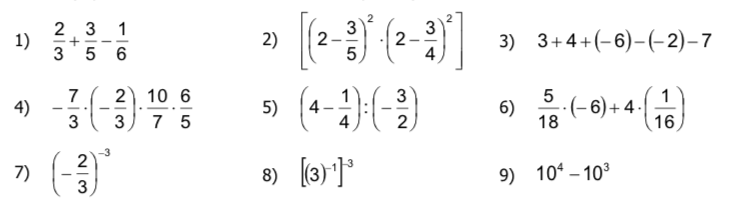
\includegraphics[scale=0.6]{test-form-1}
%
%}
\begin{minipage}{\linewidth}
	\begin{multicols}{2}
		\begin{parts}
			\part
			\exonly{$\frac{3}{3}+\frac{3}{5}-\frac{1}{6}$ }
			\solonly{$\frac{11}{10}$ }
			
			\part
			\exonly{ $\left[ \left( 2-\frac{3}{5}\right) ^2 \cdot \left( 2-\frac{3}{4}\right) ^2 \right] $  }
			\solonly{$\frac{49}{16}$ }
			
			\part
			\exonly{$3+4+(-6)-(-2)-7$ }
			\solonly{$-4$ }
			
			\part
			\exonly{$-\frac{7}{3} \cdot \left( -\frac{2}{3}\right) \cdot \frac{10}{7} \cdot \frac{6}{5} $ }
			\solonly{$\frac{8}{3}$ }
			
			\part
			\exonly{$\left( 4-\frac{1}{4}\right) \div \left( -\frac{3}{2}\right) $ }
			\solonly{$-\frac{5}{2}$ }
			
			\part
			\exonly{$\frac{15}{18}\cdot\left( -6 \right) +4\cdot \left( \frac{1}{16}\right) $ }
			\solonly{$-\frac{17}{12}$ }
			
			\part
			\exonly{$\left( -\frac{2}{3}\right) ^{-3}$ }
			\solonly{$-\frac{27}{8}$ }
			
			\part
			\exonly{$\left[ \left( 3\right) ^{-1}\right] ^{-3}$ }
			\solonly{$27$ }
			
			\part
			\exonly{$10^4-10^3$ }
			\solonly{$9000$ }
		\end{parts}
	\end{multicols}
\end{minipage}

%\solonly{
%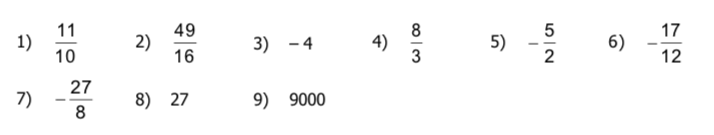
\includegraphics[scale=0.6]{test-form-1-sol}
%}

%\exnewpage

\begin{minipage}{\textwidth}	
	\question
	\exonly{Calcola senza aiutarti con la calcolatrice:}
		
	\begin{minipage}{\linewidth}
		\begin{multicols}{2}
			\begin{parts}
				
				\part 
				\exonly{$ x - 2x + 3x - 4x + 5x - 6x =$ }
				\solonly{$ -3x$ }
				
				\part 
				\exonly{$ a^2 + 2a -3a^2 +a = $ }
				\solonly{$-2a^2+3a$ }
				
				\part
				\exonly{$ a^2 \cdot a^3 = $ }
				\solonly{$a^5$ }
				\part 
				\exonly{$ \left(a^2\right)^2 + a\cdot a^3 - \left(a^6\right)^{-2} =$ }
				\solonly{$\dfrac{2a^{16}-1}{a^{12}}$ }
				
				\part 
				\exonly{$ x^{-2} \cdot \left(x^2\right)^3 = $ }
				\solonly{$x^4$ }
				
				\part 
				\exonly{$ \dfrac{9 \cdot a^2 \cdot b^3 }{3 \cdot a^{-2} \cdot b^5} = $ }
				\solonly{$\dfrac{3a^4}{b^2}$ }
				
				\part 
				\exonly{$ \dfrac{2 \cdot a^3 \cdot b^2 }{3 \cdot a \cdot b^4} \cdot \dfrac{a+b}{a}  = $ }
				\solonly{$\dfrac{2a^2+2ab}{3b^2}$ }
				
				\part 
				\exonly{$ a\left(a(a^{-1}+1) + a(a-1)\right) =$ }
				\solonly{$ a^3+a$ }
			\end{parts}
			
		\end{multicols}
		
\end{minipage}
\end{minipage}


\end{questions}

\subsection{Notazione scientifica}
\begin{questions}

\question
\exonly{Esprimi la tua altezza in notazione scientifica}
\solonly{Esempio con \SI{178}{\centi\metre} }

	\begin{multicols}{2}
		\begin{parts}
			\part 
			\exonly{in metri }
			\solonly{ \SI{1.78}{\metre} }
			\part 
			\exonly{in centimetri }
			\solonly{\SI{1.78e2}{\centi\metre} }
			\part 
			\exonly{in millimetri }
			\solonly{\SI{1.78e3}{\milli\metre} }
			\part 
			\exonly{in chilometri }
			\solonly{\SI{1.78e-3}{\kilo\metre} } 
			\part 
			\exonly{in pollici ($\SI{1}{in}=\SI{2.54}{cm}$) }
			\solonly{\SI{7.01e1}{in} }
			\part 
			\exonly{in piedi ($\SI{1}{ft}=\SI{12}{in}$) }
			\solonly{\SI{5.84}{ft} }
		\end{parts}
	\end{multicols}


\question
\exonly{Calcola senza aiutarti con la calcolatrice:}

	\begin{parts}
		\part 
		\exonly{$\num{2e3} + \num{5e2} +\num{3e1}=$ }
		\solonly{\num{2530}=\num{2.53e3} }
		\part
		\exonly{ $\num{3e3} + \num{5e-2} +\num{2e-1} + \num{6e1} + \num{4e0} + \num{9e2} + 7 \times 10^0=$ }
		\solonly{\num{3971.25} }
		
		\part 
		\exonly{$ \num{12e3} \times \num{2e-3} \times \num{3e-6} =$ }
		\solonly{\num{72e-6}=\num{7.2e-5} }
		
		\part 
		\exonly{$ \dfrac{\num{12e3}+ 500}{\num{5e6}} = $ }
		\solonly{ \num{2.5e-3}  }
		
		\part 
		\exonly{$ \dfrac{\num{2e-2} \times\num{3e1} \times\num{4e2}}{\num{4e2} \times\num{6e-3} \times\num{2e1}} =$ }
		\solonly{ \num{5}}
		
	\end{parts}

\question
\exonly{ Calcolare le seguenti espressioni ed esprimere il risultato in notazione scientifica }

\begin{minipage}{\linewidth}
	\begin{multicols}{2}
		\begin{parts}
			\part
			\exonly{ $\num{0.5e-1 }$ }
			\solonly{$ \num{5e-2}$ }
			
			\part
			\exonly{ $\num{-6.5e-5} -\num{3.5e-7} $ }
			\solonly{$-\num{6.535e-5} $ }
			
			\part
			\exonly{$\left(3 \cdot 10^{-2}\right)\left(4 \cdot 10^{-1}\right)$ }
			\solonly{ $\num{1.2e-2}$ }
			
			\part
			\exonly{$8^{2} \cdot 10^{-2}$ }
			\solonly{$\num{6.4e-1} $ }
			
			\part
			\exonly{ $200 \cdot 10^{4}$ }
			\solonly{$\num{2e6}$ }
			
			\part
			\exonly{$\left(5 \cdot 10^{-4}\right)\left(0,7 \cdot 10^{-8}\right)$ }
			\solonly{$\num{3.5e-12} $ }
			
			\part
			\exonly{$\left(7 \cdot 10^{-7}\right)^{2}$ }
			\solonly{$\num{4.9e-13}$ }
			
			\part
			\exonly{ $\left(3^{2} \cdot 10^{-6}\right)^{2} \cdot 10$ }
			\solonly{$ \num{8.1e-10} $ }
			
			\part
			\exonly{$10^{4}-10^{3}$ }
			\solonly{$\num{9e3}$ }
			
			\part
			\exonly{ $\left(0,4 \cdot 10^{-4}\right)(0,8) \cdot 10^{-4}$}
			\solonly{$\num{3.2e-9}$ }
			
			\part
			\exonly{$10^{5}-10^{-5}$ }
			\solonly{$\num{9.999999999e4}$ }
			
			\part
			\exonly{$\frac{\left(4^{2}\right)^{-2} \cdot 10^{-3}}{4^{-2} \cdot 10^{-8}}$ }
			\solonly{ $\num{6.25e3}$ }
			
			\part
			\exonly{$-\num{4.2e-3}+\num{4.2e5}$ }
			\solonly{$\num{4.199999958e5} $ }
		\end{parts}
	\end{multicols}
\end{minipage}

\question
\exonly{Calcola ed esprimi il risalutato tenendo conto delle cifre significative delle misure:}

\begin{minipage}{\linewidth}
	\begin{multicols}{2}
		\begin{parts}
			\part 
			\exonly{$ \SI{5.3}{cm} - \SI{3.2}{mm} = $  }
			\solonly{\SI{50}{\milli\metre}=\SI{5.0}{\centi\metre} }
			\part 
			\exonly{$ \SI{43.5}{cm} \cdot \SI{9.3}{mm} = $  }
			\solonly{\SI{4.0e1}{\square\centi\metre}=\SI{4.0e3}{\square\milli\metre} }
			\part
			\exonly{ $ \SI{9.2}{cm^2} + \SI{123}{mm^2} = $  }
			\solonly{ \SI{1.0e3}{\square\milli\metre} }
			\part
			\exonly{ $ \dfrac{\SI{430}{mm^2}}{\SI{3.2}{cm}} = $ }
			\solonly{$\SI{1.3e1}{mm^2}$ }
			\part 
			\exonly{$ \SI{3.2}{k\ohm} \cdot \SI{15}{mA} = $ }
			\solonly{$\SI{48}{V}$ }
			\part 
			\exonly{$ \dfrac{\SI{12}{V}}{\SI{60}{mA}} = $ }
			\solonly{\SI{2.0e2}{\ohm} }
		\end{parts}
	\end{multicols}
\end{minipage}

\question
\exonly{
	Esprimi le seguenti frazioni in notazione scientifica e tecnica tendendo conto delle cifre significative }

\begin{minipage}{\linewidth}
	\begin{multicols}{2}
		\begin{parts}
			\setlength\itemsep{1em}
			\part 
			\exonly{$\frac{5}{8}$ }
			\solonly{\num{6e-1} \\ \num{600e-3} }
			\part 
			\exonly{$\frac{724}{5}$ }
			\solonly{\solonly{\num{1e2} \\ \num{100e0} } }
			\part 
			\exonly{$\frac{11562}{470000}$ }
			\solonly{\num{2.5e-2} \\ \num{25e-3} } 
			
			\part 
			\exonly{$\frac{123456}{7}$ }
			\solonly{ \num{2e4} \\ \num{20e3}  }
			
			\part
			\exonly{ $\frac{12}{16500}$= }
			\solonly{\num{7.3e-3} \\ \num{7.3e-3}  }
			
			\part 
			\exonly{$\frac{146}{2420}$= }
			\solonly{\num{6.03e-2} \\ \num{60.3e-3}  }
		\end{parts}
	\end{multicols}
\end{minipage}


\end{questions}
\section{Monomi e polinomi}
\subsection{Effettuare, semplificare, ridurre}
\begin{questions}
	
	
	\question
	\begin{parts}
		\part
		
		\exonly{
			$\frac{2}{7} a^{5} \cdot \frac{21}{8} a^{4}=$
		}
		\solonly{
			$\frac{3}{4} a^{9}=\frac{3 a^{9}}{4}$
		}
		
		\part
		\exonly{$\frac{2 x}{9} \cdot\left(\frac{-6 a^{2}}{7 x}\right) \cdot \frac{28 x}{3 a}=$}
		\solonly{$-\frac{16}{9} ax=-\frac{16 ax}{9}$}
		
		\part
		\exonly{$\frac{3 x}{5} \cdot \frac{10 a^{3}}{x^{3}} \cdot\left(-\frac{3 x}{2 a}\right)=$}
		\solonly{ $-\frac{9 a^{2}}{x}$}
	\end{parts}
	
	
	\question
\begin{minipage}{\linewidth}
	\begin{multicols}{2}
	\begin{parts}
		\part
		\exonly{$x+x+y $ }
		\solonly{$2x+y$}
		\part
		\exonly{$ 2 x+5 y+3 x+y $} 
		\solonly{$5 x+6 y$}
		\part
		\exonly{$  7 x+9 x-10 y-20 y$}
		\solonly{$16 x-30 y$}
		\part
		\exonly{ $5 x-9 y+y-6 x $ }
		\solonly{$-x-8 y$}
		\part
		\exonly{$ 5 x^{2}+9 y^{2}-4 y^{2}+x^{2}$ }
		\solonly{$6x^{2}+5 y^{2}$}
		\part
		\exonly{$  4 x y-y^{2}+y^{2}-4 x y$}
		\solonly{$0$}
		\part
		\exonly{$ 5 x-(x+3 x) $ }
		\solonly{$x$}
		
		\part
		\exonly{$-y-(5 y-9) $ }
		\solonly{$-6 y+9$}
		
		\part
		\exonly{$ -5 x-(1-5 x)$}
		\solonly{$-1$}
		
		\part
		
		\exonly{$ 16 x-(-16 x-1)$ }
		\solonly{$32 x+1$}
		
		\part
		\exonly{$ (5 x+y)-(5 x+y)$}
		\solonly{$0$}
		
		
		\part
		\exonly{$(5 x+3 y)-(7 x+3 y)$}
		\solonly{$-2 x$}
	\end{parts}
\end{multicols}
\end{minipage}
	
	\question
	\begin{parts}
		\part
		\exonly{$x \cdot\left(x^{2}+2 x-1\right) $}
		\solonly{$x^{3}+2 x^{2}-x$}
		
		\part
		\exonly{$2y \cdot(2 x+5) \quad$}
		\solonly{$ 4x y+10 y$}
		\part
		\exonly{$3x y \cdot(5 z-3)$}
		\solonly{$15 x y z-9 x y$}
		\part
		\exonly{ $(-3 z+8) \cdot 2+x^{2}$}
		\solonly{$x^2-6z+16$}
		\part
		\exonly{$-x^{2} \cdot\left(2 x+5 x^{2}-x^{2}-x^{3}\right)-2 x \cdot\left(3 x^{2}-5 z^{2}+1\right)$}
		\solonly{$x^{5}-4 x^{4}-8 x^{3}+10xz^2-2x$}
	\end{parts}
	
	
	\question
%TODO : convert in LaTeX
		\exonly{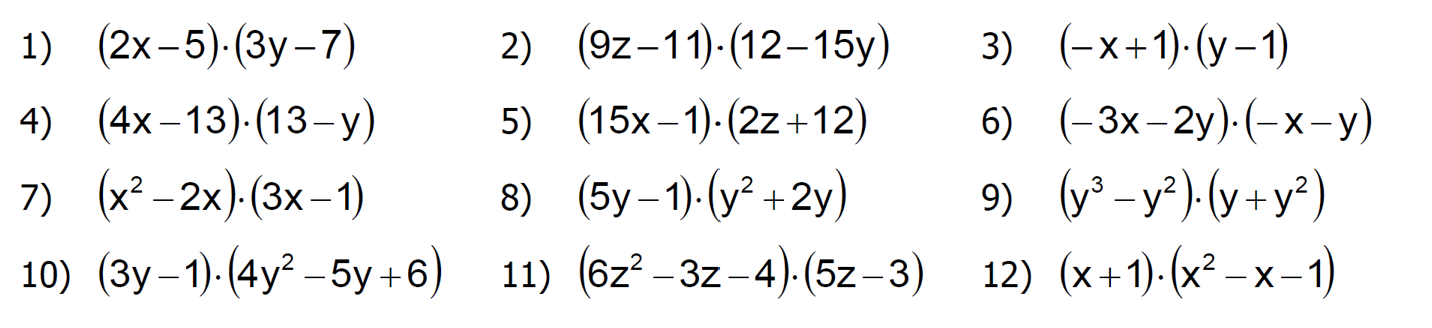
\includegraphics[scale=0.6]{molt-poli-1-25} }
		\solonly{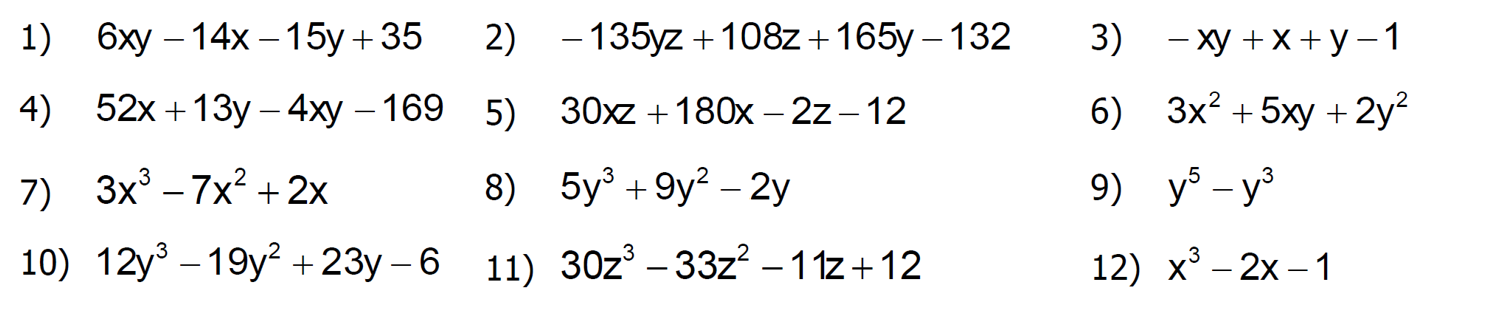
\includegraphics[scale=0.6]{molt-poli-1-25-sol} }

	\question
%TODO : convert in LaTeX
	\exonly{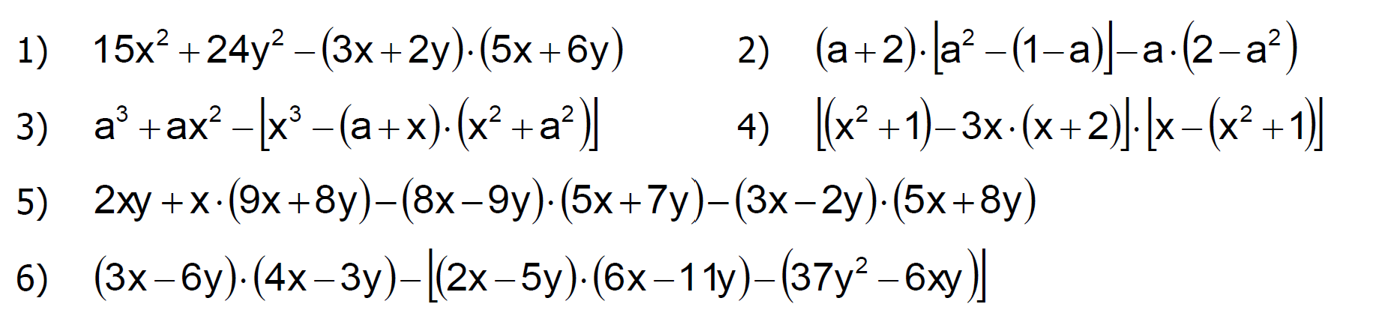
\includegraphics[scale=0.6]{molt-poli-1-26} }
	\solonly{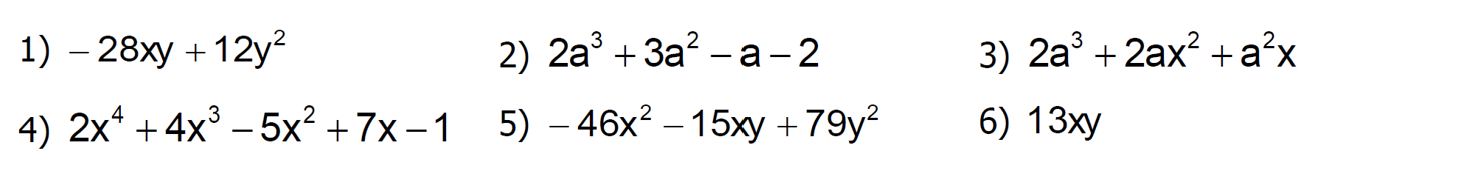
\includegraphics[scale=0.6]{molt-poli-1-26-sol} }

	\question
%TODO : convert in LaTeX
	\exonly{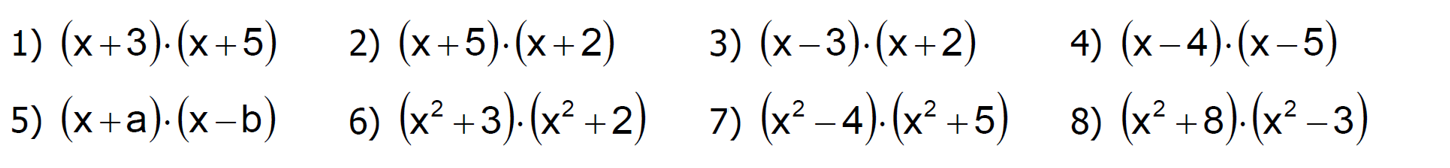
\includegraphics[scale=0.6]{molt-poli-1-27} }
	\solonly{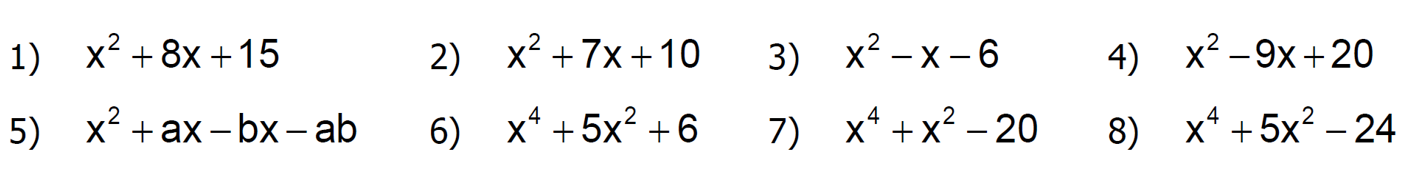
\includegraphics[scale=0.6]{molt-poli-1-27-sol} }
	
	\question

	\begin{parts}
		\part \exonly{$\dfrac{2}{5}x^2+ \dfrac{1}{4}x-2x+\dfrac{x^2}{10}=$}
		\solonly{$\dfrac{x^2}{2} - \dfrac{7}{4}x$}
		
		\part
		\exonly{$\dfrac{2}{3}\left( \dfrac{6x^2}{5}+12 \right) - \dfrac{4x}{3}\left(\dfrac{x^3}{2}-1\right)=$}
		\solonly{$-\dfrac{2x^4}{3}+\dfrac{4x^2}{5}+\dfrac{4x}{3}+8$}
		
		
		
		\part 
		\exonly{$3x- \dfrac{2}{3}x^2+ \dfrac{1}{12}x^2 + \dfrac{1}{2}x=$}
		\solonly{$-\dfrac{7x^2}{12} +\dfrac{7}{2}x$}
		
		\part
		\exonly{$\dfrac{5}{12}x + \dfrac{x}{6}-\dfrac{x}{3}+ \dfrac{1}{2}x=$}  \solonly{$\dfrac{3x}{4}$}
		
		\part
		
		\exonly{$\dfrac{1}{2}\left( 3x^3-5\right)-\dfrac{x}{3}\left(3x^3-6\right)+2x^2\left(\dfrac{x^2}{2}-\dfrac{5x}{4}-1\right)+ \dfrac{1}{2}=$ }
		\solonly{$-x^3-2x^2+2x-2 $}
	\end{parts}

	
	
\end{questions}

\newpage
\subsection{Fattorizzazione}

\begin{questions}
	
	\question 
	\exonly{Fattorizzare in $\Z[x]$ }
	
	\begin{minipage}{\linewidth}
		\begin{multicols}{2}
	\begin{parts}
		\part \exonly{$6 a+9$ } \solonly{$3(2 a+3)$ }
		\part \exonly{$15 t-10$ } \solonly{$5(3 t-2)$ }
		\part \exonly{$3 s^{2}+6 s$ } \solonly{$3 s(s+2)$ }
		\part \exonly{$12 x+16$ } \solonly{$4(3 x+4)$ }
		\part \exonly{$27 p+81$ } \solonly{$27(p+3)$ }
		\part \exonly{$18 a^{2} b^{2}-15 a^{2} b$ }  \solonly{$3 a^{2} b(6 b-5)$ }
		\part \exonly{$9 x-12$ } \solonly{$3(3 x-4)$ }
		\part \exonly{$x^{3}-x^{2}$ } \solonly{$x^{2}(x-1)$ }
		\part \exonly{$3 a^{3} b^{2}-6 a^{2} b$ } \solonly{$3 a^{2} b(a b-2)$ }
	\end{parts}
\end{multicols}
\end{minipage}

 \question \exonly{Fattorizzare  in $\Z[x]$ }
 
 	
 \begin{minipage}{\linewidth}
 	\begin{multicols}{2}
 \begin{parts}
 	\part \exonly{$x(y+3)+4(y+3)$ } \solonly{$(y+3)(x+4)$ }
  \part	\exonly{$x^{2}(2 t-1)+3(2 t-1)$ } \solonly{$(2 t-1)\left(x^{2}+3\right)$ }
  \part \exonly{$n(m-2)-(m-2)$ } \solonly{$(m-2)(n-1)$ }
  \part\exonly{$a^{2}(b+1)-a(b+1)$ } 
  \solonly{$a(b+1)(a-1)$ }
  \part \exonly{ $-2 p(q-1)+4(q-1)$  }
  \solonly{$(q-1)(-2 p+4)$ }
 \end{parts}
\end{multicols}
\end{minipage}


	\question \exonly{Fattorizzare in $\Z[x]$ }
	
%SRC : Favre es 3.3 pg 24 colonna 1
\begin{minipage}{\linewidth}
	\begin{multicols}{2}
		\begin{parts}
			\part
			\exonly{$a^{2}-9$ } \solonly{$(a-3)(a+3)$ }
			
		\part
		\exonly{$b^{2}-4 a^{2}$ } \solonly{$(b-2 a)(b+2 a)$ }
		\part
		\exonly{$x^{2}-6 x+9$ }	\solonly{ $(x-3)^{2}$ }
		
		\part
		\exonly{$1-x^{2}$ } \solonly{$(1-x)(1+x)$ }
		\part
		\exonly{$16 a^{2}-x^{2} y^{2}$ } \solonly{$(4 a-x y)(4 a+x y)$  }
		
		\part \exonly{$1+2 x^{2}+x^{4}$ } \solonly{$\left(x^{2}+1\right)^{2}$ }
		
		\part \exonly{$-144+b^{2} c^{2}$ } \solonly{$(b c-12)(b c+12)$ }
		\part \exonly{$a^{2}-9 b^{2} c^{4}$ } \solonly{$\left(a-3 b c^{2}\right)\left(a+3 b c^{2}\right)$ }
		
		\part
		\exonly{$9 x^{4}+16 y^{2}+24 x^{2} y$ }
		\solonly{ $\left(3 x^{2}+4 y\right)^{2}$ }
		
		\part
		\exonly{$x^4-81 $}
		\solonly{$(x-3)(x+3)(x^2+9)$ }
	\end{parts}
\end{multicols}
\end{minipage}


	\question \exonly{Fattorizzare in $\Z[x]$ }
	
	\begin{minipage}{\linewidth}
		\begin{multicols}{2}
	\begin{parts}
	
	\part 
	\exonly{$x^2 -6x-40$ }
	\solonly{$(x+4)(x-10)$ }
	
	
	\part 
	\exonly{$x^2 -13x+40$ }
	\solonly{$(x-5)(x-8)$ }
	
	\part
	\exonly{$x^2 +6x -55$ }
	\solonly{$(x-5)(x+11) $ }
	
	\part
	\exonly{$x^2 +7x -18$ }
	\solonly{$(x-2)(x+9)$ }

	
	
	\part
	\exonly{$x^2 -11x +28$ }
	 \solonly{$ (x-7)(x-4)$ }
	
	\part
	\exonly{$x^2 +7x +10$ }
	\solonly{$(x+5)(x+2)$ }

	
	\part
	\exonly{$x^2 -2x -48$ }
	\solonly{$(x+6)(x-8) $ }

	
	\part
	\exonly{$x^2 +2x-8$ }
	\solonly{$(x+4)(x-2) $ }

	
	\part
	\exonly{$x^2 +2x -3$ }
	\solonly{$(x+3)(x-1)$ }

	
	\part
	\exonly{$x^2 -12x +35$ }
	\solonly{$(x-5)(x-7)$ }

	
	\part
	\exonly{$x^2 +5x-36$ }
	\solonly{$(x-4)(x+9)$ }

	
	\part
	\exonly{$x^2 -7x+15$ }
	\solonly{Irriducibile in $\Z[x]$ }

	
	\part
	\exonly{$x^2 +23x +120$ }
	\solonly{$(x+15)(x+8)$ }

	
	\part
	\exonly{$x^2 -23x +132$ }
	\solonly{$(x-12)(x-11)$ }

	
	\part
	\exonly{$x^2+x-56$ }
	\solonly{$(x-7)(x+8)$ }

	
\end{parts}
\end{multicols}
\end{minipage}

% \exnewpage
% \solnewpage
\question
\exonly{Fattorizzare in $\Z[x]$  (valutazione formativa 1) }
 \solonly{ 
	I vari simboli ($\star$, \dots , $\Diamond$$\Diamond$$\Diamond$) permettono di raggruppare gli esercizi in funzione del metodo di fattorizzazione  da padroneggiare.
	
	$\star$: Messa in evidenza del MCD \\
	$\star\star$: Prodotti notevoli di grado 2 \\
%	$\star\star\star$: Prodotti notevoli di grado 3 \\
	$\Diamond$: Trinomio \\
%	$\Diamond\Diamond$: Raggruppamento\\
	$\Diamond\Diamond\Diamond$: Messa in evidenza e metodi vari
}

	\begin{minipage}{\linewidth}
	\begin{multicols}{2}
\begin{parts}
\part
\exonly{ $15x^{3} y^{4} +20x^{5} y^{4} -30x^{2} y^{3} =$}
\solonly{$\star$ $5x^{2} y^{3} \left(3xy+4x^{3} y-6\right)$}

\part  
\exonly{$64x^{2} +16x+1=$}
\solonly{$\star$$\star$ $\left(8x+1\right)^{2} $}

\part  
\exonly{$3x^{2} -18x-120=$}
\solonly{$\Diamond$ $3\left(x-10\right)\left(x+4\right)$}






\part  
\exonly{$49x^{2} -1=$}
\solonly{  $\star$$\star$ $\left(7x+1\right)\left(7x-1\right)$}

\part  
\exonly{$x^{2} -13x+40=$}
\solonly{  $\Diamond$ $\left(x-8\right)\left(x-5\right)$}




\part  
\exonly{$3x^{4} +60x^{3} +300x^{2} =$}
\solonly{  $\Diamond$$\Diamond$$\Diamond$ $3x^{2} \left(x+10\right)^{2} $}


			\part  
\exonly{$9x^{2} -25y^{2} =$}
\solonly{  $\star$$\star$ $\left(3x+5y\right)\left(3x-5y\right)$}


			\part  
\exonly{$27x^{3} -75x=$}
\solonly{  $\Diamond$$\Diamond$$\Diamond$ $3x\left(3x+5\right)\left(3x-5\right)$}



\part  
\exonly{$6x^{2} y^{3} +18x^{3} y^{4} -24x^{4} y^{3} =$}
\solonly{  $\star$ $6x^{2} y^{3} \left(1+3xy-4x^{2} \right)$}



\part
\exonly{$x^2-9x -20$ }
\solonly{ $\Diamond$ Irriducibile in $\Z[x]$ }




\part  
\exonly{$x^{2} +6x-55=$}
\solonly{  $\Diamond$ $\left(x+11\right)\left(x-5\right)$}



			\part  
\exonly{$121x^{2} -25=$}
\solonly{  $\star$$\star$ $\left(11x+5\right)\left(11x-5\right)$}


\part  
\exonly{$27x^{3} -12x=$}
\solonly{  $\Diamond$$\Diamond$$\Diamond$ $3x\left(3x+2\right)\left(3x-2\right)$}


		
		
\part  
\exonly{$x^{2} +7x-18=$}
\solonly{  $\Diamond$ $\left(x+9\right)\left(x-2\right)$}



\part  
\exonly{$12a^{4} b^{3} -6a^{2} b^{4} +24a^{3} b^{3} =$}
\solonly{  $\star$ $6a^{2} b^{3} \left(2a^{2} -b+4a\right)$}



	
	
	
\end{parts}

\end{multicols}
\end{minipage}




\question \exonly{Fattorizzare in $\Z[x]$ }

\begin{minipage}{\linewidth}
	\begin{multicols}{2}
		\begin{parts}
			\part
			\exonly{$2ax-6bx+ay-3by$ }
			\solonly{ $(a-3 b) (2 x+y) $}
			
			\part
			\exonly{$2ay^2-axy+6xy-3x^2$ }
			\solonly{$(2 y-x) (a y+3 x)$ }
			
			\part
			\exonly{$3x^3+3x^2-27x-27= $ }
			\solonly{$3 (x+1) (x-3) (x+3)$ }
			
			\part
			\exonly{$5x^3+10x^2-20x-40 $ }
			\solonly{$5 (x-2) (x+2)^2 $ }
			
			\part
			\exonly{	$x^4+2x^3-x-2$ }
			\solonly{$(x+2) (x-1) (x^2+x+1) $ }
			\part
			\exonly{$3 x^3 - 2 x^2 + 6 x - 4$ }
			\solonly{$(x^2+2)(3x-2) $ }
			
			
			\part
			\exonly{$4 x^3 + 8 x^2 - x - 2$ }
			\solonly{$(x+2)(2x-1)(2x+1)$ }
			
		\end{parts}
	\end{multicols}
\end{minipage}


% \solnewpage
\question
\exonly{Fattorizzare in $\Z[x]$  (valutazione formativa 2) }
\solonly{ 
	I vari simboli ($\star$, \dots , $\Diamond$$\Diamond$$\Diamond$) permettono di raggruppare gli esercizi in funzione del metodo di fattorizzazione  da padroneggiare.
	
	$\star$: Messa in evidenza del MCD \\
	$\star\star$: Prodotti notevoli di grado 2 \\
	$\star\star\star$: Prodotti notevoli di grado 3 \\
	$\Diamond$: Trinomio \\
	$\Diamond\Diamond$: Raggruppamento\\
	$\Diamond\Diamond\Diamond$: Messa in evidenza e metodi vari
}

\begin{minipage}{\linewidth}
	\begin{multicols}{2}
		\begin{parts}

			\part  
			\exonly{$27a^{3} +343=$}
			\solonly{$\star$$\star$$\star$ $\left(3a+7\right)\left(9a^{2} -21a+49\right)$}
			
			
			\part  
			\exonly{$36x^{2} -60x+25=$}
			\solonly{  $\star$$\star$ $\left(6x-5\right)^{2} $}
			
			
			\part  
			\exonly{$25x^{2} +40x+16=$}
			\solonly{  $\star$$\star$ $\left(5x+4\right)^{2} $}
			
			
			\part  
			\exonly{$8a^{2} -6ab+20ad-15bd=$}
			\solonly{  $\Diamond$$\Diamond$ $\left(4a-3b\right)\left(2a+5d\right)$}
			
			\part  
			\exonly{$125a^{3} -216=$ }
			\solonly{  $\star$$\star$$\star$ $\left(5a-6\right)\left(25a^{2} +30a+36\right)$} 		
			

			
			\part  
			\exonly{$216a^{3} -125=$ }
			\solonly{  $\star$$\star$$\star$ $\left(6a-5\right)\left(36a^{2} +30a+25\right)$} 
			
			

			
			
		\part  
			\exonly{$15x^{2} -10xy-9xz+6yz=$}
			\solonly{$\Diamond$$\Diamond$ $\left(5x-3z\right)\left(3x-2y\right)$}
			
			\part  
			\exonly{$8x^{3} -729=$}
			\solonly{  $\star$$\star$$\star$ $\left(2x-9\right)\left(4x^{2} +18x+81\right)$}
			
			\part  
			\exonly{$6a^{2} +15a-8ab-20b=$}
			\solonly{  $\Diamond$$\Diamond$ $\left(3a-4b\right)\left(2a+5\right)$}
			
			
			\part  
			\exonly{$15a^{3} b^{5} -10a^{2} b^{4} +20a^{3} b=$}
			\solonly{  $\star$ $5a^{2} b\left(3ab^{4} -2b^{3} +4a\right)$}
			
			

			
			
			\part  
			\exonly{$8a^{2} -6ab+20ad-15bd=$}
			\solonly{  $\Diamond$$\Diamond$ $\left(4a-3b\right)\left(2a+5d\right)$}
			
			
			\part  
			\exonly{$4x^{3} -32x^{2} +64x=$}
			\solonly{  $\Diamond$$\Diamond$$\Diamond$ $4x\left(x-4\right)^{2} $}
			
			
			\part  
			\exonly{$x^{2} -6x-40=$}
			\solonly{  $\Diamond$ $\left(x-10\right)\left(x+4\right)$}
			
			
			\part  
			\exonly{$27x^{3} +512=$ }
			\solonly{  $\star$$\star$$\star$ $\left(3x+8\right)\left(9x^{2} -24x+64\right)$} 
			
			
			\part  
			\exonly{$8x^{3} y^{3} +6x^{4} y^{5} -10x^{2} y^{4} =$}
			\solonly{  $\star$ $2x^{2} y^{3} \left(4x+3x^{2} y^{2} -5y\right)$}
			
			\part  
			\exonly{$8a^{2} +4ab-2ac-bc=$}
			\solonly{  $\Diamond$$\Diamond$ $\left(2a+b\right)\left(4a-c\right)$}
			
			
			

			
			\part  
			\exonly{$8x^{2} +10xy+4xz+5yz=$}
			\solonly{  $\Diamond$$\Diamond$ $\left(2x+z\right)\left(4x+5y\right)$}
			
			\part  
			\exonly{$x^{2} -11x+28=$}
			\solonly{  $\Diamond$ $\left(x-4\right)\left(x-7\right)$}
			
			\part  
			\exonly{$12x^{4} +60x^{3} +75x^{2} =$}
			\solonly{  $\Diamond$$\Diamond$$\Diamond$ $3x^{2} \left(2x+5\right)^{2} $}
			
			\part  
			\exonly{$27x^{3} -125=$}
			\solonly{$\star$$\star$$\star$$\left(3x-5\right)\left(9x^{2} +15x+25\right)$}	
			
		
		\part
		\exonly{$15 x^2 - x - 2=$}
		\solonly{$\Diamond$  $(5x-2)(3x+1)$}
		
			
			
		\end{parts}
		
	\end{multicols}
\end{minipage}
\end{questions}


% \exnewpage
\subsection{Applicazioni della fattorizzazione: frazioni algebriche}
\begin{questions}
\question
Semplificare le seguenti frazioni algebriche

% \exonly{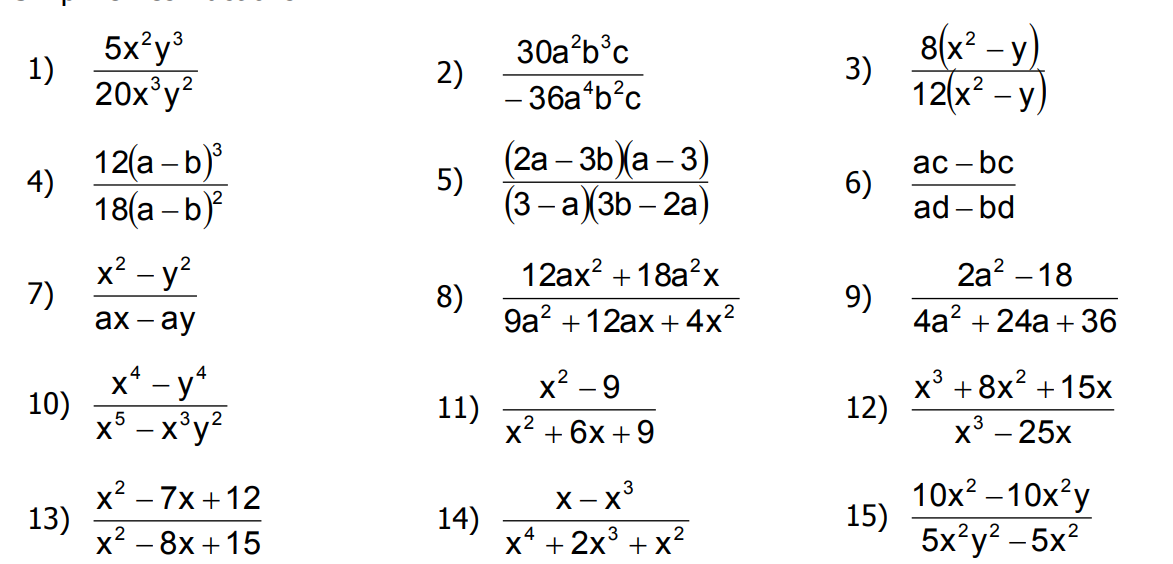
\includegraphics[scale=0.7]{frazioni-alg-4-1} }
% \solonly{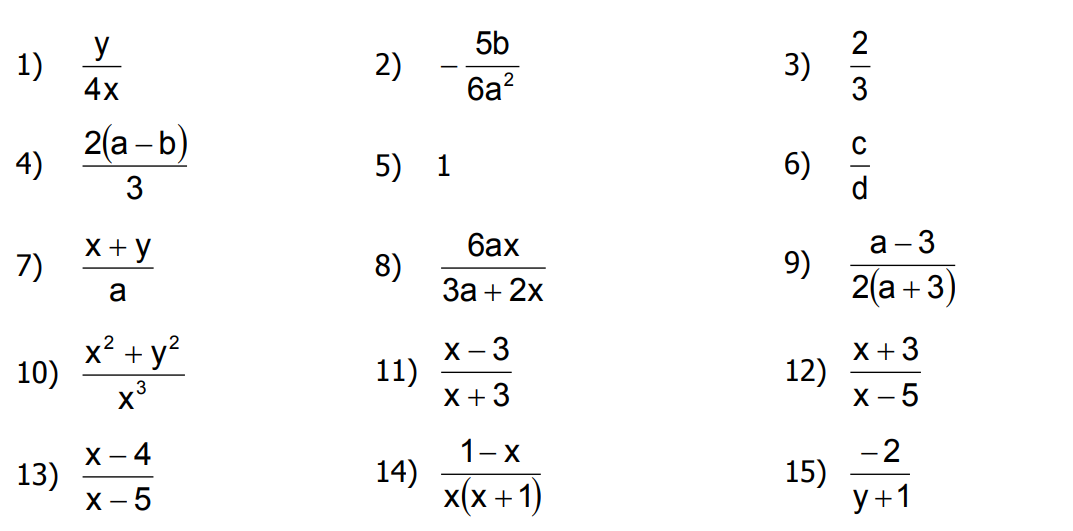
\includegraphics[scale=0.7]{frazioni-alg-4-1-sol} }
\begin{minipage}{\linewidth}
	\begin{multicols}{2}
		\begin{parts} %% Esercizio 4.1 EPAI
			\part
			\exonly{$\frac{5x^2y^3}{20x^3y^2}$}
			\solonly{$\frac{y}{4x}$} 

			\part
			\exonly{$\frac{30a^2b^3c}{-36a^4b^2c}$}
			\solonly{$-\frac{5b}{6a^2}$} 

			\part
			\exonly{$\frac{8(x^2-y)}{12(x^2-y)}$}
			\solonly{$\frac{2}{3}$} 

			\part
			\exonly{$\frac{12(a-b)^3}{18(a-b)^2}$}
			\solonly{$\frac{2(a-b)}{3}$} 

			\part
			\exonly{$\frac{(2a-3b)(a-3)}{(3-a)(3b-2a)}$}
			\solonly{$1$} 


			\part
			\exonly{$\frac{ac-bc}{ad-bd}$}
			\solonly{$\frac{c}{d}$} 

			\part
			\exonly{$\frac{x^2-y^2}{18(a-b)^2}$}
			\solonly{$\frac{x+y}{a}$} 

			\part
			\exonly{$\frac{12ax^2+18a^2x}{9a^2+12ax+4x^2}$}
			\solonly{$\frac{6ax}{3a+2x}$} 

			\part
			\exonly{$\frac{2a^2-18}{4a^2+24a+36}$}
			\solonly{$\frac{a-3}{2(a+3)}$} 

			\part
			\exonly{$\frac{x^4-y^4}{x^5-x^3y^2}$}
			\solonly{$\frac{x^2+y^2}{x^3}$} 

			\part
			\exonly{$\frac{x^2-9}{x^2+6x+9}$}
			\solonly{$\frac{x-3}{x+3}$} 

			\part
			\exonly{$\frac{x^3+8x^2+15x}{x^3-25x}$}
			\solonly{$\frac{x+3}{x-5}$} 

			\part
			\exonly{$\frac{x^2-7x+12}{x^2-8x+15}$}
			\solonly{$\frac{x-4}{x-5}$} 

			\part
			\exonly{$\frac{x-x^3}{x^4+2x^3+x^2}$}
			\solonly{$\frac{1-x}{x(x+1)}$} 

			\part
			\exonly{$\frac{10x^2-10x^2y}{5x^2y^2-5x^2}$}
			\solonly{$\frac{-2}{y+1}$} 

			
			
		\end{parts}
	\end{multicols}
\end{minipage}	


\question
Effettuare e semplificare

% \exonly{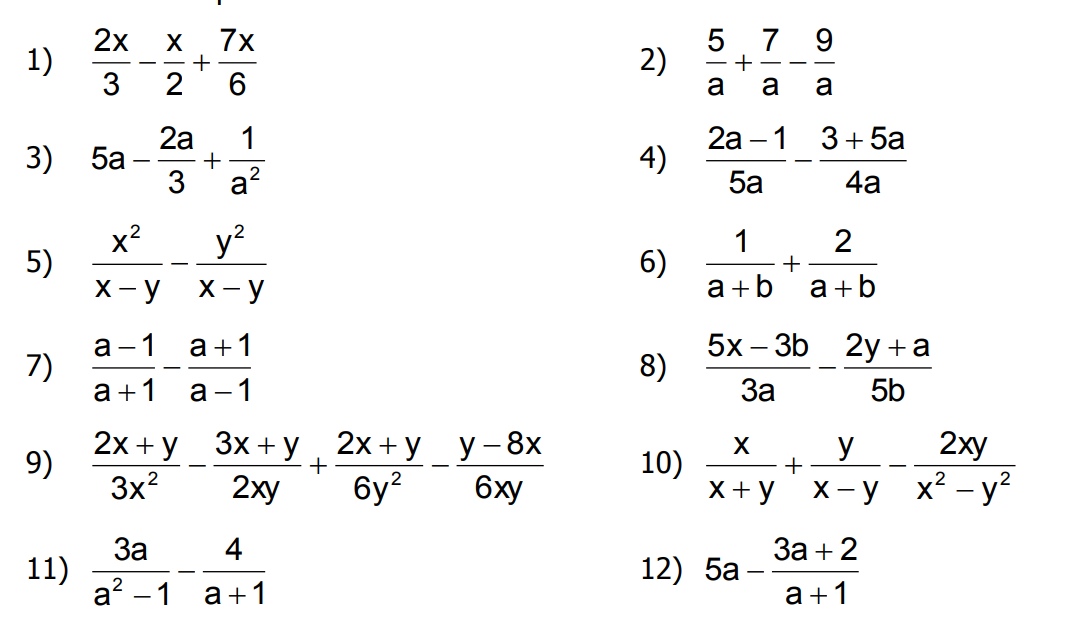
\includegraphics[scale=0.7]{frazioni-alg-4-2} }
% \solonly{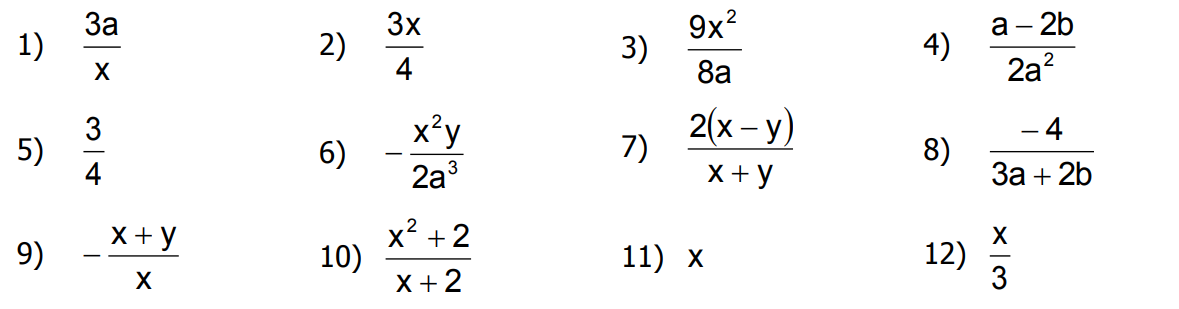
\includegraphics[scale=0.7]{frazioni-alg-4-2-sol} }


\begin{minipage}{\linewidth}
	\begin{multicols}{2}
		\begin{parts} %% Esercizio 4.4 EPAI
			\part
			\exonly{$\frac{2x}{3}-\frac{x}{2}+\frac{7x}{6}$}
			\solonly{$\frac{4x}{3}$} 

			\part
			\exonly{$\frac{5}{a}+\frac{7}{a}-\frac{9}{a}$}
			\solonly{$\frac{3}{a}$} 

			\part
			\exonly{$5a-\frac{2a}{3}+\frac{1}{a^2}$}
			\solonly{$\frac{13a^3+3}{3a^2}$} 

			\part
			\exonly{$\frac{2 a-1}{5 a}-\frac{3+5 a}{4 a}$}
			\solonly{$-\frac{17 a+19}{20 a}$} 

			\part
			\exonly{$\frac{x^2}{x-y}-\frac{y^2}{x-y}$}
			\solonly{$x+y$} 

			\part
			\exonly{$\frac{1}{a+b}+\frac{2}{a+b}$}
			\solonly{$\frac{3}{a+b}$} 

			\part
			\exonly{$\frac{a-1}{a+1}-\frac{a+1}{a-1}$}
			\solonly{$\frac{-4a}{(a+1)(a-2)}$} 

			\part
			\exonly{$\frac{5 x-3 b}{3 a}-\frac{2 y+a}{5 b}$}
			\solonly{$\frac{25bx-15b^2-6ay-3a^2}{15ab}$} 

			\part
			\exonly{$\frac{2 x+y}{3 x^2}-\frac{3 x+y}{2 x y}+\frac{2 x+y}{6 y^2}-\frac{y-8 x}{6 x y}$}
			\solonly{$\frac{x^3+y^3}{3x^2y^2}$} 

			\part
			\exonly{$\frac{x}{x+y}+\frac{y}{x-y}-\frac{2 x y}{x^2-y^2}$}
			\solonly{$\frac{x-y}{x+y}$} 

			\part
			\exonly{$\frac{3 a}{a^2-1}-\frac{4}{a+1}$}
			\solonly{$\frac{-a+4}{(a+1)(a-1)}$} 

			\part
			\exonly{$5 a-\frac{3 a+2}{a+1}$}
			\solonly{$\frac{5a^2+2a-2}{a+1}$} 
			
		\end{parts}
	\end{multicols}
\end{minipage}		

	



	
\end{questions}
\section{Modelli di primo  grado}

\subsection{Invertire formule}
\begin{questions}

	\begin{qblock}

		\question
		\exonly{Legge oraria del moto rettilineo uniforme MRU

			\begin{equation*}
				x=v \cdot t + x_0
			\end{equation*}

			\begin{center}
				\renewcommand\arraystretch{1.2}
				\begin{tabular}{lll}
					\hline
					variabile & grandezza          & unità di misura    \\
					\hline
					$x$       & posizione          & $\si{m}$           \\
					$v$       & velocità           & $\si{\frac{m}{s}}$ \\
					$t$       & tempo trascorso    & $\si{s}$           \\
					$x_o$     & posizione iniziale & $\si{m}$           \\
					\hline
				\end{tabular}
			\end{center}
		}


		\begin{parts}
			\part \exonly{Trova la formula per calcolare ogni variabile in funzione delle altre }

			$v  =  \solonly{\dfrac{x-x_0}{t} }$ \\
			$	t  = \solonly{\dfrac{x-x_0}{v} }$ \\
			$	x_0  = \solonly{x-vt}
			$




			\part \exonly{Calcola i valori mancanti nella seguente tabella }

			\bigskip

			\renewcommand\arraystretch{2.2}
			\begin{tabular}{|C{3cm}|C{3cm}|C{3cm}|C{3cm}|}
				\hline
				$x$                           & $v$                                     & $t$                       & $x_o$                      \\
				\hline
				\solonly{\SI{41.5}{\metre}  } & $\SI{3}{\frac{m}{s}}$                   & $\SI{13}{s}$              & $\SI{2.5}{m}$              \\
				%		\midrule
				$\SI{23}{km}$                 & \solonly{$\SI{5.94}{\frac{km}{h}}  $  } & $\SI{3.2}{h}$             & $\SI{4}{km}$               \\
				%		\midrule
				$\SI{173}{m}$                 & $\SI{2.7}{\frac{m}{s}}$                 & \solonly{$\SI{48.5}{s}$ } & $\SI{42}{m}$               \\
				%		\midrule
				$\SI{236}{km}$                & $\SI{123}{\frac{km}{h}}$                & $\SI{5}{h}$               & \solonly{$\SI{-379}{km}$ } \\
				%		\midrule
				$\SI{1323}{m}$                & \solonly{$\SI{21.77}{\frac{m}{min}}$ }  & $\SI{47}{min}$            & $\SI{300}{m}$              \\
				\hline
			\end{tabular}

		\end{parts}
	\end{qblock}

	\begin{qblock}
		\question
		\exonly{Resistenza di un conduttore
			\nopagebreak
			\begin{equation*}
				R=\dfrac{\rho \cdot l}{A}
			\end{equation*}
			\nopagebreak

			\begin{center}
				\renewcommand\arraystretch{1.2}
				\begin{tabular}{lll}
					\hline
					variabile & grandezza                 & unità di misura                  \\
					\hline
					$R$       & resistenza del conduttore & $\si{\ohm}$                      \\
					$\rho$    & resistività del materiale & $\si{\frac{\ohm \cdot mm^2}{m}}$ \\
					$l$       & lunghezza del conduttore  & $\si{m}$                         \\
					$A$       & sezione del conduttore    & $\si{mm^2}$                      \\
					\hline
				\end{tabular}
			\end{center}
		}


		\begin{parts}
			\part  \exonly{Trova la formula per calcolare ogni variabile in funzione delle altre }

			$\rho= \solonly{\dfrac{AR}{l} }$\\
			$l=\solonly{\dfrac{AR}{\rho} }$\\
			$A=\solonly{\dfrac{\rho l }R }$

			\nopagebreak

			\part \exonly{Calcola i valori mancanti nella seguente tabella }

			\bigskip

			\renewcommand\arraystretch{2.2}
			\begin{tabular}{|C{3cm}|C{3cm}|C{3cm}|C{3cm}|}
				\hline
				$R$                          & $\rho$                                               & $l$                            & $A$                            \\
				\hline
				\solonly{$\SI{8.75}{\ohm} $} & $\SI{0.0175}{\frac{\ohm \cdot mm^2}{m}}$             & $\SI{250}{m}$                  & $\SI{0.5}{mm^2}$               \\
				%		\midrule
				$\SI{10}{\ohm}$              & \solonly{$\SI{0.017}{\frac{\ohm \cdot mm^2}{m}}$  }  & $\SI{1.5}{km}$                 & $\SI{2.5}{mm^2}$               \\
				%		\midrule
				$\SI{152}{m\ohm}$            & $\SI{0.0287}{\frac{\ohm \cdot mm^2}{m}}$             & \solonly{$\SI{2.12}{\metre}$ } & $\SI{0.4}{mm^2}$               \\
				%		\midrule
				$\SI{0.5}{\ohm}$             & $\SI{0.0175}{\frac{\ohm \cdot mm^2}{m}}$             & $\SI{3.5}{km}$                 & \solonly{ $\SI{122.5}{mm^2}$ } \\
				%		\midrule
				$\SI{2}{\ohm}$               & \solonly{$\SI{0.0286}{\frac{\ohm \cdot mm^2}{m}}$  } & $\SI{105}{m}$                  & $\SI{1.5}{mm^2}$               \\
				\hline
			\end{tabular}

		\end{parts}
	\end{qblock}

\end{questions}

\subsection{Equazioni e sistemi di primo grado}
\begin{questions}

	\begin{qblock}
		\question

		\exonly{ Risolvi le seguenti equazioni: }
		\begin{parts}
			\setlength\itemsep{3mm}
			\item
			\exonly{$x-3=2$ }
			\solonly{$\es{5}$}

			\item \exonly{$3x=9$ } \solonly{$\es{3 }$}
			\item \exonly{$2x+3=7$ } \solonly{$\es{2 }$ }
			\item \exonly{$3x-5=7-x$ } \solonly{$\es{3 }$ }
			\item \exonly{$3x+2=5$ } \solonly{$\es{1 }$ }
			\item \exonly{$5x+3=2x-7$ } \solonly{$\es{-\frac{10}{3} }$ }
			\item \exonly{$2x+3-7x=3x-5+2x-1$ } \solonly{$\es{\frac{9}{10} }$ }
		\end{parts}
	\end{qblock}

	\begin{qblock}
		\question
		\exonly{Risolvi le seguenti equazioni: }

		\begin{parts}
			\setlength\itemsep{3mm}
			\item \exonly{$2(3x-2)+3(x-1)=4(x-1)-(3-x)$ }
			\solonly{$\es{0 }$ }

			\item \exonly{$\frac{2}{3}(5x+3)-2(\frac{1}{3}x-\frac{3}{4})=\frac{1}{2}(\frac{3}{5}-\frac{3}{7}x)$ }
			\solonly{$\es{-\frac{672}{605} }$ }

			\item \exonly{$3(x-5)+2(3-2x)=x+3-2(x-4)$ }
			\solonly{$S=\emptyset$ }

			\item \exonly{$(x+3)(x-2)=x(x+3)-3(x-4)$ }
			\solonly{$\es{18 }$ }
			\item \exonly{$2(3x-4)=4(x+1)+2(x-6)$ }
			\solonly{$S=\R$ }
		\end{parts}
	\end{qblock}

	\begin{qblock}
		\question
		\exonly{ Risolvi le seguenti equazioni nell'incognita $x$ e discuti le soluzioni in funzione del parametro $a$: }

		\begin{parts}
			\setlength\itemsep{3mm}
			\item \exonly{$2x+3-2a=3x-5+2a-1$ } \solonly{$\es{9-4a \mid a \in \R }$ }
			\item \exonly{$2(3x-2a)+3(x-a)=4(x-a)-(3a-x)$ } \solonly{$\es{0 \mid a \in \R }$ }
			\item \exonly{$3(x-5a)+2(3-2x)=x+3-2(x-4a)$ } \solonly{Se $a=\frac{3}{23}$: $S=\R$, se $a\neq\frac{3}{23}$: $S=\emptyset$ }
			\item \exonly{$(x+3)(x-a)=x(x+2a)-3(x-4)$ } \solonly{$\es{\frac{a+4}{2-a} \mid a \neq 2 }$ , se $a=2$: $S=\emptyset$ }
		\end{parts}

	\end{qblock}

	\begin{qblock}
		\question
		\exonly{Risolvere i seguenti sistemi. }


		\begin{multicols}{2}
			\begin{parts}
				\setlength\itemsep{3mm}

				\item
				\exonly{$
						\left\{
						\begin{aligned}
							x+3 & = 3x-1 \\
							x-y & = 5
						\end{aligned}
						\right. $ }
				\solonly{$\es{\left(2;-2\right)}$ }

				\item
				\exonly{ $
						\left\{
						\begin{aligned}
							2x-3  & = 4-5x \\
							3x-2y & = 2
						\end{aligned}
						\right. $ }
				\solonly{$\es{\left( 1;\frac{1}{2}\right)  }$ }

				\item
				\exonly{$
						\left\{
						\begin{aligned}
							2x-4  & = 3 \\
							-x+2y & = 5
						\end{aligned}
						\right. $ }
				\solonly{$\es{\left( \frac{7}{2};\frac{17}{4}\right) }$ }




				\item
				\exonly{$
						\left\{
						\begin{aligned}
							5x-5   & = 1  \\
							-6x+9y & = -3
						\end{aligned}
						\right. $ }

				\solonly{$\es{\left( \frac{6}{5};\frac{7}{15}\right)  }$ }
			\end{parts}
		\end{multicols}
	\end{qblock}

	\begin{qblock}
		\question
		\exonly{Risolvere i  seguenti sistemi e indicare l'insieme delle soluzioni. }
		\begin{multicols}{2}
			\begin{parts}
				\setlength\itemsep{3mm}
				\item
				\exonly{
					$\left\{
						\begin{aligned}
							3x-y  & = 2 \\
							2x-5y & = 4
						\end{aligned}
						\right. $
				}

				\solonly{
					$\es{\left( \frac{6}{13};-\frac{8}{13}\right)  }$
				}

				\item
				\exonly{$
						\left\{
						\begin{aligned}
							x+3y  & = 3  \\
							2x+4y & = -8
						\end{aligned}
						\right. $ }

				\solonly{
					$\es{\left( -18;7\right)  }$
				}
				\item \exonly{$
						\left\{
						\begin{aligned}
							2x-3y & = 1 \\
							2x-5y & = 4
						\end{aligned}
						\right. $ }

				\solonly{
					$\es{\left( -\frac{7}{4};-\frac{3}{2}\right)  }$
				}
				\item
				\exonly{$
						\left\{
						\begin{aligned}
							3x+3y & = 3  \\
							2x-3y & = -2
						\end{aligned}
						\right. $ }

				\solonly{
					$\es{\left( \frac{1}{5};\frac{4}{5}\right)  }$
				}

				\item \exonly{$
						\left\{
						\begin{aligned}
							4x-3  & = 2 \\
							2x-6y & = 4
						\end{aligned}
						\right. $ }

				\solonly{
					$\es{\left( \frac{5}{4};-\frac{1}{4}\right)  }$
				}

				\item \exonly{$
						\left\{
						\begin{aligned}
							2x+3y & = 3  \\
							6x+4y & = -3
						\end{aligned}
						\right. $ }

				\solonly{
					$\es{\left(- \frac{21}{10};\frac{12}{5}\right)  }$
				}

				\item \exonly{$
						\left\{
						\begin{aligned}
							3x-4y & = 6  \\
							2x-3y & = -8
						\end{aligned}
						\right. $ }

				\solonly{
					$\es{\left(-14;-12\right)  }$
				}
				\item \exonly{$
						\left\{
						\begin{aligned}
							4x+5y & = 3  \\
							2x+7y & = -8
						\end{aligned}
						\right. $ }

				\solonly{
					$\es{\left(\frac{61}{18};-\frac{19}{9}\right)  }$
				}



			\end{parts}
		\end{multicols}
	\end{qblock}

	\begin{qblock}

		\question
		\exonly{Risolvere i seguenti sistemi e indicare l'insieme delle soluzioni discutendo le soluzioni in funzione del parametro $a$.}

		\begin{parts}
			\item \exonly{$
					\left\{
					\begin{aligned}
						3x+5y & = -2a \\
						x+4y  & = 4
					\end{aligned}
					\right. $	 }

			\solonly{
				$\es{\left(- \frac{8a+20}{7};\frac{2a+12}{7}\right) \mid a \in \R }$
			}

			\item\exonly{ $
					\left\{
					\begin{aligned}
						2x+a\cdot y & = -6 \\
						2x-7y       & = -a
					\end{aligned}
					\right. $ }

			\solonly{
				Se $a \neq -7$: 	$\es{\left(\frac{-a^2 - 42}{2a+14}; \frac{a-6}{a+7}\right) }$  \\
				Se $a = -7$: 	$S=\emptyset $  \\
			}



		\end{parts}
	\end{qblock}

	\begin{qblock}
		\question
		\exonly{Risolvere i seguenti sistemi}

		\begin{multicols}{2}
			\begin{parts}
				\part
				\exonly{$
						\left\{
						\begin{aligned}
							x+y+z  & = 3  \\
							x-y-z  & = 4  \\
							-x+y-z & = -2
						\end{aligned}
						\right. $ }

				\solonly{$\es{\left(\frac{7}{2}; \frac{1}{2};-1\right) }$   }


				\part
				\exonly{ $
						\left\{
						\begin{aligned}
							3x-4y+z  & = 2  \\
							2x+2y-3z & = 1  \\
							3x-3y+2z & = -2
						\end{aligned}
						\right. $ }

				\solonly{$\es{\left(-1; -\frac{9}{5};-\frac{11}{5}\right) }$   }

				\part
				\exonly{ $
						\left\{
						\begin{aligned}
							2x - 3y + z & =  x -  y - z \\
							x + 2y - z  & =  2 - 3x     \\
							2x + 4y +3z & = -x +z + 1
						\end{aligned}
						\right. $ }

				\solonly{$\es{\left(\frac{11}{25}; \frac{1}{50};-\frac{1}{5}\right) }$   }

			\end{parts}
		\end{multicols}
	\end{qblock}
\end{questions}


\subsection{Funzioni e rappresentazione grafica }
\begin{questions}

	\begin{qblock}

		\question
		\exonly{Determinare la legge di assegnazione (l'equazione) delle rette) $a$, $b$, $c$, $d$ et $e$. }

		%\includegraphics[scale=1]{ex-eq-droites-rev.png}
		\exonly{
			\begin{tikzpicture}
				\begin{axis}[
						AxisDefaults,
						SmallAxisLabels,
						width=0.75\linewidth,
						domain=-6:10,
						restrict y to domain=-5:8,
						xmin=-6,xmax=10, ymin=-4, ymax=7,
					]
					\addplot[]{5*x/2+3/2} node[above left, pos=0.8] {$a$} ;
					\addplot[]{-5*x/6+7/3}node[above, pos=0.15] {$b$} ;
					\addplot[]{2}node[above, pos=0.2] {$c$} ;
					\addplot[]{7*x/3-37/3}node[ right, pos=0.8] {$d$} ;
					\addplot[]{-9*x/5+66/5}node[above right, pos=0.2] {$e$} ;
				\end{axis}
			\end{tikzpicture} }

		\solonly{


			\begin{multicols}{2}
				\begin{enumerate}[a)]
					\item $y=\frac{5}{2}x+\frac{3}{2}$
					\item $y=-\frac{5}{6}x+\frac{7}{3}$
					\item $y=2$
					\item $y=\frac{7}{3}x-\frac{37}{3}$
					\item $y=-\frac{9}{5}x+\frac{66}{5}$

				\end{enumerate}
			\end{multicols}

		}
	\end{qblock}

	\begin{qblock}
		\question
		\exonly{Determinare la legge di assegnazione (equazioni) delle rette qui sotto: }


		\exonly{\begin{tikzpicture}
				\begin{axis}[
						AxisDefaults,
						SmallAxisLabels,
						width=0.75\linewidth,
						domain=-8:10,
						restrict y to domain=-8:8,
						ymin=-6, ymax=7, %set the min and max y tick
						xmin=-8, xmax=10,  %set the min and max x tick
					]
					\addplot[black]{-5*\x/6+1} node[above,pos=0.1] {$a$};
					\addplot[black]{\x/5-4} node[above,pos=0.8] {$b$};
					\addplot[black]{\x+4} node[right,pos=0.9] {$c$};
					\addplot[black]{2*\x/5-3} node[above,pos=0.9] {$d$};
					\addplot[black]{-6*\x +6} node[right,pos=0.8] {$e$};
				\end{axis}
			\end{tikzpicture} }


		\solonly{
			\begin{multicols}{2}


				\begin{enumerate}[a)]
					\item   $y= -\frac{5}{6}x+1$

					\item  $y=\frac{1}{5}x-4$

					\item  $y= x+4$
					\item  $y=\frac{2}{5}x-3$
					\item  $y=-6x+6 $
				\end{enumerate}
			\end{multicols}
		}
	\end{qblock}

	\begin{qblock}
		\question
		\exonly{Determinare l'equazione della retta passante per  A(-3;5) e B(-2;1). }

		\solonly{$y=-4x-7$}
	\end{qblock}

	\begin{qblock}
		\question
		\exonly{Determinare l'equazione della retta passante per A(-3;-8) e B(3;1). }

		\solonly{$y=\dfrac{3}{2}x-\dfrac{7}{2}$}
	\end{qblock}

	\begin{qblock}
		\question
		\exonly{Determinare l'equazione della retta passante per A($\frac{3}{4}$;1) e B(1;3). }

		\solonly{$y=8x-5$}
	\end{qblock}

	\begin{qblock}
		\question
		\exonly{Determinare l'equazione della retta passante per  A(4;1)  avente pendenza $m= \dfrac{1}{3}$. }

		\solonly{$y=\dfrac{1}{3}x-\dfrac{1}{3}$}
	\end{qblock}

	\begin{qblock}
		\question
		\exonly{Qual'é la pendenza della retta di equazione  $12x = 4y -1$? Qual'é la sua ordinata all'origine? }

		\solonly{
			Pendenza: $m=3$\\
			Ordinata all'origine: $b=\frac{1}{4}$
		}
	\end{qblock}

	\begin{qblock}
		\question
		\exonly{Determinare l'equazione della retta passante per  A(-2;1) che sia parallela alla retta di equazione  $21y+42x=7$. }

		\solonly{$y= -2x-3$}

		\question
		\exonly{Determinare l'equazione della retta passante per  A(-5;5) che sia perpendicolare alla retta di equazione  $3y-7x+4=0$. }

		\solonly{$y= -\frac{3}{7}x+\frac{20}{7}$}

	\end{qblock}

	\begin{qblock}
		\question

		\exonly{Determinare i punti d'intersezione della retta di equazione $5x + 6y = 8$ con : }

		\begin{parts}
			\part
			\exonly{l'asse delle ascisse $x$ }
			\solonly{Asse  x: $y=0 \Rightarrow \left( \frac{8}{5};0\right) $ }
			\part
			\exonly{l'asse delle ordinate $y$ }
			\solonly{Asse y: $x=0 \Rightarrow \left( 0;\frac{4}{3}\right) $ }
		\end{parts}
	\end{qblock}

	\begin{qblock}


		\question
		\exonly{Determinare i punti d'intersezione della retta di equazione $6x - 3y = 16$ con: }

		\begin{parts}
			\part \exonly{l'asse delle ascisse $x$ } \solonly{$\left( \dfrac{8}{3};0\right)$ }
			\part  \exonly{l'asse delle ordinate $y$ } \solonly{$\left( 0;-\dfrac{16}{3}\right) $ }
			\part \exonly{la retta di equazione  $y=4x-3$ } \solonly{$\left( -\dfrac{7}{6};-\dfrac{23}{3}\right) $ }
			\part \exonly{la retta di equazione $5x + 6y = 8$ } \solonly{$\left( \dfrac{40}{17};-\dfrac{32}{51}\right) $ }
		\end{parts}
	\end{qblock}

\end{questions}

\subsection{Problemi}
\begin{questions}

	\begin{qblock}
		\question
		\exonly{Gérard si é appena trasferito  dal canton Friburgo e vuole provare ad importare la famosa "double crème de la Gruyère" in Ticino. Ha calcolato che i suo costi fissi quotidiani sono di \SI{64 }{\CHF} e che ogni confezione di "double crème" gli costa \SI{12}{\CHF}. Gérard decide di vendere ad un prezzo di \SI{20}{\CHF} la confezione da mezzo chilo. }

		\begin{parts}
			\part
			\exonly{ Quante confezioni dovrebbe vedere in media al giorno per coprire i  costi. }

			\solonly{ Dovrebbe vendere almeno 8 confezioni.}

			\nopagebreak
			\exonly{\uplevel{
					Un rappresentante di propone a Gérard un nuova macchina per gestire l'imballaggio. Se decidesse di investire in questa innovazione i suoi costi fissi salirebbero a \SI{144}{\CHF} ma in compenso il costo per confezione scenderebbe a \SI{8}{\CHF}. Gérard vuole sempre vendere a \SI{20}{\CHF} ogni confezione.
				} }
			\part
			\exonly{Quali scenari si presentano a Gérard e quale decisione dovrebbe prendere in funzione del numero di confezione vendute, in media, quotidianamente. }

			\solonly{$<8:$ chiudere \\ $8\leq x \leq 20$: mantenere sistema attuale \\ $x>20$: rinnovare il sistema di imballaggio }

		\end{parts}
	\end{qblock}

	\begin{qblock}
		\question
		\exonly{
			Seicento persone hanno assistito ad uno spettacolo teatrale. I prezzi dei biglietti erano di \SI{5}{\CHF} per gli adulti e di \SI{2}{\CHF} per i bambini.
			A fine rappresentazione in cassa ci  sono \SI{2400}{\CHF}.
			Quanti adulti e quanti bambini hanno assistito alla rappresentazione?
			%Six cents personnes assistent à la première d'un film. Les billets pour adultes coûtent \SI{5}{\CHF}, et les enfants sont admis pour \SI{2}{\CHF}. Si la caisse contient \SI{2400}{\CHF}, combien d'enfants assistaient à la première? 

		}
		\solonly{
			$200$ bambini e $400$ adulti.
		}
	\end{qblock}

	\begin{qblock}
		\question
		\exonly{
			Nell'ambito di un test medico che mira a misurare la tolleranza ai carboidrati si somministrano ad un adulto \SI{7}{\centi\litre}  di una soluzione con una concentrazione del 30\% di glucosio.

			\nopagebreak
			Una tale concentrazione non é applicabile nel caso debba essere somministrata ad un bambino. Per un bambino bisognerebbe somministrare \SI{7}{\centi\litre} ad una concentrazione del 20\%.

			\nopagebreak
			Quanta soluzione per adulti bisognerà diluire per ottenere tale scopo?
		}
		\solonly{
			$\dfrac{14}{3}\approx \SI{4.67}{\centi\litre}$ de soluzione e $\dfrac{7}{3} \approx \SI{2.33}{\centi\litre}$ d'acqua.
		}
	\end{qblock}

	\begin{qblock}
		\question
		\exonly{

			Un farmacista deve preparare \SI{15}{\milli\litre} di gocce speciali per gli occhi per un paziente affetto da glaucoma.
			La soluzione deve contenere il 2\% di un particolare principio attivo ma il farmacista ne ha attualmente in stock solo in soluzione. Una soluzione al 10\% e una all'1\%.
			\nopagebreak

			Quali quantità delle due soluzioni deve utilizzare per soddisfare la prescrizione del medico?

		}
		\solonly{
			$\dfrac{5}{3}\approx \SI{1.67}{\milli\litre}$ della soluzione al 10\% e $\dfrac{40}{3}\approx \SI{13.33}{\milli\litre}$  all'1\%
		}

	\end{qblock}

	\begin{qblock}


		\question \exonly{
			Abbiamo a disposizione una grande quantità di una lega rame--argento al \num{7.5}\% di rame e del rame puro.

			\nopagebreak
			Quanti grammi di questa lega e quanti grammi di rame deve mischiare per preparare \SI{200}{\gram} di una lega rame--argento al 10\% di rame?
			%Combien de grammes de cuivre pur et combien de grammes d'alliage de la %livre devrait-on utiliser pour préparer \SI{200}{\gram}  d'alliage cuivre--argent à 10\% de cuivre ?

		}
		\solonly{
			\SI{194.6}{\gram} di lega e \SI{5.4}{\gram} di rame puro.
		}
	\end{qblock}

	\begin{qblock}

		\question \exonly{
			Un corridore comincia  un percorso di allenamento e corre alla velocità costante di \SI{9.7}{\kilo\meter/\hour}.
			Cinque minuti più tardi un secondo corridore comincia lo stesso percorso ma corre alla velocità costante di  \SI{12.9}{\kilo\meter/\hour}.

			\nopagebreak
			Quanto tempo occorre al secondo corridore per raggiungere il primo?

			%Dopo quanto tempo il secondo corridore raggiungerà il primo?
			%
			%Un coureur part du début d'un parcours d'entraînement et court à la vitesse constante de \SI{9.7}{\kilo\meter/\hour}. 
			%Cinq minutes plus tard, un autre coureur part du même point, il court à \SI{12.9}{\kilo\meter/\hour} et suit le même chemin. 
			%
			%Combien de temps faudra-t-il au second coureur pour rattraper le premier ? 

		}
		\solonly{
			Il secondo corridore raggiungerà il primo dopo aver corso ca. 15 minuti.
			%Le second coureur nécessitera ca. 20 minutes pour rattraper le premier.
		}
	\end{qblock}

	\begin{qblock}
		\question
		\exonly{
			Eduardo deve camminare \SI{3}{\kilo\meter} per raggiungere la casa del suo amici Jason.
			Al ritorno, Eduardo, prende in prestito la bicicletta di Jason. La sua velocità media in bicicletta supera di  \SI{4}{\kilo\meter/\hour}  quella a piedi e Eduardo impiega in tutto \SI{2}{\hour}  per il tragitto andata e ritorno.

			A quale velocità cammina Eduardo?

			%Quali sono le velocità nei due tragitti (a piedi e in bicicletta)?
			%
			%
			%Depuis ça maison Édouard doit marcher pendant \SI{3}{\kilo\meter} pour aller chez son copain Jason. \\
			%Pour le trajet de retour il emprunte le vélo de Jason. Sa vitesse moyenne à vélo est de \SI{4}{\kilo\meter/\hour} plus rapide qu'en marchant et il a mesuré que l'allez--retour lui à pris \SI{2}{\hour} en tout. \\
			%Quelle est la vitesse moyenne de marche de   Édouard?
		}

		\solonly{
			Eduardo cammina ad una velocità di \SI{2}{\kilo\meter/\hour}

		}
	\end{qblock}


	\begin{qblock}
		\question
		\exonly{La città A dista 40 km dalla città B e questa dista 160 km dalla città C  Un'automobile parte da B diretta verso C, viaggiando a velocità costante. Contemporaneamente parte da A una seconda automobile che viaggia ad una velocità costante superiore di 20 km/h a quella della prima auto e, passando per B, giunge in C contemporaneamente alla prima auto.

			Determina le velocità delle due auto.}

		\solonly{80 e 100 Km/h}
	\end{qblock}


	\begin{qblock}
		\question \exonly{
			Abbiamo a disposizione due tubi da utilizzare per il riempimento di una piscina. Uno di piccola portata con il quale sappiamo di poter riempire la piscina in 8 ore. Il secondo tubo di maggiore portata ci permetterebbe di riempire la piscina in 5 ore.

			In quanto tempo potremmo riempire la piscina utilizzandoli contemporaneamente?
			%Utilizzando u
			%Avec un tuyau d'arrosage, une piscine peut être remplie en 8 heures. Avec un autre tuyau plus gros, employé seul, on la remplit en 5 heures. 
			%
			%En combien de temps remplira-t-on la piscine en employant simultanément les deux tuyaux ?

		}
		\solonly{
			$\frac{40}{13}\approx \SI{3.08}{\hour}$.

		}
	\end{qblock}


	\begin{qblock}
		\question \exonly{
			Un conducente effettua lo stesso tragitto di \SI{120}{\kilo\meter} una volta di giorno e una volta di notte.
			Constata così che di notte impiega 36 minuti in meno che di giorno e che la sua velocità media é di \SI{10}{\kilo\meter / \hour} superiore a quelle di giorno.

			Qual'é la sua velocità media di giorno?

		}

		\solonly{

			\SI{40}{\kilo\meter / \hour}.


		}
	\end{qblock}

\end{questions}

\section{Modelli di secondo grado}


\subsection{Equazioni}
\begin{questions}


	\begin{qblock}
		\question
		\exonly{Risolvi le seguenti equazioni }

		\begin{multicols}{2}
			\begin{parts}
				\setlength\itemsep{4mm}
				\part \exonly{$ 3x^2-5x=0$}
				\solonly{$\es{0;\frac{5}{3}}$}

				\part \exonly{$ 3 x^2-5 =x^2+7$ }
				\solonly{$\es{\pm \sqrt{6}}$	}

				\part \exonly{$ 3(x^2-2)=5-x^2$ }
				\solonly{$\es{\pm \frac{\sqrt{11}}{2}}$}

				\part \exonly{$ 2x(x-3)=(2-x)x $ }
				\solonly{$\es{0;\frac{8}{3}}	$}

				\part \exonly{$ 5x^2-3x-4=(x+2)(x-2) $ }
				\solonly{$\es{0;\frac{3}{4}}	$}

				\part \exonly{$ (x+3)(x+2)=2(x-3)(x-1)$ }
				\solonly{$\es{0;13}$	}

				\part \exonly{ $ 3x^2+5x=0 $ }
				\solonly{$S=\emptyset$}

				\part \exonly{$ 2x^2+3x=0 $ }
				\solonly{$\es{0;-\frac{3}{2}}$}

				\part \exonly{ $ x^2-3x+2=-3(x-4) $ }
				\solonly{$\es{\pm \sqrt{10}}$}

				\part \exonly{$ (2x+1)(x+2)=(1-x)(x-4) $ }
				\solonly{$S=\emptyset$}
			\end{parts}
		\end{multicols}
	\end{qblock}



	\begin{qblock}
		\question

		\exonly{ Risolvi le seguenti equazioni: }
		\begin{multicols}{2}
			\begin{parts}
				\setlength\itemsep{4mm}
				\part \exonly{ $ 2x^2-3x+5=0 $ }
				\solonly{$S=\emptyset$}

				\part \exonly{$ 2x+1-3x^2=2x^2-5x+1 $ }
				\solonly{$\es{0;\frac{7}{5}}$}

				\part \exonly{$ (x+3)(2x-5)=(3x+1)(2-x) $ }
				\solonly{$\es{\frac{2 \pm \sqrt{19}}{5}}$}

				\part \exonly{$ \frac{2}{3}x^2+\frac{1}{4}x-\frac{1}{2}=0 $ }
				\solonly{$\es{\frac{-3 \pm \sqrt{201}}{16}}$}

				\part \exonly{ $ (\frac{1}{2}x+\frac{1}{3})(x-2)=\frac{2}{3}(x+\frac{1}{3})(x+\frac{2}{3}) $ }
				\solonly{$\es{\frac{2}{3}; \frac{22}{3}}$}

				\part \exonly{$ \frac{2}{3}x^2-\frac{3}{2}x+\frac{1}{4}= \frac{1}{5}x^2-\frac{1}{3}x-\frac{2}{5} $ }

				\solonly{$\es{\frac{35-\sqrt{133}}{28};\frac{35+\sqrt{133}}{28}}$}
			\end{parts}
		\end{multicols}
	\end{qblock}

\end{questions}

\subsection{Funzioni e rappresentazione grafica}

\begin{questions}


	\begin{qblock}
		\question

		\exonly{
			Data la parabola di equazione:

			$$y=2x^ 2 -4x-11$$
		}

		\begin{parts}
			\part
			\exonly{ Calcolare le coordinate del vertice }
			\solonly{$V(1,-13)$ }

			\part
			\exonly{Calcolare i punti di intersezione della parabola con l'asse delle ascisse. }
			\solonly{ $I_x=\{(3.55;0),(-1.55;0)\}$}
			\part
			\exonly{Calcolare i punti di intersezione della parabola con l'asse delle ordinate. }
			\solonly{$I_y(0,-11)$ }
		\end{parts}
	\end{qblock}




	\begin{qblock}
		\question
		\exonly{
			Calcolare le coordinate $x_A$ e $y_B$ tali per cui i punti $A(x_A;-5)$ e $B(-8;y_B)$ appartengano alla parabola di equazione


			$$y= -\dfrac{1}{2}x^2-6x-\dfrac{21}{2}$$ }
		\solonly{ 	$x_A=\{-11,-1\}$

			$y_B=\frac{11}{2}$}
	\end{qblock}




	\begin{qblock}
		\question


		\exonly{
			Calcolare i punti di intersezione tra la parabola di equazione

			$$y= \dfrac{1}{4}x^2+4x+6$$

			e la retta di equazione

			$$y= 2x +3$$ }

		\solonly{$	S=\{(-2;-1),(-6;-9)\}$}
	\end{qblock}


	\begin{qblock}
		\question

		\exonly{
			Determinare il parametro $b$ tale per cui la parabola di equazione $y=x^2+b \cdot x +4$  passi per il punto $A(4;4)$. }

		\solonly{$b=-4$ , $y=x^2-4x+4$}
	\end{qblock}

	
	\begin{qblock}
		\question
		\exonly{Determinare l’equazione di una parabola passante per i seguenti punti: $(2; 3)$, $(-1; 6)$ e $(4; 21)$. }
		\solonly{$x=2x^2-3x+1$ }
	\end{qblock}

	
	\begin{qblock}
		\question
	
		\exonly{
	
			La somma di due numeri è $36$. Determinare questi due numeri sapendo che il loro
			prodotto è massimo. }
	
		\solonly{$18$ e $18$ }
	\end{qblock}

	
	\begin{qblock}
		\question
		\exonly{
			Un’azienda fabbrica un certo oggetto la cui domanda $x$ è data dalla funzione
			$x = 10200 - 300p$ dove $p$ rappresenta il possibile prezzo di vendita  dell'oggetto.
	
			I costi fissi ammontano a \SI{14400}{\CHF} e i costi variabili a \SI{8}{\CHF}  per oggetto prodotto.
		}
	
		\begin{parts}
			\part
			\exonly{Determinare la funzione dei costi $C(p)$ in funzione del prezzo $p$.  }
			\solonly{$C(p)=-\num{2400}p+\num{96000}$ }
			\part
			\exonly{Determinare la funzione dei ricavi $R(p)$ in funzione del prezzo $p$.  }
			\solonly{$R(p)=-300p^2+\num{10200}$ }
			\part
			\exonly{Determinare la funzione del guadagno (beneficio) $G(p)$ in funzione del prezzo $p$.  }
			\solonly{$G(p)=-300p^2+\num{12600}p -\num{96000}$ }
			\part
			\exonly{ Determinare il prezzo $p$ che massimizzi il guadagno. Di seguito determinare il guadagno massimo.}
			\solonly{Prezzo che massimizza il guadagno \SI{21}{\CHF}. Guadagno massimo \SI{36300}{\CHF} }
	
	
		\end{parts}
	\end{qblock}



\begin{qblock}
		\question
		\exonly{
			Rappresenta graficamente le seguenti funzioni. Trova le intersezioni con gli assi e le coordinate del vertice }
	
		\begin{multicols}{2}
			\begin{parts}
				\setlength\itemsep{4mm}
				\part
				\exonly{$\begin{aligned}[t]
							f:\mathbb{R} & \longrightarrow\mathbb{R} \\
							x            & \longmapsto 3x^2-5
						\end{aligned}$ }
				\part
				\exonly{	$
						\begin{aligned}[t]
							f:\mathbb{R} & \longrightarrow\mathbb{R}     \\
							x            & \longmapsto -\frac{1}{4}x^2-1
						\end{aligned}$ }
				\part
				\exonly{$
						\begin{aligned}[t]
							f:\mathbb{R} & \longrightarrow\mathbb{R} \\
							x            & \longmapsto 2x^2+3x
						\end{aligned}$ }
				\part
				\exonly{ $
						\begin{aligned}[t]
							f:\mathbb{R} & \longrightarrow\mathbb{R}      \\
							x            & \longmapsto -\frac{1}{2}x^2+5x
						\end{aligned}$ }
				\part
				\exonly{$
						\begin{aligned}[t]
							f:\mathbb{R} & \longrightarrow\mathbb{R} \\
							x             & \longmapsto x^2-4x-32
						\end{aligned}$ }
				\part
				\exonly{$
						\begin{aligned}[t]
							f:\mathbb{R} & \longrightarrow\mathbb{R} \\
							x            & \longmapsto 2x^2-5x-3
						\end{aligned}$ }
			\end{parts}
		\end{multicols}
\end{qblock}





\begin{qblock}
		\question
	
		\exonly{	Sono date le seguenti funzioni:
			\begin{multicols}{2}
				\begin{itemize}
					\setlength\itemsep{4mm}
					\item $
						      \begin{aligned}[t]
							      f:\mathbb{R} & \longrightarrow\mathbb{R} \\
							      x            & \longmapsto 2x^2+3x-5
						      \end{aligned}$
					\item $
						      \begin{aligned}[t]
							      g:\mathbb{R} & \longrightarrow\mathbb{R}                            \\
							      x            & \longmapsto -\frac{1}{4}x^2-\frac{3}{5}x+\frac{2}{3}
						      \end{aligned}$
				\end{itemize}
			\end{multicols}
		}
		\begin{parts}
			\part \exonly{Trova le intersezioni di $f$ e di $g$ con gli assi.  }
			\part \exonly{Trova le intersezioni di $f$ con $g$. }
			\part \exonly{Trova le coordinate dei due vertici. }
		\end{parts}
\end{qblock}




\begin{qblock}
		\question
	
		\exonly{	Sono date le seguenti funzioni:
	
			\begin{multicols}{2}
				\begin{itemize}
					\setlength\itemsep{4mm}
					\item $
						      \begin{aligned}[t]
							      f:\mathbb{R} & \longrightarrow\mathbb{R} \\
							      x            & \longmapsto x^2+2x-4
						      \end{aligned}$
					\item $
						      \begin{aligned}[t]
							      g:\mathbb{R} & \longrightarrow\mathbb{R} \\
							      x            & \longmapsto -2x^2-3x+4
						      \end{aligned}$
					\item $
						      \begin{aligned}[t]
							      h:\mathbb{R} & \longrightarrow\mathbb{R} \\
							      x            & \longmapsto -3x^2+x-2
						      \end{aligned}$
					\item $
						      \begin{aligned}[t]
							      i:\mathbb{R} & \longrightarrow\mathbb{R}                           \\
							      x            & \longmapsto \frac{1}{2}x^2-\frac{2}{3}x+\frac{5}{3}
						      \end{aligned}$
				\end{itemize}
			\end{multicols}
	
			\begin{parts}
				\part Disegnare uno schizzo del grafico di ogni funzione senza calcolarne i punti.
				\part Disegnare il grafico esatto (calcolando i punti) e confrontalo con lo schizzo.
			\end{parts}
		}
\end{qblock}


\begin{qblock}
		\question
	
		\exonly{ Determinare l'equazione delle funzioni di cui sono dati i grafici:
		}
		\begin{multicols}{2}
			\begin{parts}
	
				\part
				\exonly{
					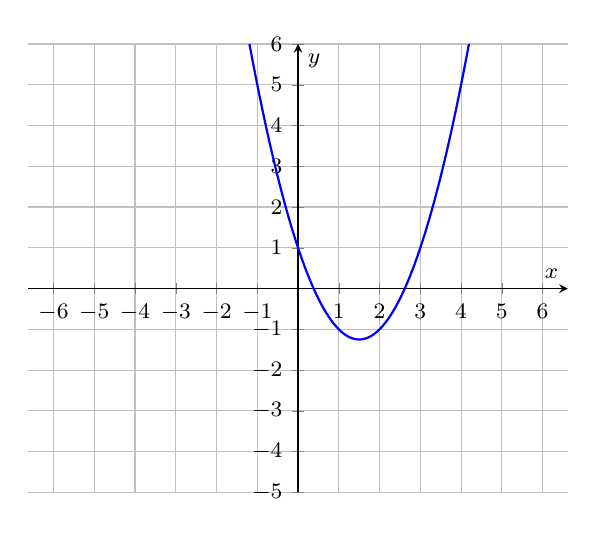
\begin{tikzpicture}
						\begin{axis}[
								axis equal,
								axis x line=middle,
								axis y line=middle,
								xlabel={$x$},
								ylabel={$y$},
								xtick distance=1,
								ytick distance=1,
								%			minor tick num = 2,
								xmin=-4, xmax=4,
								ymin=-5, ymax=6,
								grid=both,]
							\addplot[domain=-6:6,			samples=200,thick,color=blue,]{x^2-3*x+1};
						\end{axis}
					\end{tikzpicture}
				}
				\solonly{$y=x^2-3x+1$}
	
				\part
				\exonly{
					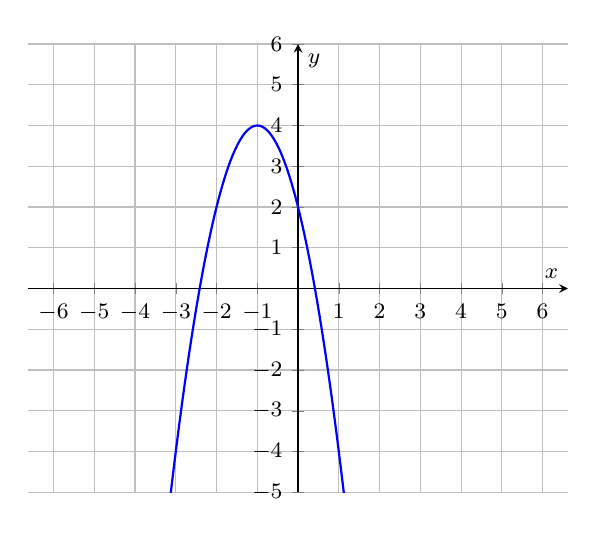
\begin{tikzpicture}
						\begin{axis}[
								axis equal,
								axis x line=middle,
								axis y line=middle,
								xlabel={$x$},
								ylabel={$y$},
								xtick distance=1,
								ytick distance=1,
								%			minor tick num = 2,
								xmin=-4, xmax=4,
								ymin=-5, ymax=6,
								grid=both,]
							\addplot[domain=-6:6,			samples=200,thick,color=blue,]{-2*x^2-4*x+2};
						\end{axis}
					\end{tikzpicture}
				}
				\solonly{$y=-2x^2-4x+2$}
	
				\part
				\exonly{
					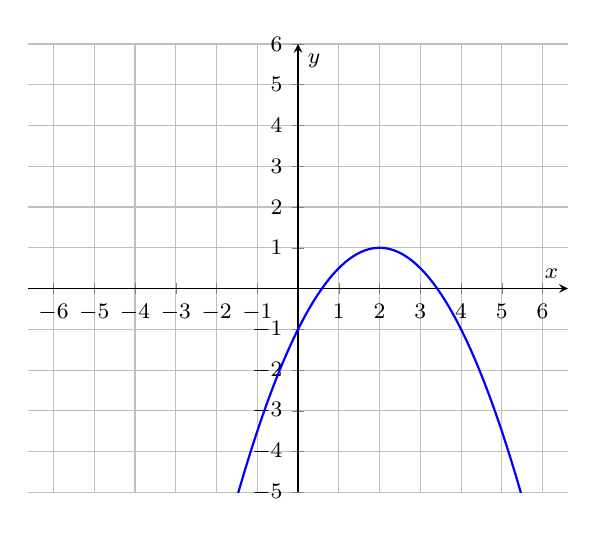
\begin{tikzpicture}
						\begin{axis}[
								axis equal,
								axis x line=middle,
								axis y line=middle,
								xlabel={$x$},
								ylabel={$y$},
								xtick distance=1,
								ytick distance=1,
								xmin=-4, xmax=4,
								ymin=-5, ymax=6,
								grid=both,]
							\addplot[domain=-6:6,			samples=200,thick,color=blue,]{-1/2*x^2+2*x-1};
						\end{axis}
					\end{tikzpicture}
				}
				\solonly{$y=-\frac{1}{2}x^2+2x-1$}
	
				\part
				\exonly{
					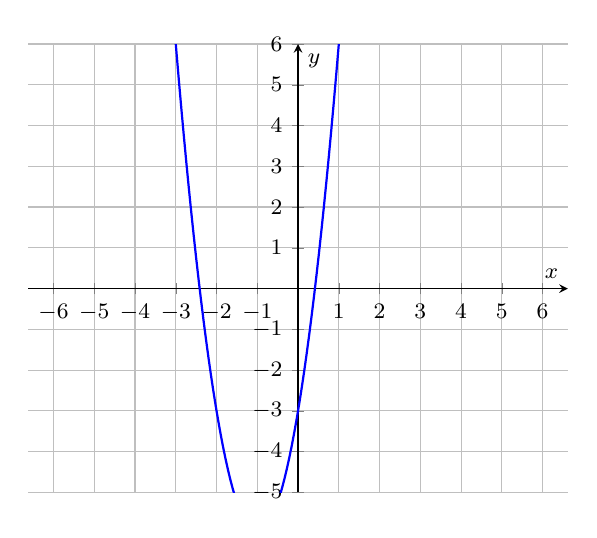
\begin{tikzpicture}
						\begin{axis}[
								axis equal,
								axis x line=middle,
								axis y line=middle,
								xlabel={$x$},
								ylabel={$y$},
								xtick distance=1,
								ytick distance=1,
								%			minor tick num = 2,
								xmin=-4, xmax=4,
								ymin=-5, ymax=6,
								grid=both,]
							\addplot[domain=-6:6,			samples=200,thick,color=blue,]{3*x^2+6*x-3};
						\end{axis}
					\end{tikzpicture}
				}
				\solonly{$y=3x^2+6x-3$}

				\part
				\exonly{
					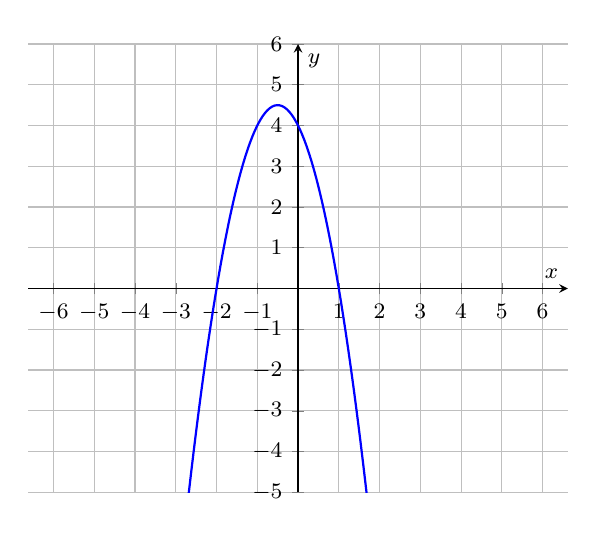
\begin{tikzpicture}
						\begin{axis}[
								axis equal,
								axis x line=middle,
								axis y line=middle,
								xlabel={$x$},
								ylabel={$y$},
								xtick distance=1,
								ytick distance=1,
								%			minor tick num = 2,
								xmin=-4, xmax=4,
								ymin=-5, ymax=6,
								grid=both,]
							\addplot[domain=-6:6,			samples=200,thick,color=blue,]{-2*(x-1)*(x+2)};
						\end{axis}
					\end{tikzpicture}
				}
				\solonly{$y=-2(x-1)(x+2)$}

				\part
				\exonly{
					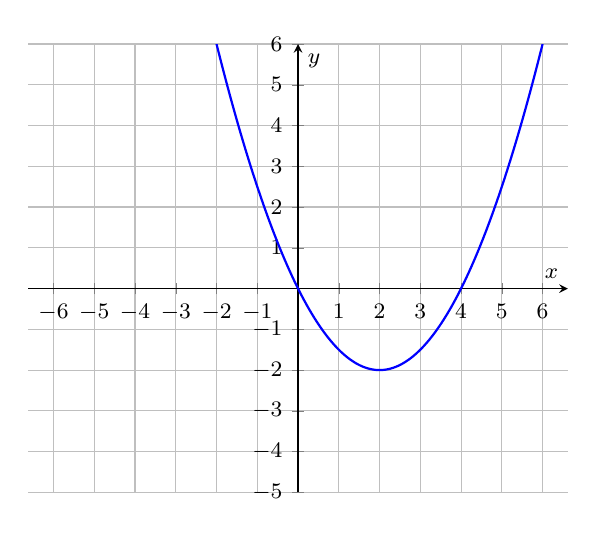
\begin{tikzpicture}
						\begin{axis}[
								axis equal,
								axis x line=middle,
								axis y line=middle,
								xlabel={$x$},
								ylabel={$y$},
								xtick distance=1,
								ytick distance=1,
								%			minor tick num = 2,
								xmin=-4, xmax=4,
								ymin=-5, ymax=6,
								grid=both,]
							\addplot[domain=-6:6,			samples=200,thick,color=blue,]{0.5*x*(x-4)};
						\end{axis}
					\end{tikzpicture}
				}
				\solonly{$y=\frac{1}{2}x(x-4)$}
			\end{parts}

			
		\end{multicols}
\end{qblock}


\end{questions}

\subsection{Applicazioni}
\begin{questions}

	
	\begin{qblock}
		\question
		\exonly{In un decreto  federale del 1889 è stato stipulato che: \textit{La bandiera della Confederazione consiste in una croce bianca verticale posta su di uno sfondo rosso le cui braccia, uguali tra loro, sono di un sesto più lunghe che larghe.}
	
			Per una festa si decide di dipingere la croce per terra utilizzando della pittura bianca. Quali saranno le dimensioni della croce se si vogliono usare \SI{204}{\square\metre} di pittura?}
	
		\solonly{Larghezza braccia \SI{6}{\metre}, lunghezza braccia \SI{7}{\metre}}
	\end{qblock}

	
	\begin{qblock}
		\question
		\exonly{Un giardino a forma rettangolare ha una lunghezza pari al doppio della sua larghezza. Un'aiuola larga \SI{3}{\metre} circonda questo giardino. Calcolare la larghezza del giardino sapendo che la superficie totale (giardino $+$ aiuola) è pari a \SI{360}{\square\metre}. }
	
		\solonly{Larghezza \SI{9}{\metre} }
	\end{qblock}

	
	\begin{qblock}
		\question
		\exonly{
			La'altezza $h(t)$ di un oggetto, lanciato verticalmente da un'altezza di \SI{1}{\metre} con una velocità di \SI{10}{m/s}, dopo $t$ secondi è data da:
	
			$$
				h(t)=-\dfrac{1}{2}gt^2+10t+1
			$$
	
			dove $g\approx \SI{9.81}{m/s^2}$ .
		}
		\begin{parts}
			\part
			\exonly{Dopo quanti secondi l'oggetto sarà ad un'altezza di \SI{3}{\metre}? (approssimare la risposta ai millisecondi)}
			\solonly{\SI{0.225}{\second} e \SI{1.814}{\second} }
			\part
			\exonly{Dopo quanti secondi l'oggetto sarà ad un'altezza di \SI{10}{\metre}? (approssimare la risposta ai millisecondi)}
			\solonly{Mai }
			\part
			\exonly{Qual'è l'altezza massima che può raggiungere? Dopo quanto tempo la raggiunge? }
			\solonly{Altezza massima \SI{6.097}{\metre} raggiunta dopo \SI{1.019}{\second} }
		\end{parts}
	\end{qblock}

	
	\begin{qblock}
		\question
		\exonly{
			Lo standard internazionale del formato carta, l'ISO 216, decreta che il formato A0 è un foglio di carta di \SI{1}{\square\metre} e che i formati successivi (A1, A2, \ldots) si ottengono semplicemente tagliando a metà la carta sul lato lungo. Per permettere di scalare da un formato all'altro senza compromettere l'aspetto si è deciso che il rapporto tra i due lati di un foglio deve essere costante.
		}
	
		\begin{parts}
			\part
			\exonly{Determinare, a partire dalla definizione, le dimensioni di un foglio di formato A0. }
			\solonly{$\SI{0.841}{\metre}\times\SI{1.189}{\metre}$ }
			\part
			\exonly{Determinare, a partire dalla definizione, le dimensioni di un foglio di formato A4. }
			\solonly{$\SI{21}{\centi\metre}\times\SI{29.7}{\centi\metre}$ }
		\end{parts}
	\end{qblock}




\begin{qblock}
		\question
		\exonly{
			La figura qui sotto mostra la sezione schematizzata di una casa.
	
			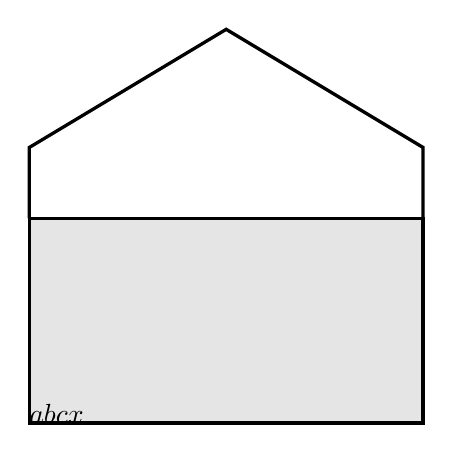
\begin{tikzpicture}
				\draw[very thick, fill=gray!20] (0,0) rectangle (5,2.6);
				\draw[very thick] (0,2.6) -- (0,3.5) -- (2.5,5) -- (5,3.5) -- (5,2.6);
				\dimline[extension start length=-0.3cm,extension end length=-0.3cm] {(0,-0.3)}{(5,-0.3)}{$a$};
				\dimline[extension end length=0.3cm,extension start length=0.3cm] {(-0.3,0)}{(-0.3,2.6)}{$b$};
				\dimline[extension end length=0.3cm,extension start length=0.3cm] {(-0.3,2.6)}{(-0.3,3.5)}{$c$};
				\dimline[extension end length=0,extension start length=0] {(2.5,2.6)}{(2.5,5)}{$x$};
			\end{tikzpicture}
	
		}
	
		\begin{parts}
			\part
			\exonly{Determinare l'altezza $x$ al centro del secondo piano affinché i due piani abbiano la stessa superficie di taglio}
			\solonly{$\es{2b-c}$}
	
			\part
			\exonly{
				Cosa potete constatare?
			}
			\solonly{La soluzione non dipende da $a$ ma solo da $b$ e $c$.}
	
		\end{parts}
\end{qblock}

	
	\begin{qblock}
		\question
		\exonly{Le pagine di un libro d'arte hanno forma rettangolare: larghezza pari a $a$ \si{\centi\metre} e lunghezza pari a
			$b$ \si{\centi\metre}.
	
			Ogni pagina è composta da una zona di testo e da un margine di larghezza costante $x$ \si{\centi\metre}.
	
			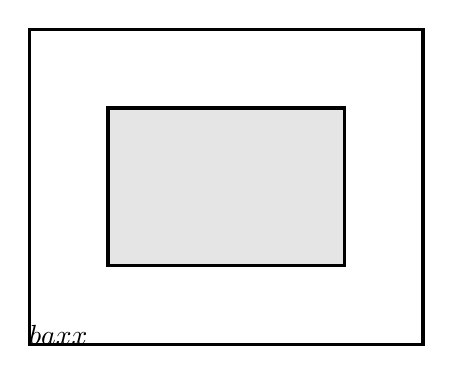
\begin{tikzpicture}
				\draw[very thick, fill=gray!20] (1,1) rectangle (4,3);
				\draw[very thick] (0,0) rectangle (5,4);
				\dimline[color=black,extension start length=-0.3cm, extension end length=-0.3cm] {(0,-0.3)}{(5,-0.3)}{$b$};
				\dimline[color=black,extension start length=0.3cm, extension end length=0.3cm] {(-0.3,0)}{(-0.3,4)}{$a$};
				\dimline[color=black,extension start length=0, extension end length=0] {(4,2)}{(5,2)}{$x$};
				\dimline[extension start length=0, extension end length=0] {(2.5,3)}{(2.5,4)}{$x$};
			\end{tikzpicture}
	
			Determinare la misura di tale margine affinché le due zone abbiano la stessa area.
		}
	
		\begin{parts}
			\part
			\exonly{Nel caso di un foglio A4 ($\SI{21}{\centi\metre}\times\SI{29.7}{\centi\metre}$.)
			}
			\solonly{\SI{3.58}{\centi\metre}}
	
			\part
	
			\exonly{Nel caso generale.}
			\solonly{$\dfrac{a+b-\sqrt{a^2+b^2}}{4}$}
	
		\end{parts}
	\end{qblock}

\end{questions}
\section{Geometria del piano}

\subsection{Angoli}

\begin{questions}
%%%%%%%%%%%%%%%%%%%%%%%%%%%%%%%%%%%%%%%%%%%%%%%%%%%%%%%%%%%%%%%%%
\question
\exonly{
Convertire in forma sessagesimale:
}

\begin{parts}
\part
\exonly{\ang{5,645}}  \solonly{\ang{5;38;42}}

\part
\exonly{\ang{15,37}}  \solonly{\ang{15;22;12}}

\part
\exonly{\ang{8,8}}  \solonly{\ang{8;48;}}
\end{parts}

%%%%%%%%%%%%%%%%%%%%%%%%%%%%%%%%%%%%%%%%%%%%%%%%%%%%%%%%%%%%%%%%%
\question
\exonly{

Convertire in gradi (forma decimale):
}

\begin{parts}
\part
\exonly{\ang{4;47;8} } \solonly{\ang{4.786}}

\part
\exonly{\ang{;895;}}  \solonly{\ang{14.92}}

\part
\exonly{\ang{12;38;24}}  \solonly{\ang{12.64}}
\end{parts}

%%%%%%%%%%%%%%%%%%%%%%%%%%%%%%%%%%%%%%%%%%%%%%%%%%%%%%%%%%%%%%%%%

\question
\exonly{

Convertire in gradi (forma decimale):
}

\begin{parts}
\part
\exonly{$\dfrac{\pi}{2}$} \solonly{\ang{90}}

\part
\exonly{$\dfrac{2}{3}\pi$}  \solonly{\ang{120}}

\part
\exonly{$\dfrac{5}{3}\pi$}  \solonly{\ang{300}}
\end{parts}

%%%%%%%%%%%%%%%%%%%%%%%%%%%%%%%%%%%%%%%%%%%%%%%%%%%%%%%%%%%%%%%%%

\question
\exonly{

Convertire in radianti (valore esatto):
}

\begin{parts}
\part
\exonly{\ang{30} } \solonly{$\dfrac{\pi}{6}$}

\part
\exonly{\ang{135}}  \solonly{$\dfrac{3}{4}\pi$}

\end{parts}

%%%%%%%%%%%%%%%%%%%%%%%%%%%%%%%%%%%%%%%%%%%%%%%%%%%%%%%%%%%%%%%%%

\question
\exonly{
	Calcolare l'angolo $\epsilon$ tra l'altezza $BH$ e la bisettrice $BI$ del vertice $B$.
}

\begin{parts}
\part
\exonly{
Nel caso particolare dove  $\angle ABC = 60^\circ$ e $\angle BCA= 40{}^\circ$.}
\solonly{$\epsilon=\ang{20}$}
\part
\exonly{In generale in funzione di  $\angle ABC = \alpha$ e $\angle BCA= \beta$ }
\solonly{$\epsilon=90 -\frac{\alpha}{2}-\beta$}
\end{parts}


\exonly{
\begin{tikzpicture}[line cap=round,line join=round,>=triangle 45,x=1.0cm,y=1.0cm,rotate=-30]
\draw (-1.0,3.0) node[left] {B}-- (3.0,3.0);
\draw (3.0,3.0) node[below right] {H}-- (3.0,0.0) ;
\draw (3.0,0.0) node[below] {A}-- (-1.0,3.0);
\draw (3.0,4.0)-- (-1.0,3.0);
\draw (3.0,4.0)-- (3.0,3.0);
\draw (3.0,6.0) node[right] {C}-- (3.0,4.0) node[below right] {I};
\draw (3.0,6.0)-- (-1.0,3.0) ;
\draw (2.8,3)--(2.8,3.2)--(3,3.2);
\draw (0,3) arc (0:14.04:1) node[right,midway,yshift=-0.1cm] {$\epsilon$} ;
\end{tikzpicture}
}

%%%%%%%%%%%%%%%%%%%%%%%%%%%%%%%%%%%%%%%%%%%%%%%%%%%%%%%%%%%%%%%%%%
%\question
%\exonly{
%\FR{
%Calculer les trois angles d`un triangle sachant que $2\cdot\alpha = \beta = \gamma$.
%}
%\DE{
%
%}}
%
%\solonly{$\alpha=\ang{36}$ \quad $\beta=\gamma=\ang{72}$
%}


%%%%%%%%%%%%%%%%%%%%%%%%%%%%%%%%%%%%%%%%%%%%%%%%%%%%%%%%%%%%%%%%%
\exnewpage
\question
\exonly{
Calcolare gli angoli $\gamma$ e $\delta$  in funzione di $\alpha$ e $\beta$:
%Calculer les angles $\gamma$ et $\delta$ en fonction de $\alpha$ et $\beta$ :
}

\begin{parts}
\part \exonly{
	se $ \alpha = 20^\circ$  e  $ \beta = 40^\circ$.}
\solonly{$\gamma=\ang{30}$ \quad  $\delta=\ang{30}$
}
\part \exonly{per $\alpha$ e $\beta$ qualunque.}
\solonly{$\gamma=\delta=90-\alpha -\beta$
}
\end{parts} 


%TODO : convert in TikZ
\includegraphics*[width=0.5\linewidth]{ch1-ex3}





%%%%%%%%%%%%%%%%%%%%%%%%%%%%%%%%%%%%%%%%%%%%%%%%%%%%%%%%%%%%%%%%%
%\question
%\exonly{
%\FR{
%Calculer les angles $\varphi_1$ à $\varphi_5$ si :
%$\alpha= 34^\circ$  et   $\delta = 60^\circ$.
%}
%\DE{
%
%}
%
%\includegraphics*[width=\linewidth]{ch1-ex4}
%}
%
%\solonly{
%$\varphi_1=\ang{124}$ \quad 
%$\varphi_2=\ang{112}$ \quad 
%$\varphi_3=\ang{128}$ \quad  \\
%$\varphi_4=\ang{142}$ \quad 
%$\varphi_5=\ang{68}$
%}



%%%%%%%%%%%%%%%%%%%%%%%%%%%%%%%%%%%%%%%%%%%%%%%%%%%%%%%%%%%%%%%%%

%\question
%\exonly{
%\FR{
%Calculer $\varphi$ à partir de $\alpha$:
%}
%\DE{
%
%}
%
%\includegraphics*[width=\linewidth]{ch1-ex5}
%}
%
%
%
%\begin{parts}
%\part
%\exonly{
%\FR{
%	pour $\alpha = \ang{36}$ 
%}
%\DE{
%	
%}}
%
%\solonly{$\varphi=\ang{117}$}
%
%
%\part
%\exonly{
%\FR{
%	pour un angle $\alpha$ quelconque
%}
%\DE{
%	
%}}
%
%\solonly{$\varphi=\ang{135} -\dfrac{\alpha}{2}$}
%
%
%\end{parts}




\end{questions}

%\exnewpage
%\subfile{../ch/5_2-Triangles_Semblables}
\subsection{Triangoli simili}
%\DE{\subsection{Änliches Dreiecks}}

\begin{questions}



%%%%%%%%%%%%%%%%%%%%%%%%%%%%%%%%%%%%%%%%%%%%%%%%%%%%%%%%%%%%%%%%%%%%%%%%
\question
\exonly{
Calcolare le misure mancanti $a$, $b$, $c$, $d$, $x$ e $y$ (in $\SI{}{\centi\meter}$) nei casi seguenti. Le rette $f$ e $g$ sono parallele.
}

%TODO : convert in TikZ
\exonly{\includegraphics*[width=0.5\linewidth]{ch2-ex3-1}}

\begin{parts}
\part 
\exonly{$a=\num{4.5}$ \quad $b=?$ \quad $c=3$  \quad  $d=2$ \\ $x=3$ \quad $y=?$}
\solonly{$b=3$ \quad $y=5$}

\part 
\exonly{$a=\num{6}$ \quad $b=?$ \quad $c=?$  \quad  $d=\num{1.6}$ \\ $x=5$ \quad $y=7$}
\solonly{$b=\num{2.4}$ \quad $c=4$}

\part 
\exonly{$a=?$ \quad $b=\num{4.2}$ \quad $c=\num{6.8}$  \quad  $d=\num{5.1}$ \\ $x=?$ \quad $y=\num{6.4}$}
\solonly{$a=\num{5.6}$ \quad $x=\num{3.66}$}

\part

\exonly{ $a=?$ \quad $b=\num{5.2}$ \quad $c=\num{2.8}$  \quad  $d=?$ \\ $x=\num{4.2}$ \quad $y=\num{8.1}$}
\solonly{$a=\num{5.6}$\quad $d=\num{2.6}$}

\part 
\exonly{$a=2$ \quad $b=\frac{7}{3}$ \quad $c=\frac{3}{2}$  \quad  $d=?$ \\ $x=\frac{6}{5}$ \quad $y=?$}
\solonly{$d=\frac{7}{4}=\num{1.75}$ \quad$y=\frac{13}{5}=\num{2.6}$}

\end{parts}


%%%%%%%%%%%%%%%%%%%%%%%%%%%%%%%%%%%%%%%%%%%%%%%%%%%%%%%%%%%%%%%%%%%%%%%%

%\question
%\exonly{
%\FR{Montrer que les triangles $ACB$ et $ADE$ sont semblables.
%
%Calculer $AD$ et $ED$ sans utiliser le théorème de Pythagore.
%
%$AB = 4$ ~ $BC = 3$ ~$AC = 5$ ~ $AE = 2$
%}
%}
%\exonly{\includegraphics*[width=0.6\linewidth]{ch2-ex1}}
%
%\solonly{$AD=\num{2.5}$ $ED=\num{1.5}$}

%%%%%%%%%%%%%%%%%%%%%%%%%%%%%%%%%%%%%%%%%%%%%%%%%%%%%%%%%%%%%%%%%%%%%%%%

\exnewpage
\question
\exonly{
A causa del lago non é possibile misurare la distanza $AC$.
Per poter calcolare questa distanza determiniamo i punti $B_1$ e $C_1$ tali per cui $B_1C_1$ sia parallela a $BC$.

Possiamo quindi misurare:   

$AB_{1}=\SI{15}{\meter}$ ~ $AC_{1}= \SI{9}{\meter}$ ~ $BB_{1}= \SI{133}{\meter}$.

Calcolare la distanza  $AC$.

}
\solonly{$AC=\SI{88.8}{\meter}$}

%TODO : convert in TikZ
\exonly{\includegraphics*[width=0.5\linewidth]{ch2-ex2}}


%%%%%%%%%%%%%%%%%%%%%%%%%%%%%%%%%%%%%%%%%%%%%%%%%%%%%%%%%%%%%%%%%%%%%%%%
%\question
%\exonly{
%\FR{
%Les diagonales d'un trapèze $ABCD$ se coupent en $O$.
%
%Calculer $OA$ sachant que les bases mesurent $AB = \SI{9}{\centi\meter}$ et $CD = \SI{6}{\centi\meter}$ et la diagonale $AC = \SI{10}{\centi\meter}$.
%}}
%
%\solonly{$OA=\SI{6}{\centi\meter}$}


%

%%%%%%%%%%%%%%%%%%%%%%%%%%%%%%%%%%%%%%%%%%%%%%%%%%%%%%%%%%%%%%%%%%%%%%%%
%\question
%\exonly{
%\FR{
%Quatre parallèles coupent deux droites sécantes $AC$ et $BD$.}}
%
%\begin{parts}
%\part
%\exonly{
%\FR{
%	Calculer $DF$ et $FH$ sachant que :
%	
%	$AC = 3$ ~$CE = 9$~ $EG = 6$ ~ $BD = 4$
%}} 
%\solonly{$DF=12$ \quad $FH=8$}
%
%\part
%\exonly{
%\FR{
%	Calculer $BD$ et $DF$ sachant que :
%	
%	$AC = 6$ ~$CE = 8$ ~$EG = 8$ ~ $BH = 33$
%}}
%
%\solonly{$BD=9$ \quad $DF=12$}
%\end{parts}
%
%
%\exonly{\includegraphics*[width=\linewidth]{ch2-ex5}}


%%%%%%%%%%%%%%%%%%%%%%%%%%%%%%%%%%%%%%%%%%%%%%%%%%%%%%%%%%%%%%%%%%%%%%%%
%\question
%\exonly{
%\FR{
%$f$, $g$ et $h$ sont trois droites parallèles.
%
%Calculer $AB$ et $CD$ lorsque $SB = \SI{7}{\centi\meter}$.
%}}
%
%
%\exonly{\includegraphics*[width=\linewidth]{ch2-ex6}}
%
%\solonly{$AB=\SI{5.6}{\centi\meter}$ \quad $CD=\SI{6}{\centi\meter}$k
%%%%%%%%%%%%%%%%%%%%%%%%%%%%%%%%%%%%%%%%%%%%%%%%%%%%%%%%%%%%%%%%%%%%%%%%%
%\exonly{\columnbreak}

%%%%%%%%%%%%%%%%%%%%%%%%%%%%%%%%%%%%%%%%%%%%%%%%%%%%%%%%%%%%%%%%%%%%%%%%

\question
\exonly{
Per determinare l'altezza di un palazzo un uomo si posiziona in modo da vedere la cima di un palo allineata alla cima del palazzo (altezza degli occhi  $\approx \SI{1.65}{\meter}$).

La distanza tra il palo (di altezza $\SI{3}{\meter}$) e il palazzo é di $\SI{33}{\meter}$ e quella tra il palo e la persone é di $\SI{7}{\meter}$


Calcolare l'altezza $h$ del palazzo.
}

\exonly{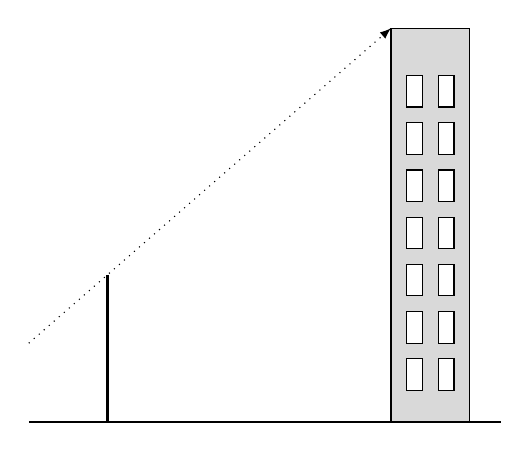
\begin{tikzpicture}
\human[0.5]{A}{0,0.5}
\draw[thick] (0,0) --(6,0);
\filldraw[fill=gray!30] (4.6,0) rectangle (5.6,5);
\draw[very thick] (1,0) -- (1,1.87);
%\draw[dotted,latex-latex] (0,1) -- node[above, midway] {\num{23.5}} (4.6,1);
\foreach \x in {0.2,0.8,1.4,2,2.6,3.2,3.8}
{
\filldraw[fill=white] (4.8, \x + 0.2) rectangle +(0.2,0.4) (5.2,0.2 + \x) rectangle +(0.2,0.4) ;
}
\draw[dotted,-latex] (0,1) -- (4.6,5);


\end{tikzpicture}}
%\exonly{\includegraphics*[width=\linewidth]{ch2-ex7}}
\solonly{$h=\SI{9.36}{\meter}$}

%%%%%%%%%%%%%%%%%%%%%%%%%%%%%%%%%%%%%%%%%%%%%%%%%%%%%%%%%%%%%%%%%%%%%%%%


%\question
%\exonly{
%\FR{
%Déterminer $x$, $y$ et $z$:
%}}
%\begin{parts}
%\part  
%\exonly{
%\FR{si}\DE{falls} $\! \!\!  a=\SI{6}{\centi\meter}$, $b=\SI{3}{\centi\meter}$, $c=\SI{5}{\centi\meter}$, $d=\SI{12}{\centi\meter}$, $e=\SI{8}{\centi\meter}$.}
%
%\solonly{$x=\num{13.33}$   $y=10$ $z=\num{7.2}$}
%
%\part \exonly{\FR{
%	en fonction de $a$, $b$, $c$, $d$ et $e$.
%	
%	C'est-à-dire: établir une formule permettant de calculer $x$ ($y$ et $z$) si on connaît les paramètres $a$, $b$, $c$, $d$ et $e$.}}
%
%\solonly{$x=\dfrac{ce}{b}$   $y=a\dfrac{e-b}{b}$ $z=\dfrac{bd}{e-b}$}
%\end{parts}
%
%\exonly{\includegraphics*[width=\linewidth]{ch2-ex8}}
%
%%%%%%%%%%%%%%%%%%%%%%%%%%%%%%%%%%%%%%%%%%%%%%%%%%%%%%%%%%%%%%%%%%%%%%%%%
%
%
%\question \exonly{\FR{
%$ABCD$ est un trapèze dont la base $c = CD$ est connue.
%
%$E$ est un point sur la base $AB$. Les longueurs $u$ et $v$ sont des paramètres connues.
%
%Déterminer $DF$ pour que les droites $AD$, $EF$ et $BC$ se coupent en un seul point:}}
%
%\begin{parts}
%\part 
%\exonly{
%\FR{si}\DE{falls} $u=\SI{5}{\centi\meter}$ , $v=\SI{3}{\centi\meter}$ \FR{et}\DE{und} $c=\SI{6}{\centi\meter}$
%}
%
%\solonly{$DF=\dfrac{30}{8}=\num{3.75}$}
%
%
%\part 
%\exonly{
%\FR{
%	en fonction de $u$, $v$ et $c$.}}
%
%\solonly{$DF=\dfrac{c \cdot u}{v + u}$}
%
%\end{parts}
%\exonly{\includegraphics*[width=\linewidth]{ch2-ex9}}
%
%%%%%%%%%%%%%%%%%%%%%%%%%%%%%%%%%%%%%%%%%%%%%%%%%%%%%%%%%%%%%%%%%%%%%%%%%
%\exonly{\columnbreak}
%
%%%%%%%%%%%%%%%%%%%%%%%%%%%%%%%%%%%%%%%%%%%%%%%%%%%%%%%%%%%%%%%%%%%%%%%%%
%
%\question  \exonly{\FR{
%$A$ et $B$ sont les centres de deux demi-cercles tangents de rayons $r$ et $R$.
%
%$AV$ et $BW$ sont deux rayons \textbf{parallèles} quelconques.
%
%Les droites $VW$ et $AB$ se coupent en $P$. (voir dessin) 
%}
%}
%\begin{parts}
%\part
%\exonly{\FR{ Calculer la distance $AP$ si $r = \SI{3}{\centi\meter}$ et $R = \SI{5}{\centi\meter}$}} \solonly{$AP=\SI{12}{\centi\meter}$}
%
%\part 
%\exonly{\FR{Déterminer une formule pour   $AP$ en fonction des paramètres  $r$ et $R$}} \solonly{$AP=\dfrac{r(R+r)}{R-r}$}
%
%
%\end{parts}
%
%\begin{tikzpicture}[scale=0.3]
%
%\exonly{
%\pgfmathsetmacro\r{3}
%\pgfmathsetmacro\R{5}
%\coordinate[label=below:$B$] (B) at (20,0);
%\coordinate (B1) at ($ (B) + (\R,0) $);
%\coordinate[label=below:$A$] (A) at (12,0);
%\coordinate (A1) at ($ (A) + (\r,0) $);
%\coordinate[label=below:$P$] (P) at (0,0);
%\draw (B1) arc (0:180:{\R});
%\draw (A1) arc (0:180:{\r});
%\draw (P) -- (B1);
%\coordinate[label=above:$W$] (W) at ($(B) + (120:{\R}) $);
%\coordinate[label=above:$V$] (V) at ($(A) + (120:{\r}) $);
%\draw (P) -- (W) --  node[midway, right] {$R$} (B);
%\draw (A) -- node[midway, right] {$r$} (V);
%}
%\end{tikzpicture}
%
%%\exonly{\includegraphics*[width=\linewidth]{ch2-ex10}}
%
%%
%
%
%%%%%%%%%%%%%%%%%%%%%%%%%%%%%%%%%%%%%%%%%%%%%%%%%%%%%%%%%%%%%%%%%%%%%%%%%
%
%\question \exonly{\FR{
%Soit $ABCD$ un quadrilatère avec  $AB=\SI{10}{\centi\metre}$, $BC=\SI{4}{\centi\metre}$,    $CD=\SI{12}{\centi\metre}$  et $AD=\SI{8}{\centi\metre}$.
%
%$S$ est le point d`intersection des diagonales.
%
%$P$ et $Q$ sont tels que $BC \parallel SP$ et $AB \parallel QS$.
%
%Sachant que $PC=\SI{5}{\centi\metre}$, déterminer $AQ$ et $QS$.
%}}
%
%\ifprintanswers   \else
%\begin{tikzpicture}
%\coordinate[label=below :$A$] (A) at (0,0); 
%\coordinate[label=below:$B$] (B) at (5,0);
%\coordinate[label=right:$C$] (C) at (6,2);
%\coordinate[label=above:$D$] (D) at (-1,4); 
%
%\draw[thick] (A) -- (B) -- (C) -- (D) -- cycle;
%\path[name path=DC] (D)--(C);
%\path[name path=DA] (D)--(A);
%\draw[name path=BD] (D) -- (B) ;
%\draw[name path=AC](A) -- (C);
%\path [name intersections={of=BD and AC,by=S}];
%\path (S) node [below] {$S$};
%\path[name path=SP] (S) -- +(1,2);
%\path [name intersections={of=DC and SP,by=P}];
%\draw (S) -- (P) node[above] {$P$};
%\path[name path=SA] (S) -- +(-5,0);
%\path [name intersections={of=DA and SA,by=Q}];
%\draw (S) -- (Q) node[left] {$Q$};
%
%\end{tikzpicture}  \fi
%\solonly{$AQ=\frac{10}{3}\approx \num{3.33}$ $QS=\frac{35}{6}\approx \num{5.83}$}
%
%

\todo[inline]{Trop d'ex?? }
\end{questions}
%
%%%\subfile{../ch/5_2-Triangles_Rectangles}
%
\exnewpage
\subsection{Triangolo rettangolo}
%\DE{\subsection{TODO}}



\begin{questions}
	
	%%%%%%%%%%%%%%%%%%%%%%%%%%%%%%%%%%%%%%%%%%%%%%%%%%%%%%%%%%%%%%%%%%%%%%%%
	
	\question
	\exonly{ %Borgeaud 2.7.1. a)
		
		Calcolare i lati e gli angoli mancanti del triangolo qui sotto:
	}
	
	\ifprintanswers   \else    
	
	%\hspace*{-3cm}
	\begin{tikzpicture}[scale=1.3]
		\tkzInit[xmin=-1,xmax=5,ymin=-5,ymax=0.5]
		\tkzClip
		\tkzDefPoint(0,0){A}
		\tkzDefShiftPoint[A](-90:4.1){B}
		\tkzDefShiftPoint[B](0:1.9){C}
		\tkzDrawPolygon(A,B,C) 
		\tkzLabelPoints[above](A)
		\tkzLabelPoints[below](B,C)
		\tkzLabelSegment[above right](C,A){$b$}
		\tkzLabelSegment[below](C,B){\SI{19}{\meter}}
		\tkzLabelSegment[left](A,B){\SI{41}{\meter}}
		\tkzDefLine[orthogonal=through B](C,A) \tkzGetPoint{h1}
		\tkzInterLL(C,A)(B,h1) \tkzGetPoint{H}
		\tkzDrawSegment(B,H)
		\tkzLabelSegment[above left](H,B){$h$}
		\tkzMarkRightAngle(B,H,A)
		\tkzMarkRightAngle(C,B,A)
		%\tkzLabelAngle[pos=0.7](A,C,B){$\gamma$}
		%\tkzMarkAngle[arc=l,size=.5 cm](A,C,B)
		%\tkzLabelAngle[pos=0.7](C,B,A){$\beta$}
		%\tkzMarkAngle[arc=l,size=.5 cm](C,B,A)
		%
		%\tkzLabelAngle[pos=0.7](C,A,B){$\alpha$}
		%\tkzMarkAngle[arc=l,size=.5 cm](B,A,C)
	\end{tikzpicture}
	\fi
	
	\solonly{$b=\SI{45.19}{\meter}$ \quad $\angle BCA=\ang{65.14}$  \\ $\angle CAB= \ang{24.86}$  \quad $h=\SI{17.24}{\meter}$
	}
	
	%%%%%%%%%%%%%%%%%%%%%%%%%%%%%%%%%%%%%%%%%%%%%%%%%%%%%%%%%%%%%%%%
	
	\question
	\exonly{%Borgeaud 2.7.1. b)
		Calcolare i lati e gli angoli mancanti del triangolo qui sotto:}
	
	\ifprintanswers   \else  
	\begin{tikzpicture}[scale=1.5]
		\tkzDefPoint(0,0){C}
		\tkzDefShiftPoint[C](-90:4.1){A}
		\tkzDefShiftPoint[C](0:1.9){B}
		\tkzDrawPolygon(A,B,C) 
		\tkzLabelPoints[above](C,B)
		\tkzLabelPoints[below](A)
		\tkzLabelSegment[left](C,A){$b$}
		\tkzLabelSegment[above](C,B){$a$}
		\tkzLabelSegment[right](A,B){\SI{105}{\meter}}
		\tkzLabelAngle[pos=1](B,A,C){$\ang{38}$}
		\tkzMarkAngle[arc=l,size=.5 cm](B,A,C)
		\tkzMarkRightAngle(B,C,A)
	\end{tikzpicture}
	\fi
	
	\solonly{$b=\SI{82.74}{\meter}$  $\angle CBA=\ang{52}$  \\ $a=\SI{64.64}{\meter}$
	}
	
	%\exnewpage
	%%%%%%%%%%%%%%%%%%%%%%%%%%%%%%%%%%%%%%%%%%%%%%%%%%%%%%%%%%%%%%%%
	\question
	\exonly{ %Borgeaud 2.7.1. c)
		Calcolare i lati e gli angoli mancanti del triangolo qui sotto:
	}
	
	\ifprintanswers   \else 
	
	\begin{tikzpicture}[scale=1.5]
		\tkzDefPoint(0,0){A}
		\tkzDefShiftPoint[A](-90:3){B}
		\tkzDefShiftPoint[B](0:4){C}
		\tkzDrawPolygon(A,B,C) 
		\tkzLabelPoints[below](C,B)
		\tkzLabelPoints[above](A)
		\tkzLabelSegment[above right](C,A){$b$}
		\tkzLabelSegment[below](C,B){\SI{30}{\meter}}
		\tkzLabelSegment[left](A,B){\SI{25}{\meter}}
		\tkzMarkRightAngle(C,B,A)
	\end{tikzpicture}
	\fi
	
	\solonly{$b=\SI{39.05}{\meter}$  $\angle BCA=\ang{39.81}$  \\ $\angle BAC=\ang{50.19}$
	}
	%%%%%%%%%%%%%%%%%%%%%%%%%%%%%%%%%%%%%%%%%%%%%%%%%%%%%%%%%%%%%%%%
	
	\question
	\exonly{%Borgeaud 2.7.1. d)
		Calcolare i lati e gli angoli mancanti del triangolo qui sotto:
	}
	
	\ifprintanswers   \else 
	\begin{tikzpicture}[scale=0.8]
		\tkzDefPoint(0,0){A}
		\tkzDefShiftPoint[A](-90:3){B}
		\tkzDefShiftPoint[B](0:8){C}
		\tkzDrawPolygon(A,B,C) 
		\tkzLabelPoints[below](C,B)
		\tkzLabelPoints[above](A)
		\tkzLabelSegment[above right](C,A){\SI{50}{\meter}}
		\tkzLabelSegment[below](C,B){$a$}
		\tkzLabelSegment[left](A,B){$c$}
		\tkzMarkRightAngle(C,B,A)
		\tkzLabelAngle[pos=1.1](B,A,C){\footnotesize $1,2^{rad}$}
		\tkzMarkAngle[arc=l,size=.5 cm](B,A,C)
	\end{tikzpicture}
	\fi
	
	\solonly{$a=\SI{46.6}{\meter}$  $\angle BCA=\ang{21.25}$  \\ $c=\SI{18.12}{\meter}$
	}
	%%%%%%%%%%%%%%%%%%%%%%%%%%%%%%%%%%%%%%%%%%%%%%%%%%%%%%%%%%%%%%%%
	
	\question
	\exonly{%Borgeaud 2.7.4
		
		
		Qual'é l'altezza di una torre che proietta al suolo un ombra di \SI{96}{\metre} quando il sole forma un angolo \ang{52.5}  di con l'orizzonte?
		
	}
	\solonly{$\SI{125.11}{\meter}$}
	
	%%%%%%%%%%%%%%%%%%%%%%%%%%%%%%%%%%%%%%%%%%%%%%%%%%%%%%%%%%%%%%%%
	
	\question
	\exonly{%Borgeaud 2.7.5
		
		Determinare l'angolo formato dai raggi di sole e l'orizzonte se  se l'ombra di un palo vale  $\num{1.5}$ la sua altezza?
		
		%Quale angolo tra i raggi di soloe e l'orizzonte se l'ombra di un palo vale  $\num{1.5}$ la sua altezza?
	}
	
	\solonly{\ang{33.69}}
	
	%%%%%%%%%%%%%%%%%%%%%%%%%%%%%%%%%%%%%%%%%%%%%%%%%%%%%%%%%%%%%%%%
	
	%\question
	%\exonly{%Borgeaud 2.7.6
	%\FR{
	%Un mur de \SI{7.5}{\meter} de haut est à $5$ m d'une maison. Quelle serait la longueur la plus courte d'une échelle qui, partant du sol, puisse juste s'appuyer sur le haut du mur et atteindre une fenêtre située à \SI{10.2}{\meter} du sol?
	%}
	%\DE{}
	%}
	%
	%\solonly{\SI{21.47}{\meter}}
	%%%%%%%%%%%%%%%%%%%%%%%%%%%%%%%%%%%%%%%%%%%%%%%%%%%%%%%%%%%%%%%%%
	
	
	
	
\end{questions}
\exnewpage
\subsection{Angolo al centro}
%\DE{\subsection{TODO}}

\begin{questions}

\question
\exonly{Calcolare $\alpha$, $\beta$, $\gamma$ e $\delta$.}

%TODO : convert in TikZ
\exonly{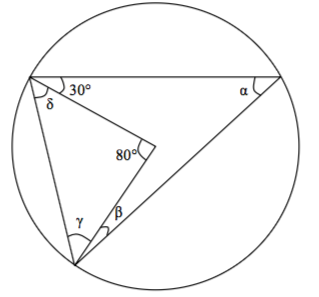
\includegraphics[width=0.5\linewidth]{aac-1}}

\solonly{$\alpha=40^{\circ}$, $\gamma=\delta=50^{\circ}$, $\beta=10^{\circ}$}

\question
\exonly{Calcolare $\alpha$, $\beta$, $\gamma$ e $\delta$.}

\exonly{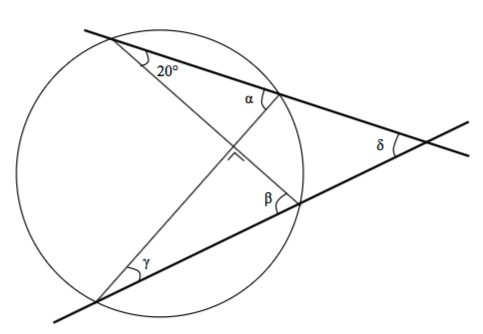
\includegraphics[width=0.6\linewidth]{aac-2}}

\solonly{$\gamma=20^{\circ}$, $\alpha=\beta=70^{\circ}$, $\delta=50^{\circ}$}

%\question
%\exonlyFR{Calculer les angles $\alpha$ et $\beta$ en sachant que $\gamma=80^{\circ}$ et $\delta=110^{\circ}$.}
%
%\exonly{\includegraphics[scale=0.8]{aac-3}}
%\solonly{$\alpha=100^{\circ}$, $\beta=70^{\circ}$}
%
%\question
%\exonlyFR{Un hélicoptère s'élève à la verticale d'un point A. 
%
%Sur le sol se trouvent trois points $A$, $B$ et $C$ alignés (dans cet ordre) tels que $AB = \SI{400}{\meter}$ et $BC = \SI{1}{\kilo\meter}$.
%
%L'hélicoptère voit les points $B$ et $C$ sous un angle de $30^\circ$.
%}
%
%\begin{parts}
%\part
%\exonlyFR{Faire un croquis de la situation.}
%
%\part
%\exonly{Dessiner l'ensemble des points $H'$ tels que $\angle{BH'C}=30^{\circ}$}
%
%\part
%\exonly{Calculer l'altitude de l'hélicoptère}
%\solonly{$h_1=\SI{430}{\meter}$, $h_2=\SI{1300}{\meter}$}
%\end{parts}




\end{questions}


%%\subfile{../ch/5_2-Droites-rem-cercles}
%\subsection{Droites remarquables, cercle inscrit et circonscrit}
%%\DE{\subsection{TODO}}
%
%\begin{questions}
%\begin{multicols}{2}
%
%\question
%\exonlyFR{
%Soit $ABC$ un triangle avec $a = 8$, $b = 9$ et $c = 14$. Calculer les rayons des cercles inscrit et circonscrit au triangle, son aire, la longueur des trois hauteurs et les trois angles du triangle.}
%\solonly{
%$r\approx\num{2.17}$ , $R\approx \num{7.48}$, $A\approx \num{33.67}$
%
%$h_A\approx \num{8.42}$, $h_B\approx \num{7.48}$, $h_C \approx \num{4.81}$
%}
%
%
%
%\question
%\exonlyFR{
%Soit $ABC$ un triangle rectangle en $C$ avec $a = 8$ et $b = 15$.  Calculer les rayons des cercles inscrit et circonscrit au triangle, son aire, la longueur des trois hauteurs et les trois angles du triangle.}
%\solonly{
%$r=3$ , $R=8.5$, $A=60$
%
%$h_A=b=15$, $h_B=a=8$, $h_C \approx \num{7.06}$
%}
%
%
%
%\question
%\exonly{
%Calculer les rayons des cercles inscrit et circonscrit à un triangle équilatéral de côté $a$.
%}
%\solonly{
%$r=\dfrac{\sqrt{3}}{6}a$ , $R=\dfrac{3 \sqrt{3}}{3}$, $A=\dfrac{\sqrt{3}}{4}a^2$
%}
%
%
%\question
%\exonly{
%Calculer les rayons des deux cercles inscrits dans un triangle isocèle de hauteur $h = 12$ cm et de base 10 cm.
%
%Le petit cercle est inscrit entre les deux côtés du triangle et le cercle inscrit au triangle.
%}
%\exonly{
%\includegraphics*[scale=1.3]{ch6-ex4}
%}
%
%\solonly{$r\approx \num{1.48}$, $R\approx 3,\!\overline{3}$}
%
%\todo[inline]{Ex sur les droites remarquables??}
%
%\end{multicols}
%\end{questions}
%
%\subsection{Triangolo rettangolo}
%\DE{\subsection{TODO}}


%\subsection{Triangolo rettangolo}
%\begin{questions}
%
%%%%%%%%%%%%%%%%%%%%%%%%%%%%%%%%%%%%%%%%%%%%%%%%%%%%%%%%%%%%%%%%%%%%%%%%%
%
%\question
%\exonly{ %Borgeaud 2.7.1. a)
%
%Calcolare i lati e gli angoli mancanti del triangolo qui sotto:
%}
%
%\ifprintanswers   \else     
%\begin{tikzpicture}[scale=1.3]
%\tkzInit[xmin=-1,xmax=5,ymin=-5,ymax=0.5]
%\tkzClip
%\tkzDefPoint(0,0){A}
%\tkzDefShiftPoint[A](-90:4.1){B}
%\tkzDefShiftPoint[B](0:1.9){C}
%\tkzDrawPolygon(A,B,C) 
%\tkzLabelPoints[above](A)
%\tkzLabelPoints[below](B,C)
%\tkzLabelSegment[above right](C,A){$b$}
%\tkzLabelSegment[below](C,B){\SI{19}{\meter}}
%\tkzLabelSegment[left](A,B){\SI{41}{\meter}}
%\tkzDefLine[orthogonal=through B](C,A) \tkzGetPoint{h1}
%\tkzInterLL(C,A)(B,h1) \tkzGetPoint{H}
%\tkzDrawSegment(B,H)
%\tkzLabelSegment[above left](H,B){$h$}
%\tkzMarkRightAngle(B,H,A)
%\tkzMarkRightAngle(C,B,A)
%%\tkzLabelAngle[pos=0.7](A,C,B){$\gamma$}
%%\tkzMarkAngle[arc=l,size=.5 cm](A,C,B)
%%\tkzLabelAngle[pos=0.7](C,B,A){$\beta$}
%%\tkzMarkAngle[arc=l,size=.5 cm](C,B,A)
%%
%%\tkzLabelAngle[pos=0.7](C,A,B){$\alpha$}
%%\tkzMarkAngle[arc=l,size=.5 cm](B,A,C)
%\end{tikzpicture}
%\fi
%
%\solonly{$b=\SI{45.19}{\meter}$ \quad $\angle BCA=\ang{65.14}$  \\ $\angle CAB= \ang{24.86}$  \quad $h=\SI{17.24}{\meter}$
%}
%
%%%%%%%%%%%%%%%%%%%%%%%%%%%%%%%%%%%%%%%%%%%%%%%%%%%%%%%%%%%%%%%%%
%
%\question
%\exonly{%Borgeaud 2.7.1. b)
%Calcolare i lati e gli angoli mancanti del triangolo qui sotto:
%
%\ifprintanswers   \else     
%\begin{tikzpicture}[scale=1.5]
%\tkzDefPoint(0,0){C}
%\tkzDefShiftPoint[C](-90:4.1){A}
%\tkzDefShiftPoint[C](0:1.9){B}
%\tkzDrawPolygon(A,B,C) 
%\tkzLabelPoints[above](C,B)
%\tkzLabelPoints[below](A)
%\tkzLabelSegment[left](C,A){$b$}
%\tkzLabelSegment[above](C,B){$a$}
%\tkzLabelSegment[right](A,B){\SI{105}{\meter}}
%\tkzLabelAngle[pos=1](B,A,C){$\ang{38}$}
%\tkzMarkAngle[arc=l,size=.5 cm](B,A,C)
%\tkzMarkRightAngle(B,C,A)
%\end{tikzpicture}
%\fi
%
%\solonly{$b=\SI{82.74}{\meter}$  $\angle CBA=\ang{52}$  \\ $a=\SI{64.64}{\meter}$
%}
%
%\exnewpage
%%%%%%%%%%%%%%%%%%%%%%%%%%%%%%%%%%%%%%%%%%%%%%%%%%%%%%%%%%%%%%%%%
%\question
%\exonly{ %Borgeaud 2.7.1. c)
%Calcolare i lati e gli angoli mancanti del triangolo qui sotto:
%
%
%\begin{tikzpicture}[scale=1.5]
%\tkzDefPoint(0,0){A}
%\tkzDefShiftPoint[A](-90:3){B}
%\tkzDefShiftPoint[B](0:4){C}
%\tkzDrawPolygon(A,B,C) 
%\tkzLabelPoints[below](C,B)
%\tkzLabelPoints[above](A)
%\tkzLabelSegment[above right](C,A){$b$}
%\tkzLabelSegment[below](C,B){\SI{30}{\meter}}
%\tkzLabelSegment[left](A,B){\SI{25}{\meter}}
%\tkzMarkRightAngle(C,B,A)
%\end{tikzpicture}
%}
%
%\solonly{$b=\SI{39.05}{\meter}$  $\angle BCA=\ang{39.81}$  \\ $\angle BAC=\ang{50.19}$
%}
%%%%%%%%%%%%%%%%%%%%%%%%%%%%%%%%%%%%%%%%%%%%%%%%%%%%%%%%%%%%%%%%%
%
%\question
%\exonly{%Borgeaud 2.7.1. d)
%Calcolare i lati e gli angoli mancanti del triangolo qui sotto:
%
%\begin{tikzpicture}[scale=0.8]
%\tkzDefPoint(0,0){A}
%\tkzDefShiftPoint[A](-90:3){B}
%\tkzDefShiftPoint[B](0:8){C}
%\tkzDrawPolygon(A,B,C) 
%\tkzLabelPoints[below](C,B)
%\tkzLabelPoints[above](A)
%\tkzLabelSegment[above right](C,A){\SI{50}{\meter}}
%\tkzLabelSegment[below](C,B){$a$}
%\tkzLabelSegment[left](A,B){$c$}
%\tkzMarkRightAngle(C,B,A)
%\tkzLabelAngle[pos=1.1](B,A,C){\footnotesize $1,2^{rad}$}
%\tkzMarkAngle[arc=l,size=.5 cm](B,A,C)
%\end{tikzpicture}
%
%}
%
%\solonly{$a=\SI{46.6}{\meter}$  $\angle BCA=\ang{21.25}$  \\ $c=\SI{18.12}{\meter}$
%}
%%%%%%%%%%%%%%%%%%%%%%%%%%%%%%%%%%%%%%%%%%%%%%%%%%%%%%%%%%%%%%%%%
%
%\question
%\exonly{%Borgeaud 2.7.4
%
%
%Qual'é l'altezza di una torre che proietta al suolo un ombra di \SI{96}{\metre} quando il sole forma un angolo \ang{52.5}  di con l'orizzonte?
%
%}
%\solonly{$\SI{125.11}{\meter}$}
%
%%%%%%%%%%%%%%%%%%%%%%%%%%%%%%%%%%%%%%%%%%%%%%%%%%%%%%%%%%%%%%%%%
%
%\question
%\exonly{%Borgeaud 2.7.5
%
%Determinare l'angolo formato dai raggi di sole e l'orizzonte se  se l'ombra di un palo vale  $\num{1.5}$ la sua altezza?
%
%%Quale angolo tra i raggi di soloe e l'orizzonte se l'ombra di un palo vale  $\num{1.5}$ la sua altezza?
%}
%
%\solonly{\ang{33.69}}
%
%%%%%%%%%%%%%%%%%%%%%%%%%%%%%%%%%%%%%%%%%%%%%%%%%%%%%%%%%%%%%%%%%
%
%%\question
%%\exonly{%Borgeaud 2.7.6
%%\FR{
%%Un mur de \SI{7.5}{\meter} de haut est à $5$ m d'une maison. Quelle serait la longueur la plus courte d'une échelle qui, partant du sol, puisse juste s'appuyer sur le haut du mur et atteindre une fenêtre située à \SI{10.2}{\meter} du sol?
%%}
%%\DE{}
%%}
%%
%%\solonly{\SI{21.47}{\meter}}
%%%%%%%%%%%%%%%%%%%%%%%%%%%%%%%%%%%%%%%%%%%%%%%%%%%%%%%%%%%%%%%%%%
%
%
%
%
%\end{questions}


\exnewpage
\subsection{Triangoli qualunque}

\begin{questions}

%%%%%%%%%%%%%%%%%%%%%%%%%%%%%%%%%%%%%%%%%%%%%%%%%%%%%%%%%%%%%%%%%%%%%%%%


\question
\exonly{
	Calcolare l'area dei triangoli qui sotto nelle situazioni date:
%	Calculer l'aire du triangle ci-dessous pour le situations suivantes:
}

\ifprintanswers   \else     
%\begin{adjustbox}{width=\linewidth}
\begin{tikzpicture}%[every node/.style={opacity=1, black, above left}] 
\path (0,0) coordinate (A)  node[left] {$A$};
\path (5,0) coordinate (B) node[right] {$B$};
\path (3,2) coordinate (C) node[above] {$C$};
\path (A) -- (B) node[midway,below] {$c$};
\path (B) -- (C) node[midway,above] {$a$};
\path (C) -- (A) node[midway,above] {$b$};
%\path ($(A)!0.5!(B)$) node [below] {$c$} ;
%\node at ($(A)!0.5!(B)$) [below] {$c$}  ;
%\node at ($(A)!0.5!(C)$) [above ] {$b$}  ;
%\node at ($(C)!0.5!(B)$) [above] {$a$}  ;
\draw (A)--(B)--(C) --cycle;
\path 
pic[pic text=$\alpha$,draw,angle eccentricity=1.5] {angle=B--A--C}
pic[pic text=$\beta$,draw,angle eccentricity=1.5] {angle=C--B--A}
pic[pic text=$\gamma$,draw,angle eccentricity=1.5] {angle=A--C--B}
;

\end{tikzpicture}
\fi

\begin{parts}
\part \exonly{$\alpha=\ang{40}$, $b=\SI{38}{\meter}$, $c=\SI{25}{\meter}$}
\solonly{\SI{305.32}{\square\meter}}

\part
\exonly{$\alpha =\ang{31}$, $\gamma=\ang{40}$, $a=\SI{53}{\meter}$}
\solonly{\SI{1657.47}{\square\meter}}

\end{parts}


%%%%%%%%%%%%%%%%%%%%%%%%%

\question
\exonly{
	Calcolare $\alpha$, $\beta$ e $\gamma$.
	}


\ifprintanswers   \else 
%\begin{tikzpicture}[scale=0.7]
%\tkzDefPoint(0,0){B}
%\tkzDefShiftPoint[B](35:5){C}
%\tkzDefShiftPoint[B](100:6){A}
%\tkzDrawPolygon(A,B,C) 
%\tkzLabelPoints[below](C,B)
%\tkzLabelPoints[above](A)
%\tkzLabelSegment[below right](C,B){$\SI{5}{\meter}$}
%\tkzLabelSegment[left](A,B){$\SI{7}{\meter}$}
%\tkzLabelSegment[above right](A,C){$\SI{6}{\meter}$}
%\tkzLabelAngle[pos=1.2](B,A,C){$\alpha$}
%\tkzMarkAngle[arc=l,size=.8 cm](B,A,C)
%\tkzLabelAngle[pos=-1.2](B,C,A){$\gamma$}
%\tkzMarkAngle[arc=l,size=.8 cm](A,C,B)
%\tkzLabelAngle[pos=0.8](A,B,C){$\beta$}
%\tkzMarkAngle[arc=l,size=.5 cm](C,B,A)
%\end{tikzpicture}


\begin{tikzpicture}[scale=0.7]
\coordinate[label=below :$B$]  (B) at (0,0);
\coordinate[label= right:$C$]  (C) at (35:5);
\coordinate[label=above:$A$]  (A) at (100:6);
\draw (A) -- node[midway, left] {$\SI{7}{\meter}$} (B) --node[midway, below right] {$\SI{5}{\meter}$} (C) --node[midway, above right] {$\SI{6}{\meter}$} cycle;
\path 
pic[pic text=$\alpha$,draw,angle eccentricity=1.5] {angle=B--A--C}
pic[pic text=$\beta$,draw,angle eccentricity=1.5] {angle=C--B--A}
pic[pic text=$\gamma$,draw,angle eccentricity=1.5] {angle=A--C--B};
\end{tikzpicture}
\fi

\solonly{$\alpha \approx \num{44.42}^{\circ}$, $\beta \approx \num{57.12}^{\circ}$, $\gamma \approx \num{78.46}^{\circ}$}

%%%%%%%%%%%%%%%%%%%%%%%%%%%%%%%%%%%%%%%%%%%%%%%%%%%%%%%%%%%%%%%
%
%\question
%\exonly{
%\FR{
%Un ballon $S$ et deux observateurs $A$ et $B$ se trouvent dans le même plan vertical.
%On a mesuré $AB=\SI{400}{\meter}$, $\angle BAS = \ang{55}$ et $\angle ABS = \ang{45}$.
%
%Calculer la hauteur $h$ du ballon.
%}
%\DE{
%
%}}
%
%\solonly{
%$h=\SI{235.27}{\meter}$
%}
%
%


%%%%%%%%%%%%%%%%%%%%%%%%%%%%%%%%%%%%%%%%%%%%%%%%%%%%%%%%%%%%%%%

\question
\exonly{
Calcolare $c$, $\beta$ e $\gamma$.}

\ifprintanswers   \else  
%\begin{tikzpicture}[scale=0.7]
%\tkzDefPoint(0,0){B}
%\tkzDefShiftPoint[B](0:5){C}
%\tkzDefShiftPoint[B](76:6){A}
%\tkzDrawPolygon(A,B,C) 
%\tkzLabelPoints[below](C,B)
%\tkzLabelPoints[above](A)
%\tkzLabelSegment[below](C,B){$\SI{5}{\meter}$}
%\tkzLabelSegment[left](A,B){$c$}
%\tkzLabelSegment[above right](A,C){$\SI{7}{\meter}$}
%\tkzLabelAngle[pos=1.2](B,A,C){$35^{\circ}$}
%\tkzMarkAngle[arc=l,size=.8 cm](B,A,C)
%\tkzLabelAngle[pos=1.2](B,C,A){$\gamma$}
%\tkzMarkAngle[arc=l,size=.8 cm](A,C,B)
%\tkzLabelAngle[pos=0.8](A,B,C){$\beta$}
%\tkzMarkAngle[arc=l,size=.5 cm](C,B,A)
%\end{tikzpicture}

\begin{tikzpicture}[scale=0.7]
\coordinate[label=below :$B$]  (B) at (0,0);
\coordinate[label= right:$C$]  (C) at (0:5);
\coordinate[label=above:$A$]  (A) at (76:6);
\draw (A) -- node[midway, left] {$c$} (B) --node[midway, below ] {$\SI{5}{\meter}$} (C) --node[midway, above right] {$\SI{7}{\meter}$} cycle;
\path 
pic[pic text=$35\degree$,draw,angle eccentricity=1.5] {angle=B--A--C}
pic[pic text=$\beta$,draw,angle eccentricity=1.5] {angle=C--B--A}
pic[pic text=$\gamma$,draw,angle eccentricity=1.5] {angle=A--C--B};
\end{tikzpicture}
\fi

\solonly{$\beta_1 \approx \num{53.42}^{\circ}$, $\gamma_1 \approx \num{91.58}^{\circ}$, $c_1\approx \SI{8.71}{\meter}$}

\solonly{$\beta_2 \approx \num{126.58}^{\circ}$, $\gamma_2 \approx \num{18.42}^{\circ}$, $c_2\approx \SI{2.75}{\meter}$}

%%%%%%%%%%%%%%%%%%%%%%%%%%%%%%%%%%%%%%%%%%%%%%%%%%%%%%%%%%%%%%%%%%%%%%%%%
\exnewpage
\question
\exonly{
Calcolare $c$, $\alpha$, $\beta$ e $\gamma$ se l'area del triangolo é di $\SI{12}{\square\meter}$.
}

\exonly{
%\begin{tikzpicture}[scale=0.7]
%\tkzDefPoint(0,0){B}
%\tkzDefShiftPoint[B](0:3){C}
%\tkzDefShiftPoint[B](64:5){A}
%\tkzDrawPolygon(A,B,C) 
%\tkzLabelPoints[below](C,B)
%\tkzLabelPoints[above](A)
%\tkzLabelSegment[below](C,B){$\SI{6}{\meter}$} %CB
%\tkzLabelSegment[left](A,B){$c$}  % AB
%\tkzLabelSegment[above right](A,C){$\SI{5}{\meter}$} %AC
%\tkzLabelAngle[pos=1.2](B,A,C){$\alpha$} %alpha
%\tkzMarkAngle[arc=l,size=.8 cm](B,A,C)
%\tkzLabelAngle[pos=1.2](B,C,A){$\gamma$} %gamma
%\tkzMarkAngle[arc=l,size=.8 cm](A,C,B)
%\tkzLabelAngle[pos=0.8](A,B,C){$\beta$} %beta
%\tkzMarkAngle[arc=l,size=.5 cm](C,B,A)
%\end{tikzpicture}
\begin{tikzpicture}[scale=0.8]
\coordinate[label=below :$B$]  (B) at (0,0);
\coordinate[label= right:$C$]  (C) at (0:3);
\coordinate[label=above:$A$]  (A) at (64:5);
\draw (A) -- node[midway, left] {$c$} (B) --node[midway, below ] {$\SI{6}{\meter}$} (C) --node[midway, above right] {$\SI{5}{\meter}$} cycle;
\path 
pic[pic text=$\alpha$,draw,angle eccentricity=1.5] {angle=B--A--C}
pic[pic text=$\beta$,draw,angle eccentricity=1.5] {angle=C--B--A}
pic[pic text=$\gamma$,draw,angle eccentricity=1.5] {angle=A--C--B};
\end{tikzpicture}
}

\solonly{$\alpha_1 \approx \ang{73.74}$, $\beta_1 \approx \ang{53.13}$ \\$\gamma_1 \approx \ang{53.13}$, $c_1\approx \SI{5}{\meter}$}

\solonly{$\alpha_2 \approx \ang{29.16}$, $\beta_2 \approx \ang{23.97}$ \\ $\gamma_2 \approx \ang{126.87}$, $c_2\approx \SI{9.85}{\meter}$}


\question
\exonly{
Per stimare l'altezza di una montagna per triangolazione un osservatore misura l'angolo di elevazione $\alpha=\ang{25}$ (angolo tra l'orizzontale e la cima della montagna). In seguito, spostandosi sullo sullo stesso piano, si avvicina  percorre $d=\SI{1000}{\meter}$ in direzione della montagna  e misura di nuovo l'angolo di elevazione che ora é di $\beta=\ang{38}$.

Stimare l'altezza $h$ della montagna rispetto al piano sul quali si trova l'osservatore.

}

\solonly{$h=\SI{1156.65}{\meter}$}
%%%%%%%%%%%%%%%%%%%%%%%%%%%%%%%%%%%%%%%%%%%%%%%%%%%%%%%%%%%%%%%
%\question
%\exonly{\FR{
%Dans un triangle quelconque, on connait les trois côtés $a=\SI{10}{\meter}$, $b=\SI{4}{\meter}$ et $c=\sqrt{52} \:\SI{}{\meter}$.
%
%Calculer la longueur $AM$ de la médiane issue de $A$.
%}}
%
%\solonly{$AM=\SI{3}{\meter}$}

%%%%%%%%%%%%%%%%%%%%%%%%%%%%%%%%%%%%%%%%%%%%%%%%%%%%%%%%%%%%%%%

\question
\exonly{

La torre di Pisa ha un'inclinazione di \ang{10;15;} rispetto alla verticale.
Quando é inclinata verso il sole, i cui raggi formano un angolo di \ang{33} con l'orizzonte, l'ombra della torre misura \SI{74.9}{\meter}.

Qual'era l'altezza originale della torre? 


}

\solonly{$h=\SI{56}{\meter}$
}

%%%%%%%%%%%%%%%%%%%%%%%%%%%%%%%%%%%%%%%%%%%%%%%%%%%%%%%%%%%%%%%
%
%\question
%\exonly{
%\FR{
%Pour mesurer la hauteur d'une montagne par triangulation, un observateur mesure l'angle d'élévation $\alpha=\ang{25}$ de celle--ci (angle sous lequel il voit le sommet de la montagne). Il se rapproche ensuite de la montagne d'une distance $d=\SI{1000}{\meter}$ et mesure à nouveau l'angle d'élévation $\beta=\ang{38}$. 
%
%Calculer la hauteur $h$ de la montagne.
%}
%\DE{
%
%}}

%\solonly{$h=\SI{1156.65}{\meter}$
%}

\exnewpage
\subsection{Poligoni e cerchi}


\begin{questions}
	
	%%%%%%%%%%%%%%%%%%%%%%%%%%%%%%%%%%%%%%%%%%%%%%%%%%%%%%%%%%%%%%%%%%%%%%%%
	
	
	\question
	\ifprintanswers \else
		Calcolare la lunghezza $L_1$.% e $L_2$.
		
		\begin{minipage}{0.4\textwidth}
%			\begin{tikzpicture}%[scale=.8]
%			\tkzDefPoint(0,0){O}
%			\tkzDefShiftPoint[O](0:2.5){A}
%			\tkzDefShiftPoint[O](120:2.5){B}
%			\tkzDrawCircle[R,dashed](O,2,5 cm)
%			\tkzDrawSegments(O,A O,B)
%			\tkzLabelSegment[below](O,A){$r=2,5$ m}
%			\tkzDrawArc[ultra thick,color=black](O,A)(B)
%			\tkzLabelAngle[pos=3](A,O,B){$L_1$}
%			\tkzMarkAngle[arc=l,size=0.5 cm,](A,O,B)
%			\tkzLabelAngle[pos=0.8,circle](A,O,B){$120^\circ$}
%			\tkzDrawSegments(O,A O,B)
%			\end{tikzpicture}
			\begin{tikzpicture}
			\coordinate (O) at (0,0);
			\coordinate (B) at (120:2.5);
			\coordinate (A) at (0:2.5);
			\draw (A) -- node[midway, below] {$r=\SI{2.5}{\meter}$} (O) -- (B);
			\path 
			pic[pic text=$120\degree$,draw,angle eccentricity=1.5] {angle=A--O--B};
			\draw[dashed] (O) circle (2.5);
			\draw[very thick] (A) arc (0:120:2.5) node[midway, above] {$L_1$} ;
			\end{tikzpicture}
			
		
		\end{minipage}
		
		%\begin{minipage}{0.4\textwidth}
		%\begin{tikzpicture}%[scale=.8]
		%\tkzDefPoint(0,0){O}
		%\tkzDefShiftPoint[O](0:2.5){A}
		%\tkzDefShiftPoint[O](300:2.5){B}
		%\tkzDrawCircle[R,dashed](O,2,5 cm)
		%\tkzDrawSegments(O,A O,B)
		%\tkzLabelSegment[below](O,A){$r=5$ m}
		%\tkzDrawArc[ultra thick,color=black](O,A)(B)
		%\tkzLabelAngle[pos=-3](A,O,B){$L_2$}
		%\tkzMarkAngle[arc=l,size=0.5 cm,](A,O,B)
		%\tkzLabelAngle[pos=-0.8,circle](A,O,B){$300^\circ$}
		%\tkzDrawSegments(O,A O,B)
		%\end{tikzpicture}
		%\end{minipage}
	\fi
	
	
	\solonly{$L_1=\SI{5.24}{\meter}$ }%\qquad $L_2=\SI{26.18}{\meter}$}
	
	%%%%%%%%%%%%%%%%%%%%%%%%%%%%%%%%%%%%%%%%%%%%%%%%%%%%%%%%
	%\question
	%\exonly{
	%\FR{
	%Si la latitude augmente de \ang{;1;}, alors la distance parcourue sur la surface de la terre se nomme le mille marin. Sachant que la terre a un diamètre approximatif de \SI{12800}{\kilo\meter}, calculer cette distance en \SI{}{\kilo\meter}.
	%}
	%
	%Se la latitudine aumenta di \ang{;1;} la distanza 
	%}
	%
	%\solonly{\SI{1.861}{\kilo\meter}
	%
	%}
	
	%%%%%%%%%%%%%%%%%%%%%%%%%%%%%%%%%%%%%%%%%%%%%%%%%%%%%%%%
	
	
	\question
	\exonly{
		L'estremità di un pendolo di \SI{60}{\centi\meter} descrive, oscillando, un arco di \SI{17}{\centi\meter}.
		
		Calcolare l'angolo percorso dal file del pendolo durante un oscillazione.
	}
	
	\solonly{ \ang{16.23}}
	
	
	%%%%%%%%%%%%%%%%%%%%%%%%%%%%%%%%%%%%%%%%%%%%%%%%%%%%%%%%
	
	%%%%%%%%%%%%%%%%%%%%%%%%%%%%%%%%%%%%%%%%%%%%%%%%%%%%%%%%%%%%%%%
	%\exonly{\columnbreak}
	\question
	\exonly{
		Calcolare la lunghezza della strada (le parti curve sono archi di cerchio).
		
	%	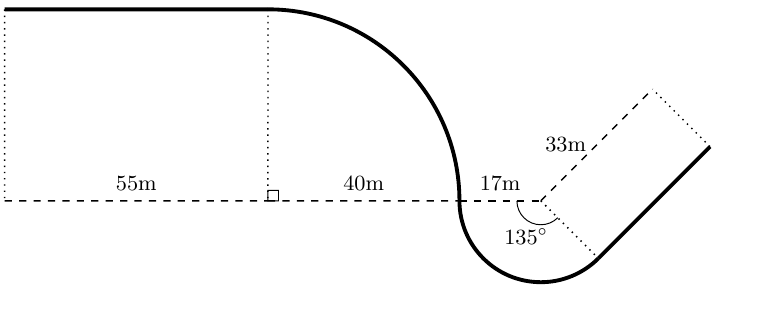
\includegraphics[scale=1]{es1-5-3}
		
		\begin{tikzpicture}[scale=0.7]
		\tkzDefPoint(0,0){O}
		\tkzDefPoint(-5.7,0){O1}
		\tkzDefShiftPoint[O](-1.7,0){P3}
		\tkzDefShiftPoint[P3](-4,4){P2}
		\tkzDefShiftPoint[P2](0,-4){P2a}
		\tkzDefShiftPoint[P2](-5.5,0){P1}
		\tkzDefShiftPoint[P1](0,-4){P1a}
		\tkzDefShiftPoint[O](-45:1.7){P4}
		\tkzDefShiftPoint[P4](45:3.3){P5}
		\tkzDefShiftPoint[P5](135:1.7){P5a}
		\tkzDrawSegments[ultra thick,color=black](P1,P2 P4,P5)
		\tkzDrawArc[ultra thick,color=black](O,P3)(P4)
		\tkzDrawArc[ultra thick,color=black](O1,P3)(P2)
		\tkzDrawSegments[dashed,color=black](P1a,P2a   P2a,P3 P3,O  O,P5a)
		\tkzDrawSegments[dotted,color=black](P1,P1a P2,P2a  O,P4  P5,P5a)
		\tkzLabelSegment(P1a,P2a){\footnotesize $55$m}
		\tkzLabelSegment(P3,P2a){\footnotesize  $40$m}
		\tkzLabelSegment(P3,O){\footnotesize  $17$m}
		\tkzLabelSegment[left](O,P5a){\footnotesize $33$m}
		\tkzMarkAngle[arc=l,size=0.5 cm,](P3,O,P4)
		\tkzLabelAngle[pos=0.8,circle](P3,O,P4){\footnotesize  $135^\circ$}
		\tkzMarkRightAngle(P2,P2a,P3)
		\end{tikzpicture}
		%TODO diegno in tikz

	}
	
	\solonly{$\SI{190.89}{\meter}$}
	
	%%%%%%%%%%%%%%%%%%%%%%%%%%%%%%%%%%%%%%%%%%%%%%%%%%%%%%%%%%%%%%%
	%\exonly{\columnbreak}
	%\question
	%\exonly{
	%\FR{
	%Sur le schéma ci-dessous, en noir est représenté la plan d'une route. Calculer la longueur du virage. Le virage a un rayon de courbure de \SI{122}{\meter}.
	%}
	%\DE{}
	%
	%
	%
	%\begin{tikzpicture}%[scale=.8]
	%\tkzDefPoint(0,0){O}
	%\tkzDefShiftPoint[O](0,3){P2}
	%\tkzDefShiftPoint[P2](-3,0){P1}
	%\tkzDefShiftPoint[O](30:3){P3}
	%\tkzDefShiftPoint[P3](-60:2){P4}
	%\tkzDrawSegments[ultra thick,color=black](P1,P2 P3,P4)
	%\tkzDrawArc[ultra thick,color=black](O,P3)(P2)
	%\tkzInterLL(P1,P2)(P3,P4)  \tkzGetPoint{I}
	%\tkzDrawSegments[dashed,color=black](P2,I I,P4)
	%\tkzMarkAngle[arc=l,size=0.5 cm,](P3,I,P2)
	%\tkzLabelAngle[pos=0.8,circle](P2,I,P3){$240^\circ$}
	%%\tkzLabelSegment[left](O,P5a){$33$m}
	%%\tkzMarkAngle[arc=l,size=0.5 cm,](P3,O,P4)
	%%\tkzLabelAngle[pos=-0.8,circle](P3,O,P4){$135^\circ$}
	%%\tkzMarkRightAngle(P2,P2a,P3)
	%\end{tikzpicture}
	%}
	%
	%\solonly{$\SI{129.76}{\meter}$}
	%
	%
	%%%%%%%%%%%%%%%%%%%%%%%%%%%%%%%%%%%%%%%%%%%%%%%%%%%%%%%%%
	%\question
	%\exonly{
	%\FR{
	%Paris et Niamey, la capitale du Niger, sont sur le même méridien. Paris a une latitude de \ang{45;52;} et Niamey une latitude de \ang{13;31;}. Sachant que la terre a un diamètre approximatif de \SI{12800}{\kilo\meter}, calculer la distance entre les deux villes. Faire un croquis de la situation.
	%}
	%}
	%
	%\solonly{\SI{3613.53}{\kilo\meter}}
	%
	%
	%\question
	%\exonly{
	%\FR{
	%Calculer l'aire d'un secteur circulaire (de rayon \SI{11}{\centi\meter}) dont l'angle au centre mesure:
	%}
	%\DE{
	%
	%}}
	%
	%\begin{parts}
	%\part
	%\exonly{\ang{55}} \solonly{\SI{58.08}{\square\centi\meter}}
	%
	%\part
	%\exonly{$\dfrac{\pi}{5}$ \SI{}{\radian}} \solonly{\SI{38.01}{\square\centi\meter}}
	%
	%\end{parts}
	
	
	%%%%%%%%%%%%%%%%%%%%%%%%%%%%%%%%%%%%%%%%%%%%%%%%%%%%%%%%%%%%%%%%%%%%%%%%
	\question
	\exonly{
		I rettangoli  $R_1$, $R_2$, $R_3$ e $R_4$ hanno la stessa superficie.
		
		Calcolare l'area e il perimetro della figura.
		
		%TODO : convert in TikZ
		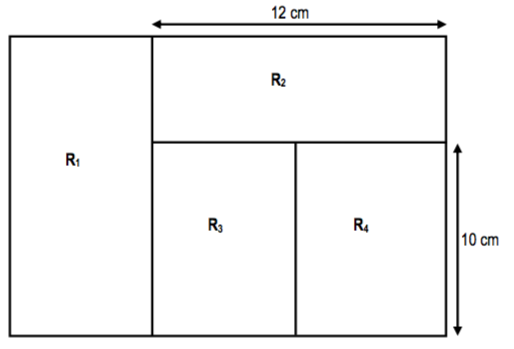
\includegraphics[width=0.5\linewidth]{surf-1}
	}
	
	\solonly{
		$A=\SI{240}{\square\centi\meter}$ \\
		$P=\SI{62}{\centi\metre}$
	}
	
	%%%%%%%%%%%%%%%%%%%%%%%%%%%%%%%%%%%%%%%%%%%%%%%%%%%%%%%%%%%%%%%%%%%%%%%%
	%
	%\question
	%\exonly{
	%\FR{
	%$ABCD$ est un rectangle et $M$ est le milieu de $CD$. L'aire du triangle $\Delta_2$ a $\SI{4}{\square\centi\meter}$ de plus que l'aire du triangle $\Delta_1$. Calculez l'aire du triangle grisé.
	%}
	%
	%\includegraphics[width=\linewidth]{surf-2}
	%}
	%
	%\solonly{
	%$\FR{A}\DE{F}=\SI{25.5}{\square\centi\meter}$
	%}
	%
	%%%%%%%%%%%%%%%%%%%%%%%%%%%%%%%%%%%%%%%%%%%%%%%%%%%%%%%%%%%%%%%%%%%%%%%%
	
	
	%\question
	%\exonly{
	%\FR{
	%On considère un parallélogramme $ABCD$. Son périmètre vaut $\SI{25.2}{\centi\meter}$ et le côté $AB$ est deux fois plus grand que le côté $BC$. La somme des longueurs des deux hauteurs de ce parallélogramme donne $\SI{12}{\centi\meter}$. Calculez la surface de ce parallélogramme.
	%}}
	%\solonly{
	%$\FR{A}\DE{F}=\SI{33.6}{\square\centi\meter}$
	%}
	%%%%%%%%%%%%%%%%%%%%%%%%%%%%%%%%%%%%%%%%%%%%%%%%%%%%%%%%%%%%%%%%%%%%%%%%
	
	%\question
	%\exonly{
	%\FR{
	%Le périmètre d’un losange vaut  $\SI{42}{\centi\meter}$. Le rayon du cercle inscrit à ce losange vaut  $\SI{3.2}{\centi\meter}$. Calculez l'aire du losange.
	%}}
	%\solonly{
	%$\FR{A}\DE{F}=\SI{67.2}{\square\centi\meter}$
	%}
	
	%%%%%%%%%%%%%%%%%%%%%%%%%%%%%%%%%%%%%%%%%%%%%%%%%%%%%%%%%%%%%%%%%%%%%%%%
\exnewpage
	\question
	\exonly{
		Calcolare l'area della superficie in grigio. 
		Il lato del quadrato misura $\SI{10}{\centi\meter}$.
		$A$ e $B$ sono i centri degli archi di cerchio.
		
		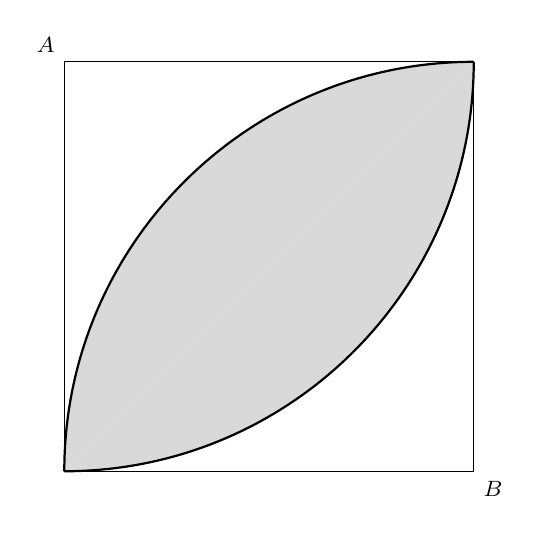
\begin{tikzpicture}[scale=1.3]
		\filldraw[gray!30] (4,0) arc (90:180:4) ;
		\filldraw[gray!30] (4,0) arc (0:-90:4);
		\draw (0,0) node[above left] {$A$} rectangle (4,-4) node[below right] {$B$};
		\draw[thick] (4,0) arc (90:180:4);
		\draw[thick] (4,0) arc (0:-90:4);
		\end{tikzpicture}
		%\includegraphics[width=0.6\linewidth]{surf-3}
	}
	
	
	\solonly{
		$A\approx\SI{57.08}{\square\centi\meter}$
	}
	
	%%%%%%%%%%%%%%%%%%%%%%%%%%%%%%%%%%%%%%%%%%%%%%%%%%%%%%%%%%%%%%%%%%%%%%%%
	%
	%\question 
	%\exonly{
	%\FR{Soient $C_1$ et $C_2$  deux cercles tangents en $B$. Le rayon $r_1$ mesure $\SI{4.5}{\centi\meter}$ et $\alpha= 60^{\circ}$. $t$ est la tangente commune aux deux cercles.}}
	%
	%\begin{parts}
	%\part
	%\exonly{\FR{
	%	Calculez le rayon $r_2$.
	%}} \solonly{$r_2=\SI{1.5}{\centi\meter}$}
	%
	%\part
	%\exonly{\FR{
	%	Calculez l'aire de la surface grisée.
	%}} \solonly{$A\approx\SI{2.64}{\square\centi\meter}$}
	%
	%\end{parts}
	%
	%\exonly{
	%\includegraphics[width=\linewidth]{surf-4}
	%}
	%
	
	%%%%%%%%%%%%%%%%%%%%%%%%%%%%%%%%%%%%%%%%%%%%%%%%%%%%%%%%%%%%%%%%%%%%%%%%
	
	\question 
	\exonly{
		Calcolare l'area della superficie in grigio.
		Il lato del quadrato misura $\SI{7}{\centi\meter}$.
		$A$ e $B$ sono i centri degli archi di cerchio.
	}
	
	\exonly{
		
		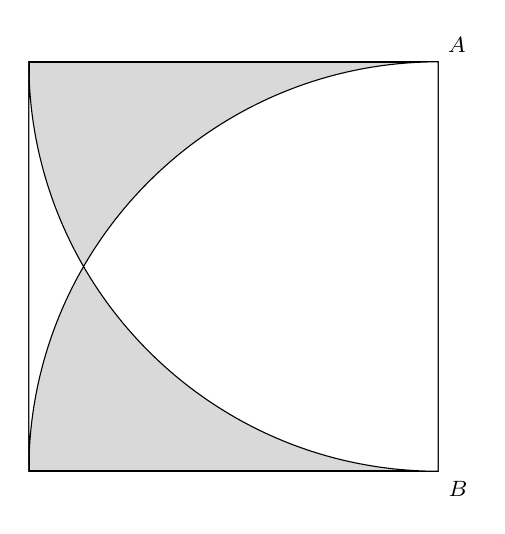
\begin{tikzpicture}[scale=1.3]
		\path (4,0) node[above right] {$A$} ;
		\filldraw[thick,draw=black,fill=gray!30] (0,0) rectangle (4,-4) node[below right] {$B$};
		
		\clip (0,0) rectangle (4,-4);
		\begin{scope}
		\filldraw[draw=black,fill=white,even odd rule] (0,0) rectangle (4,-4) (4,-4) circle (4) (4,0) circle (4) ;
		\end{scope}
		
		\end{tikzpicture}
		
		%\includegraphics[width=0.6\linewidth]{surf-5}
	}
	
	\solonly{
		$A\approx\SI{16.76}{\square\centi\meter}$
	}
	
	%%%%%%%%%%%%%%%%%%%%%%%%%%%%%%%%%%%%%%%%%%%%%%%%%%%%%%%%%%%%%%%%%%%%%%%%
	
	\question 
	\exonly{
		L'arco di cerchio (di centro $O$) qui sotto ha un angolo al centro di \ang{230}.
		La lunghezza della corda $AB$ é di $\SI{7}{\meter}$.
		
		Calcolare il raggio $R$ dell'arco di cerchio e l'altezza $H$.}
	
	\exonly{
		\begin{tikzpicture}[scale=0.8]
		\draw (0,0) node[above] {$O$} -- node[above, midway] {$R$} (15:4);
		\draw (-45:4) node[below] {$B$} arc (-45:225:4) node[below] {$A$};
		\draw (-45:4) --  + (0:2) -- +(180:8);
		\draw[dashed] (-45:4) ++(0:1.5) |- (0,4);
		\coordinate (A) at ({$(-45:4)+(0:1.5)$} |- {$(0,4)$});
		\draw[latex-latex, thick] (-45:4) ++(0:1.5) -- node[right,midway]{$H$}(A);
		
		\end{tikzpicture}
		
		
		%\includegraphics[width=\linewidth]{surf-6}
	}
	
	\solonly{
		$R\approx\SI{3.86}{\meter}$ , $H\approx\SI{5.49}{\meter}$
	}
	
	
\end{questions}



%%%%%%%%%%%%%%%%%%%%%%%%%%%%%%%%%%%%%%%%%%%%%%%%%%%%%%%%%%%%%%%

\end{questions}
\section{Geometria dello spazio}
\subsection{Prismi e piramidi}
\begin{questions}

	\begin{qblock}
		\question
		\exonly{
			Consideriamo la  piramide di base $ABC$ e vertice $S$.
			I lati  $SA$, $SB$ e $SC$ sono perpendicolari tra loro e misurano rispettivamente \SI{1}{\metre}, \SI{2}{\metre}  e \SI{3}{\metre}.}


		\ifprintanswers   \else
		
		\begin{center}
				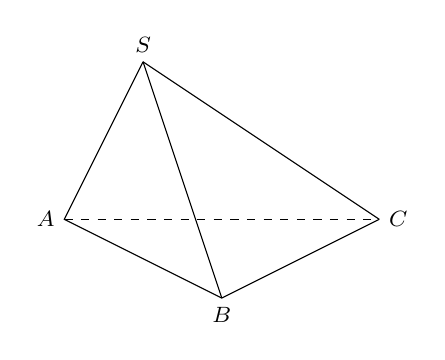
\begin{tikzpicture}
					\draw
					(0,0) coordinate [label=left:$A$] (A)
					(4,0) coordinate [label=right:$C$]  (C) --
					(2,-1) coordinate [label=below:$B$]  (B) -- (A) --
					(1,2) coordinate [label=above:$S$]  (S) edge (C)	 edge (B);
					\draw[dashed] (A) -- (C);
				\end{tikzpicture}
		\end{center}
		\fi


		\begin{parts}
			\part
			\exonly{
				Determinare l'area della base $ABC$.
				%	Déterminer l’aire de la base $ABC$ de cette pyramide.
			}
			\solonly{\SI{3.5}{\square\metre}}
			\part
			\exonly{
				Determinare il volume di questa piramide.
				%	Déterminer le volume de cette pyramide.
			}
			\solonly{\SI{1}{\cubic\metre}}
		\end{parts}
	\end{qblock}

	\begin{qblock}
		\question
		\exonly{
			I vertici di un cubo di lato \SI{10}{\centi\metre} vengono tagliati affinché le facce del cubo diventino degli ottagoni regolari.
		}

		\begin{parts}
			\part
			\exonly{
				Disegnare uno schizzo della situazione.
				%	Faire un croquis de la situation.
			}

			\ifprintanswers
				\begin{tikzpicture}[baseline={($(current bounding box.north)-(0,1.6ex)$)},scale=0.6]
					%\tikzstyle{isometric}=[x={(0.710cm,-0.410cm)},y={(0cm,0.820cm)},z={(-0.710cm,-0.410cm)}]
					\tikzset{every path/.style={isometric}}
					\tikzset{face/.style={fill=gray!20}}
					\pgfmathsetmacro{\cubex}{4}
					\pgfmathsetmacro{\cubey}{4}
					\pgfmathsetmacro{\cubez}{4}
					\pgfmathsetmacro{\ratio}{1/3}

					\coordinate (FTR) at (0,0,0);
					\coordinate (FTL) at (-\cubex,0,0);
					\coordinate (FBL) at (-\cubex,-\cubey,0);
					\coordinate (FBR) at (0,-\cubey,0);
					\coordinate (BTR) at (0,0,-\cubez);
					\coordinate (BBR) at (0,-\cubey,-\cubez);
					\coordinate (BTL) at (-\cubex,0,-\cubez);
					\coordinate (BBL) at (-\cubex,-\cubey,-\cubez);


					\draw[dotted] (FBL) -- (BBL);

					\shadedraw[face] ($(FTR)!\ratio!(FTL)$) -- ($(FTL)!\ratio!(FTR)$) -- ($(FTL)!\ratio!(FBL)$) -- ($(FBL)!\ratio!(FTL)$) --
					($(FBL)!\ratio!(FBR)$) -- ($(FBR)!\ratio!(FBL)$) --
					($(FBR)!\ratio!(FTR)$) -- ($(FTR)!\ratio!(FBR)$) --cycle;
					%top face
					\shadedraw[face] ($(FTR)!\ratio!(FTL)$) -- ($(FTR)!\ratio!(BTR)$) -- ($(BTR)!\ratio!(FTR)$) -- ($(BTR)!\ratio!(BTL)$) --
					($(BTR)!\ratio!(BTL)$) -- ($(BTL)!\ratio!(BTR)$) --
					($(BTL)!\ratio!(FTL)$) --  ($(FTL)!\ratio!(BTL)$)
					-- ($(FTL)!\ratio!(FTR)$) --cycle;
					%right face
					\shadedraw[face] ($(FTR)!\ratio!(BTR)$) -- ($(BTR)!\ratio!(FTR)$) -- ($(BTR)!\ratio!(BBR)$) -- ($(BBR)!\ratio!(BTR)$) --
					($(BBR)!\ratio!(FBR)$) -- ($(FBR)!\ratio!(BBR)$) --
					($(FBR)!\ratio!(FTR)$) --  ($(FTR)!\ratio!(FBR)$)
					-- ($(FTR)!\ratio!(FBR)$) -- cycle;

					%top right corner
					\shadedraw[face] ($(FTR)!\ratio!(BTR)$) -- ($(FTR)!\ratio!(FTL)$) -- ($(FTR)!\ratio!(FBR)$) --cycle;
					%top left corner
					\shadedraw[face] ($(FTL)!\ratio!(BTL)$) -- ($(FTL)!\ratio!(FTR)$) -- ($(FTL)!\ratio!(FBL)$) --cycle;

					%bottom right corner
					\shadedraw[face] ($(FBR)!\ratio!(FTR)$) -- ($(FBR)!\ratio!(FBL)$) -- ($(FBR)!\ratio!(BBR)$) --cycle;

					%top right corner
					\shadedraw[face] ($(BTR)!\ratio!(FTR)$) -- ($(BTR)!\ratio!(BTL)$) -- ($(BTR)!\ratio!(BBR)$) --cycle;
					%\fill[red] (0,0,0) circle (2pt);
					\draw[dotted] (FTR)  -- (FTL)  -- (FBL)  -- (FBR)  -- cycle;
					\draw[dotted] (FTR) -- (BTR)  -- (BTL)  -- (FTL) -- cycle;
					\draw[dotted] (FTR) -- (FBR) -- (BBR)  -- (BTR) -- cycle;
				\end{tikzpicture}
			\fi
			\part
			\exonly
			{
				Calcolare l'area esterna totale del solido ottenuto.
				%	Calculer l’aire extérieure totale du corps ainsi obtenu
			}
			\solonly{\SI{556.42}{\square\centi\metre}}
			\part
			\exonly{
				Calcolarne il volume.
				%	Calculer son volume.
			}
			\solonly{\SI{966}{\cubic\centi\metre}}
		\end{parts}
	\end{qblock}

	\begin{qblock}
		\question
		\exonly{
			Calcolare l'altezza della piramide retta a base rettangolare $ABCD$ il cui vertice é $S$.
			Le misure seguenti sono conosciute: $AB$=\SI{20}{\centi\metre}, $BC$=\SI{23}{\centi\metre} e $AS$=\SI{32}{\centi\metre}.
		}

		\ifprintanswers   \else
			
			\begin{center}
				\begin{tikzpicture}[scale=0.7]
					\coordinate[label=left:$A$] (A) at (0,0);
					\coordinate[label=right:$B$] (B) at (4,0);
					\coordinate[label=below:$C$] (C) at ($(B)+(35:3)$);
					\coordinate[label=below:$D$] (D) at ($(A)+(35:3)$);
					\draw (A)-- (B)--(C)--(D)-- cycle;
					\draw (3,5) coordinate [label=above:$S$]  (S)  edge (A) edge (D) edge (C)	 edge (B);
	
				\end{tikzpicture}
			\end{center}
		\fi
		\solonly{\SI{28.14}{\centi\metre}}
	\end{qblock}

	\begin{qblock}
		\question
		\exonly{
			Da uno degli spigoli di un cubo tagliamo un tetraedro i cui spigoli misurano  $AP=AQ=$\SI{3}{\centi\metre} e $AR=$\SI{4}{\centi\metre}.
		}

		
		\begin{center}
			\begin{tikzpicture}[baseline={($(current bounding box.north)-(0,1.6ex)$)}]
				%\tikzstyle{isometric}=[x={(0.710cm,-0.410cm)},y={(0cm,0.820cm)},z={(-0.710cm,-0.410cm)}]
				%\tikzset{every path/.style={isometric}}
				\tikzset{face/.style={fill=gray!20}}
				\pgfmathsetmacro{\cubex}{2}
				\pgfmathsetmacro{\cubey}{2}
				\pgfmathsetmacro{\cubez}{2}
				\pgfmathsetmacro{\ratio}{1/3}
	
				\coordinate (FTR) at (0,0,0);
				\coordinate[label=left:$A$] (FTL) at (-\cubex,0,0);
				\coordinate (FBL) at (-\cubex,-\cubey,0);
				\coordinate (FBR) at (0,-\cubey,0);
				\coordinate (BTR) at (0,0,-\cubez);
				\coordinate (BBR) at (0,-\cubey,-\cubez);
				\coordinate (BTL) at (-\cubex,0,-\cubez);
				\coordinate (BBL) at (-\cubex,-\cubey,-\cubez);
				\coordinate[label=left:$R$] (R) at ($(FTL)!0.6!(BTL)$);
				\coordinate[label=left:$Q$] (Q) at ($(FTL)!0.6!(FBL)$);
				\coordinate[label=right:$P$] (P) at ($(FTL)!0.6!(FTR)$);
	
				\draw[dotted] (FTR)  -- (FTL)  -- (FBL)  -- (FBR)  -- cycle;
				\draw[dotted] (FTR) -- (BTR)  -- (BTL)  -- (FTL) -- cycle;
				\draw[dotted] (FTR) -- (FBR) -- (BBR)  -- (BTR) -- cycle;
				\draw[very thick] (FTL) -- (R) -- (P) -- (Q) --cycle;
				\draw[very thick]  (FTL) -- (Q) -- (P);
				\draw[very thick, dashed]  (R) -- (Q);
			\end{tikzpicture}
		\end{center}

		\begin{parts}
			\part
			\exonly{
				Calcolare il volume del tetraedro.
				%Calculer le volume du tétraèdre.
			}
			\solonly{\SI{6}{\cubic\centi\metre}}

			\part
			\exonly{
				Calcolare l'altezza del tetraedro rispetto alla base $PQR$.
				%Calculer la hauteur du tétraèdre relative à la base $PQR$.
			}
			\solonly{\SI{1.9}{\centi\metre}}
		\end{parts}
	\end{qblock}

	\begin{qblock}
		\question
		\exonly{
			Un prisma a base quadrata di lato $b=\SI{2}{\centi\metre}$ é inscritto in una piramide regolare a base quadrata di lato $a=\SI{6}{\centi\metre}$ e altezza $h=\SI{10}{\centi\metre}$.

		}


		\begin{parts}
			\part
			\exonly{
				Eseguire uno schizzo della situazione.
				%Faire un croquis de la situation.
			}
			\ifprintanswers
				\begin{tikzpicture}[baseline={($(current bounding box.north)-(0,1.6ex)$)},scale=0.4]
					%\tikzstyle{isometric}=[x={(0.710cm,-0.410cm)},y={(0cm,0.820cm)},z={(-0.710cm,-0.410cm)}]
					%\tikzset{every path/.style={isometric}}
					\tikzset{face/.style={fill=gray!20}}
					\pgfmathsetmacro{\cubex}{4}
					\pgfmathsetmacro{\cubey}{4}
					\pgfmathsetmacro{\cubez}{4}
					\pgfmathsetmacro{\ratio}{1/2}
					\pgfmathsetmacro{\shift}{-3.5cm}

					\coordinate (S) at (0,7,0);
					\coordinate (FL) at (-\cubex,0,\cubez);
					\coordinate (FR) at (\cubex,0,\cubez);
					\coordinate (BR) at (\cubex,0,-\cubez);
					\coordinate (BL) at (-\cubex,0,-\cubez);
					\coordinate (PFTR) at ($(FR)!\ratio!(S)$);
					\coordinate (PFTL) at ($(FL)!\ratio!(S)$);
					\coordinate (PBTL) at ($(BL)!\ratio!(S)$);
					\coordinate (PBTR) at ($(BR)!\ratio!(S)$);
					\coordinate (PFBR) at ([yshift=\shift] PFTR);
					\coordinate (PFBL) at ([yshift=\shift] PFTL);
					\coordinate (PBBL) at ([yshift=\shift] PBTL);
					\coordinate (PBBR) at ([yshift=\shift] PBTR);


					\draw (FL) -- (FR) -- (BR);
					\draw[dotted] (BR) -- (BL) --(FL);
					\draw (S) edge (FR)  edge (FL) edge (BR);
					\draw[dotted] (S)  edge (BL) ;

					\draw[thick] (PFTL) -- (PFTR) -- (PBTR) --(PBTL) -- cycle;
					\draw[thick] (PFBR) -- (PFBL) -- (PBBL) -- (PBBR) -- cycle;
					\draw[thick] (PFTL) -- (PFBL) (PFTR) -- (PFBR) (PBTL) --(PBBL) (PBTR)--(PBBR);

				\end{tikzpicture}
			\fi
			\part
			\exonly{
				Calcolare il volume del prisma.
				%Calculer le volume du prisme.

			}
			\solonly{\SI{26.67}{\cubic\centi\metre}}
		\end{parts}
	\end{qblock}

	\begin{qblock}
		\question
		\exonly{
			I vertici di un tetraedro di lato \SI{12}{\centi\metre} vengono tagliati affinché le facce del tetraedro divengano degli esagoni regolari.

			Determinare il volume del solido ottenuto.
			%Déterminer le volume du corps ainsi obtenu.
		}
		\solonly{\SI{173.48}{\cubic\centi\metre}}

		
		\begin{center}
			\begin{tikzpicture}[scale=2]
				\tikzset{every path/.style={isometric}}
				\pgfmathsetmacro{\a}{2/ sqrt(3)}
				\pgfmathsetmacro{\b}{sqrt(3)/2}
				\pgfmathsetmacro{\h}{sqrt(23/4)}
				\pgfmathsetmacro{\ratio}{1/3}
				\pgfmathsetmacro{\Ratio}{2/3}
	
				\coordinate (A) at ( 0,0,\a);
				\coordinate (B) at ( 1,0,-\b);
				\coordinate (C) at ( -1,0,-\b);
				\coordinate (S) at ( 0,\h,0);
				\draw[dotted] (A)--(B);
	
				\draw[dotted] (C) edge (B) edge (A);
				\draw[dotted] (S) edge (A) edge (B);
				\draw [dotted]  (S) edge (C);
	
				\shadedraw[dashed] ($(A)!\Ratio!(S)$) -- ($(B)!\Ratio!(S)$) -- ($(C)!\Ratio!(S)$) -- cycle;
				\draw ($(A)!\Ratio!(S)$) -- ($(B)!\Ratio!(S)$) ;
	
				\shadedraw[dashed] ($(A)!\ratio!(S)$) -- ($(A)!\ratio!(B)$) -- ($(A)!\ratio!(C)$) --cycle;
				\draw ($(A)!\ratio!(S)$) -- ($(A)!\ratio!(B)$);
	
				\shadedraw[dashed] ($(B)!\ratio!(S)$) -- ($(B)!\ratio!(A)$) -- ($(B)!\ratio!(C)$) --cycle;
				\draw ($(B)!\ratio!(S)$) -- ($(B)!\ratio!(A)$);
	
				\draw[dashed] ($(C)!\ratio!(S)$) -- ($(C)!\ratio!(A)$) -- ($(C)!\ratio!(B)$) --cycle;
	
				\shade ($(A)!\Ratio!(S)$) -- ($(B)!\Ratio!(S)$) -- ($(B)!\ratio!(S)$) -- ($(B)!\ratio!(A)$)--($(B)!\Ratio!(A)$) -- ($(A)!\ratio!(S)$) --cycle;
	
			\end{tikzpicture}
		\end{center}
	\end{qblock}

\end{questions}

\subsection{Solidi di rotazione}
\begin{questions}

	\begin{qblock}
		\question
		\exonly{
			Il rapporto tra l'apotema e il diametro di un cono retto é di $\frac{5}{6}$ (vale a dire che $\frac{l}{d}=\frac{5}{6}$).\\
			Il volume del cono é di \SI{2.7}{\cubic\centi\metre}.\\
			Calcolare la superficie laterale del cono.\\
		}
		\solonly{\SI{8.13}{\square\centi\metre}}
	\end{qblock}


	\begin{qblock}
		\question
		\exonly{
			Pratichiamo un foro circolare di \SI{10}{\centi\metre}  di diametro in una placca metallica.

			Disponiamo nel foro una sfera di raggio $R>\SI{5}{\centi\metre} $ e constatiamo che la parte visibile della sfera ha un'altezza di \SI{13}{\centi\metre}.

		}

		\begin{parts}
			\part
			\exonly{
				Eseguire uno schizzo della situazione.

			}
			\ifprintanswers
				\begin{tikzpicture}[scale=0.5,baseline={($(current bounding box.north)-(0,1.6ex)$)}]
					\pgfmathsetmacro{\radius}{3}
					\pgfmathsetmacro{\planex}{5}
					\pgfmathsetmacro{\planez}{2.5}
					\pgfmathsetmacro{\ang}{30}
					\draw (-\planex,{-sin(\ang)*\radius},\planez) -- (-\planex,{-sin(\ang)*\radius},-\planez) -- (\planex,{-sin(\ang)*\radius},-\planez)--(\planex,{-sin(\ang)*\radius},\planez);
					\shadedraw[shading=ball,ball color=gray!10] (0,0) circle (\radius cm);
					\draw[very thick] (0,{-sin(\ang)*\radius}) ellipse ({cos(\ang)*\radius} and 0.5);
					\draw[very thick] (\planex,{-sin(\ang)*\radius},\planez) -- (-\planex,{-sin(\ang)*\radius},\planez) ;
					\draw [dashed] (-0.7*\planex,{-sin(\ang)*\radius}) |- (0,\radius);
					\draw[latex-latex] (-0.7*\planex,{-sin(\ang)*\radius}) -- node[left] {\SI{13}{\centi\metre}} ({$(-0.7*\planex,{-sin(\ang)*\radius})$} |- {$(0,\radius)$});

					\draw[dashed] ({cos(\ang)*\radius},{-sin(\ang)*\radius}) -- ({cos(\ang)*\radius},-4) -|  ({-cos(\ang)*\radius},{-sin(\ang)*\radius});
					\draw[latex-latex] ({cos(\ang)*\radius},-4) -- node[below] {\SI{10}{\centi\metre}}({-cos(\ang)*\radius},-4);
				\end{tikzpicture}

			\fi




			\part

			\exonly{
				Determinare il volume della sfera.

			}
			\sol{\SI{1.74}{\cubic\deci\metre}}
		\end{parts}
	\end{qblock}



	\begin{qblock}
		\question
		\exonly{
			Vogliamo costruire una boa avente la forma di un settore sferico in modo che la superficie della calotta sia identica alla superficie laterale del cono.

		}

		\begin{parts}
			\part

			\exonly{
				Calcolare il raggio $r$ della calotta e il volume $V$ del settore sferico se $R=\SI{70}{\centi\metre}$
			}
			\solonly{$r=\SI{56}{\centi\metre}$ , $h=\SI{28}{\centi\metre}$ e \\ $V=\SI{287351}{\cubic\centi\metre}$}
			\part
			\exonly{
				Calcolare il raggio $r$ della calotta e il volume $V$ del settore sferico in funzione del raggio $R$ della sfera da cui viene estratto.}
			\solonly{
				$r=\dfrac{4}{5}R$ e $V=\dfrac{4}{15}\pi R^3$
			}

		\end{parts}

		\ifprintanswers   \else
		\begin{center}
			\begin{tikzpicture}[baseline={($(current bounding box.north)-(0,1.6ex)$)},scale=0.6]
				\pgfmathsetmacro{\radius}{3}
				\pgfmathsetmacro{\planex}{5}
				\pgfmathsetmacro{\planez}{2.5}
				\pgfmathsetmacro{\ang}{30}
				\pgfmathsetmacro{\err}{0.1}
				\coordinate (O) at (0,0);
				\draw[] (O) circle (\radius cm);
				%manteau secteur spherique
				\shadedraw[gray!10, color=black] ({cos(\ang)*\radius-\err},{sin(\ang)*\radius-\err}) -- (O) node [below] {$O$} -- node[below] {$R$} ({-cos(\ang)*\radius+\err},{sin(\ang)*\radius-\err});
	
				\shadedraw[thick] ({cos(\ang)*\radius},{sin(\ang)*\radius}) arc (0:-180:{cos(\ang)*\radius} and 0.4) arc (180-\ang:\ang:\radius);
	
				\shadedraw[very thick] ({cos(\ang)*\radius},{sin(\ang)*\radius}) arc (\ang:180-\ang:\radius);
	
				\draw[dotted]  ({cos(\ang)*\radius},{sin(\ang)*\radius}) arc (0:180:{cos(\ang)*\radius} and 0.4);
	
				\draw[dashed] (0,{sin(\ang)*\radius} ) -- node [above] {$r$} ({cos(\ang)*\radius},{sin(\ang)*\radius});
				\draw [dashed] (0,\radius + 1) -- (0, -\radius -1);
			\end{tikzpicture}
		\end{center}
		\fi
	\end{qblock}


	\begin{qblock}
		\question
		\exonly{
			In una sfera di raggio $R=\SI{1}{\metre}$ é inscritto un cilindro la cui superficie laterale vale la metà della superficie della sfera.

			Calcolare il volume del cilindro.
		}

		\ifprintanswers   \else
		\begin{center}
			\begin{tikzpicture}[baseline={($(current bounding box.north)-(0,1.6ex)$)},scale=2]
				\pgfmathsetmacro{\Radius}{1}
				\pgfmathsetmacro{\radius}{1/sqrt(2)}
				\pgfmathsetmacro{\height}{sqrt(2) /2 }
	
				\coordinate (O) at (0,0);
				\shadedraw[shading=ball,ball color=gray!10] (O) circle (\Radius);
				\draw (0,\height  ) ellipse ({\radius}  and 0.1);
				\draw(0,-\height ) ellipse ({\radius}  and 0.1);
				\draw[dotted] (O) ellipse ({\Radius} and 0.1);
				\draw (-\radius, \height) -- (-\radius,- \height);
				\draw (\radius, \height) -- (\radius, -\height);
				\draw[dashed] (0,\height + 0.5) -- (0,-\height -0.5);
				\draw[thick] (O) -- node[above] {$R$} (\Radius,0);
				%manteau secteur spherique
			\end{tikzpicture}
		\end{center}

		\fi


		\solonly{$V=\SI{2.2}{\cubic\metre}$}
	\end{qblock}


	\begin{qblock}
		\question
		\exonly{
			Calcolare il volume di un cono retto di altezza $h=\SI{15}{\centi\metre}$ nel quale é inscritta una sfera di raggio $r=\SI{6}{\centi\metre}$.
		}
		\solonly{\SI{2827.4}{\cubic\centi\metre}}

		\ifprintanswers   \else
		\begin{center}
			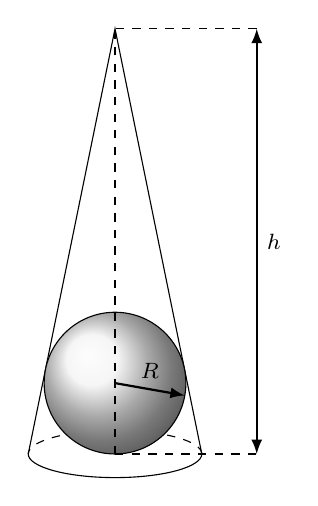
\begin{tikzpicture}[scale=0.3]
				\pgfmathsetmacro\radius{9/sqrt(6)}
				\coordinate (a) at (0,\radius);
				\coordinate (b) at (0,18);
				\draw (\radius,0) -- (b) -- (-\radius,0);
				\draw (\radius,0) arc(0:-180:{\radius} and 1);
				\draw[dashed] (\radius,0) arc(0:180:{\radius} and 1);
				%\fill[black] (0,0) circle (2pt) node[below left] { $O_1$};
	
	
				\shadedraw[shading=ball,ball color=gray!10] (0,3) circle (3);
				\draw[-latex,thick] (0,3) -- ++(-10:3) node[midway,above] {$R$};
	
				\draw[dashed] (0,0) -- (0,18);
				\draw[dashed] (0,0) -- (6,0)  (6,18) --(0,18);
				\draw[latex-latex,thick] (6,18) -- (6,0) node[midway, right] {$h$};
			\end{tikzpicture}
		\end{center}
		\fi
	\end{qblock}


	\begin{qblock}
		\question
		\exonly{
			Una sfera di raggio $R$  é illuminata da una sorgente luminosa puntiforme situata ad una distanza $L$ dal centro $O$ della sfera.
		}

		\begin{parts}
			\part

			\exonly{
				Calcolare la porzione (in \%) di superficie non illuminata della sfera se
				$R=\SI{1}{\metre}$ e $L=\SI{2.5}{\metre}$}
			\solonly{$70\%$}

			\part
			\exonly{
				Calcolare la proporzione si superficie non illuminata della sfera in funzione di $R$ e $L$.}

			\solonly{$\dfrac{(L+R)}{2L}$}
			\part
			\exonly{
				Discutere i due casi estremi $L \gg R$ (che potrebbe modellizzare la situazione Terra-Sole) e $L\approx R$.}
			\solonly{$50\%$ e $0\%$}

		\end{parts}



		\ifprintanswers   \else
			
			\begin{center}
				\begin{tikzpicture}
					\node[circle, draw, very thick] (c) at (0, 0) [minimum size=3cm] {};
					\fill[red]   (4, 0) coordinate (a) circle (3pt);
					\draw (tangent cs:node=c, point={(a)}, solution=1) coordinate (t1)-- (a);
					\draw (tangent cs:node=c, point={(a)}, solution=2) coordinate (t2)-- (a);
					%\draw[dashed] (0,0) -- (t1);
					%\draw[dashed] (0,0) -- (t2);
					\fill[gray!10] (t1)  let \p1 = ($ (0,0) - (t1) $) in  arc ({atan(\y1/\x1)}:{360-atan(\y1/\x1)}:1.5);
	
	
					\path ($(t1)!0.5!(t2)$) coordinate (e1);
	
					\fill[gray!10] (e1)  let \p1 = ($ (t2) - (t1) $) in  ellipse (0.2 cm and {0.5*veclen(\x1,\y1)});
					\node[circle, draw, very thick] (c) at (0, 0) [minimum size=3cm] {};
					\draw (t1) let \p1 = ($ (t1) - (t2) $) in
					arc (90:-90: 0.2 cm and {0.5*veclen(\x1,\y1)});
					\draw (0,0) -- node[below left] {$R$} (150:1.5);
					\fill (0,0) circle (1pt) node [below] {$O$};
					\draw [dashed] (0,0) -- (0,-2) -| (a);
					\draw [latex-latex] (0,-2) -- node [above] {$L$}({$(0,-2)$} -| {$(a)$});
	
				\end{tikzpicture}
			\end{center}
		\fi

	\end{qblock}


\end{questions}




\section{Statistica descrittiva}
\subsection{Vocabolario,Frequenze, frequenze relative, ...}
%%%%%%%%%%%%%%%%%%%%%%%%%%%%%%%%%%%%%%%%%%%%%%%%%%%%%%%%%%%%%%%%%%%%%%
%\subfile{../ch/BS-MPT-FP-rappel-fct-1-2}
\begin{questions}

\question
\exonly{
Indicare per ognuna delle seguenti variabili se sono quantitative (discrete o continue) o qualitative (nominali o ordinali). }


\begin{parts}
	\part \exonly{ Un negozio vende 3 tipi di bevande: bibite, tè e caffè  } \solonly{Qualitativa nominale }
	\part \exonly{ Il tempo di volo da Roma a Milano } \solonly{Quantitativa continua }
	\part \exonly{Numero di telefoni per nucleo famigliare  } \solonly{Quantitativa discreta }
	\part \exonly{Numero di telefonate per mese } \solonly{Quantitativa discreta }
	\part \exonly{Sesso (Uomo/Donna) } \solonly{Qualitativa nominale }
	\part \exonly{Possesso di uno smartphone (SI/NO) } \solonly{Qualitativa nominale }
	\part \exonly{ Titolo di studio  } \solonly{Qualitativa ordinale }
	\part \exonly{Grado di soddisfazione rispetto ad un’attività: Insufficiente, Discreto, Buono } \solonly{Qualitativa ordinale }
\end{parts}





%\end{questions}
%
%\section{Frequenze, frequenze relative, ...}
%
%\begin{questions}
\question

	

	
\begin{parts}
	\part \exonly{Completa la tabella }
	
		\begin{Tabular}[1.5]{|p{1cm}|p{2cm}|p{3cm}|p{3cm}|p{3cm}|p{3cm}|}
		\hline
		Classe & No allievi & \% degli allievi della classe rispetto al totale allievi & Promossi con 0 insufficienze & Promossi con 1 insufficienza & Promossi con 2  o più insufficienze \\ \hline \hline
		I° A   &   \solonly{21 }         & 33\%                                                     & 14                           &            \solonly{3 }                & 4                                   \\ \hline
		
		I° B   & 24         &                     \solonly{38\% }                                     & 12                           & 7                            & 5                                   \\ \hline
		
		I° C   &    \solonly{18 }        & 29\%                                                     & 8                            &             \solonly{6 }                 &                    \solonly{4 }                 \\ \hline\hline
		
		TOT. & 63         & 100\%                                                    &             \solonly{34 }                  & 16                           & 13    \\     \hline                         
	\end{Tabular}

\part \exonly{Calcola la percentuale dei promossi con insufficienze nella classe I B. } \solonly{50\% }
\part \exonly{Calcola la percentuale dei promossi senza insufficienze nelle tre classi messe assieme. } \solonly{54 \% }
\end{parts}

\question
\exonly{Da un collettivo di 20 individui si è rilevata la seguente distribuzione relativa ai caratteri “età”, “sesso”, “numero di automobili possedute in famiglia”: 


	\begin{Tabular}[1.5]{|l|l|l|l|l|l|l|l|l|l|l|l|l|l|l|l|l|l|l|l|l|}
		\hline
		Individuo   & 1  & 2  & 3  & 4  & 5  & 6  & 7  & 8  & 9  & 10 & 11 & 12 & 13 & 14 & 15 & 16 & 17 & 18 & 19 & 20 \\ \hline
		Età     & 35 & 37 & 59 & 54 & 44 & 38 & 62 & 71 & 56 & 60 & 33 & 46 & 41 & 53 & 38 & 55 & 50 & 63 & 35 & 51 \\ \hline
		Sesso   & M  & M  & F  & M  & F  & M  & F  & F  & M  & M  & M  & F  & F  & M  & F  & M  & M  & M  & F  & M  \\ \hline
		N. auto & 1  & 2  & 1  & 0  & 2  & 1  & 1  & 0  & 3  & 2  & 2  & 4  & 3  & 1  & 1  & 2  & 3  & 0  & 1  & 2  \\ \hline
	\end{Tabular}


}

\begin{parts}
	\part \exonly{Costruire la tabella delle distribuzioni di frequenza  per i caratteri “sesso” e “N. auto” }
	\solonly{
	\begin{tabular}{|l|l|}
		\hline
		Sesso & Freq. Assoluta \\ \hline
		F    & 8              \\ \hline
		M    & 12             \\ \hline
		TOT. & 20             \\ \hline
	\end{tabular}
\begin{tabular}{|l|l|}
	\hline
	No. Auto & Freq. Assoluta \\ \hline
	0        & 3             \\ \hline
	1        & 7              \\ \hline
	2        & 6             \\ \hline
	3        & 3             \\ \hline
	4        & 1             \\ \hline
	TOT.     & 20             \\ \hline
\end{tabular}


 }
	
	\part 
	
	\exonly{Considerare il carattere “età” suddiviso nelle seguenti classi: $[30;40[$ ,  $[40;50[$; $[50;60[$ ,  $[60+]$ , e costruire le corrispondenti distribuzioni di frequenza assolute, relative e percentuali. }
	
	\solonly{
	
\begin{Tabular}[1.5]{|l|l|l|l|}
	\hline
	Classe età  & Freq. Assoluta & Freq. Relativa & Percetuale \\ \hline
	{[}30;40{[} & 6              & 0.3            & 30\%       \\ \hline
	{[}40;50{[} & 3              & 0.15           & 15\%       \\ \hline
	{[}50;60{[} & 7              & 0.35           & 35\%       \\ \hline
	60+         & 4              & 0.2            & 20\%       \\ \hline
	TOT.        & 20             &                &            \\ \hline
\end{Tabular}

 }
\end{parts}

\exnewpage
\question
\exonly{Costruire le distribuzioni di frequenze relative e percentuali per ogni variabile
	considerata.
 }

\begin{Tabular}[1.5]{|l|l|l|l|}
	\hline
	Gruppo sanguigno & Frequenza assoluta & Frequenza relativa & Frequenza percentuale \\ \hline
	0                & 9                  & \solonly{0.45 }               & \solonly{45\%  }                 \\ \hline
	AB               & 3                  & \solonly{0.15 }               & \solonly{15\%  }                 \\ \hline
	A                & 3                  & \solonly{0.15 }               & \solonly{15\%  }                 \\ \hline
	B                & 5                  & \solonly{0.25  }              & \solonly{25\%  }                 \\ \hline
	TOTALE           & \solonly{20  }                &                    &                       \\ \hline
\end{Tabular}

\question
\exonly{La seguente tabella riporta i punteggi ottenute da una classe alla fine di un corso
	universitario.

\begin{Tabular}[1.5]{l|l|l|l|l|l|l|l|l|l|l|l|l|l|l}
%	\hline
	Nota (Max.30) & 18 & 19 & 20 & 21 & 22 & 23 & 24 & 25 & 26 & 27 & 28 & 29 & 30 & totale \\ \hline
	N. studenti   & 7  & 2  & 5  & 1  & 3  & 2  & 12 & 1  & 8  & 4  & 6  & 1  & 5  & 57     \\ %\hline
\end{Tabular}

 }

\begin{parts}
	\part \exonly{Calcolare la distribuzione delle frequenze cumulate relative avendo suddiviso il carattere nelle seguenti  classi: 
		$18-22$, $23-24$, $25-26$, $27-28$, $29-30$.
	 }
 
 \solonly{
 
\begin{Tabular}[1.5]{|l|l|l|l|l|}
\hline 
Punti & N. studenti & Freq. Rel. & Freq. Cum. Ass. & Freq. Cum. Rel. \\ \hline \hline
18-22 & 18          & 32\%       & 18              & 32\%            \\ \hline
23-24 & 14          & 25\%       & 32              & 56\%            \\ \hline
25-26 & 9           & 16\%       & 41              & 72\%            \\ \hline
27-28 & 10          & 18\%       & 51              & 89\%            \\ \hline
29-30 & 6           & 11\%       & 57              & 100\%           \\ \hline \hline
TOT.  & 57          &            &                 &                 \\ \hline 
\end{Tabular}
 }

\part \exonly{Cosa si può dire a proposito delle classi modali indicate? } \solonly{Più di metà della classe ha una nota inferiore a 24. }

\part \exonly{Quanti sono gli studenti che hanno ottenuto un voto inferiore o uguale a 26? } 
 \solonly{ Sono 41. Il 72\% della classe.}

\part \exonly{Quanti sono gli studenti che hanno ottenuto un voto non superiore a 24? }
\solonly{Sono 32. Il 56\% della classe. }

\part \exonly{Quanti studenti hanno ottenuto un voto superiore a 26? }
\solonly{$57-41=16$ studenti }
\end{parts}


\question
\exonly{Consideriamo il salario degli impiegati di una singola azienda. 

}

\begin{parts}
\part

\exonly{ Completare la tabella con frequenze cumulate, relative percentuali e relative cumulate.

\begin{Tabular}[1.5]{|c|c|c|c|c|}
\hline

Salario & Freq. Ass. & Freq. Ass. cumulata & Freq. Rel. & Freq. Rel. cumulata  \\ \hline \hline
[3500;4000[ & 8 &  &  &   \\ \hline
[4000;4500[ & 15 &  &  &    \\ \hline
[4500;5000[ & 21 &  &  &    \\ \hline
[5000;5500[ & 18 &  &  &    \\ \hline
  [5500;6000[ & \cellcolor[gray]{.8} 9 & \cellcolor[gray]{.8} & \cellcolor[gray]{.8} &  \cellcolor[gray]{.8}  \\ \hline
[6000;6500[ & 2 &  &  &    \\ \hline \hline
Totale &  &  &  &    \\ \hline

\end{Tabular}


}

\solonly{
\begin{Tabular}[1.5]{|c|c|c|c|c|}
 \hline
 Salario & Freq. Ass. & Freq. Ass. cumulata & Freq. Rel. & Freq. Rel. cumulata \\ \hline \hline
 [3500;4000[ & 8 & 8 & 11\% & 11\% \\ \hline
 [4000;4500[ & 15 & 23 & 21\% & 32\% \\ \hline
 [4500;5000[ & 21 & 44 & 29\% & 60\% \\ \hline
 [5000;5500[ & 18 & 62 & 25\% & 85\% \\ \hline
 [5500;6000[ & 9 & 71 & 12\% & 97\% \\ \hline
 [6000;6500[ & 2 & 73 & 3\% & 100\% \\ \hline \hline
 Totale & 73 &  &  &  \\ \hline
\end{Tabular}
}

\part

\exonly{Inserire ogni valore della riga grigia in una frase che parli di questa statistica.}

\solonly{
Il 12\% degli impiegati (9 impiegati) guadagnano tra i 5500 e i 6000 Fr. \\
Praticamente tutti gli impiegati (il 97\%, ovvero 71 impiegati) dell'azienda guadagna meno di 6000 Fr. \\


}
\end{parts}




\end{questions}


\exnewpage
\subsection{Rappresentazioni grafiche}
\begin{questions}
\question
\exonly{Nella tabella seguente sono riportate le risorse di un paese. Completare la tabella determinando l’ampiezza del settore circolare corrispondente e disegnare il diagramma circolare.

\begin{Tabular}[1.5]{|l|l|l|}
\hline

Attività & Percentuale & Ampiezza del settore \\ \hline
Industria & 45\% & \\ \hline
Agricoltura &30\%  & \\ \hline
Servizi & 15\% & \\ \hline
Altro &10\% &\\ \hline
\end{Tabular}
}

\solonly{
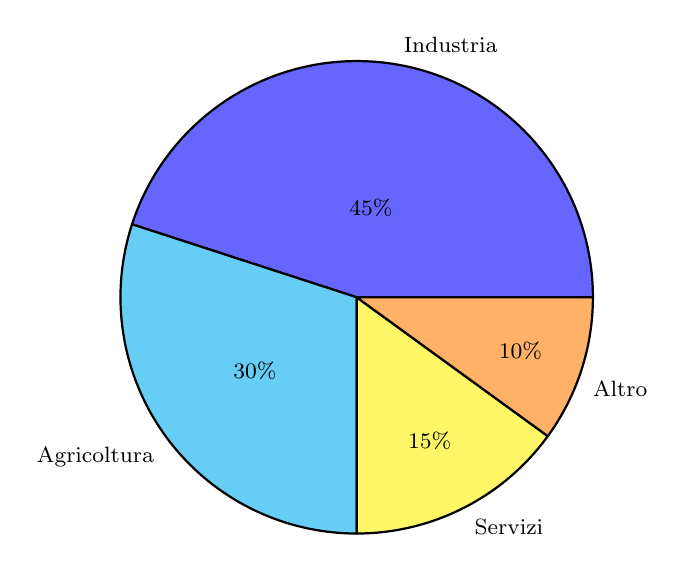
\begin{tikzpicture}
\pie{ 45/Industria, 30/Agricoltura, 15/Servizi, 10/Altro}
\end{tikzpicture}

}


\question
\exonly{
Il seguente grafico riporta la frequenza cumulata nella popolazione maschile. 

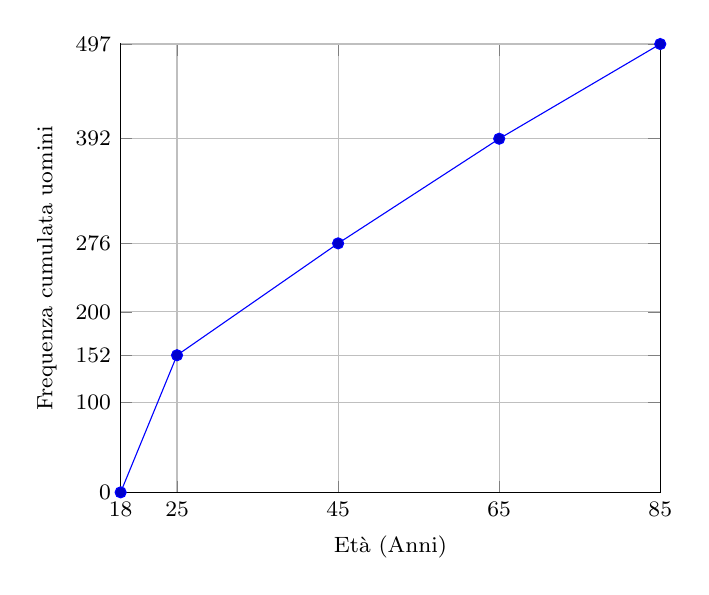
\begin{tikzpicture}
\begin{axis}
[ylabel=Frequenza cumulata uomini,
xlabel=Età (Anni),
enlargelimits=0,
ytick={0,100,200,500,600},
extra y ticks = {152,276,392,497},
ymajorgrids,
xmajorgrids,
minor y tick num=1,
yminorticks=true,
yminorgrids,
xtick={18,25,45,65,85}]
\addplot  coordinates
{ (18,0) (25,152) (45,276) (65,392) (85,497) };
\end{axis}

\end{tikzpicture}

}



\exonly{
Per le donne è data la tabella delle frequenze.

\begin{Tabular}[1.5]{|l|l|l|l|l|}
\hline

Donne &  [18;25[ &  [25;45[ &  [45;65[ &  [65;85[ \\ \hline
Frequenza & 68 & 136 & 105 & 94 \\ \hline

\end{Tabular}
}

\begin{parts}
\part
\exonly{Nel grafico cosa stanno ad indicare i valori 18, 25, 45, ecc.?}
\solonly{I bordi delle classi di età degli uomini della popolazione indagata.}
\part
\exonly{Nel grafico cosa sta ad indicare 152?}
\solonly{152 uomini hanno meno di 25 anni (tra i 18 e i25)}

\part
\exonly{Nel grafico cosa sta ad indicare 276?}
\solonly{276 uomini hanno meno di 45 anni.}

\part
\exonly{Costruire la tabella delle frequenze per gli uomini.}
\solonly{
\begin{Tabular}[1.5]{|l|l|l|l|l|}
\hline

Uomini &  [18;25[ &  [25;45[ &  [45;65[ &  [65;85[ \\ \hline
Frequenza & 152 & 124 & 116 & 105 \\ \hline

\end{Tabular}
}

\part
\exonly{Quante donne compongono la popolazione indagata?}
\solonly{403 donne}

\part
\exonly{In percentuale rispetto alla popolazione totale, quanti uomini compongono la popolazione indagata?}
\solonly{Circa il 55\% della popolazione totale.}

\part\label{ex:perc-uomini}
\exonly{Quanti uomini, in percentuale, rispetto a tutti gli uomini della popolazione hanno meno di 45 anni?}
\solonly{Circa il 56\% degli uomini.}

\part\label{ex:perc-donne}
\exonly{Quante donne, in percentuale, rispetto a tutte le donne della popolazione hanno meno di 45 anni?}
\solonly{Circa il 51 \% delle donne.}

\part\label{ex:perc-tot}
\exonly{Quanti uomini e donne, in percentuale, rispetto a tutta la popolazione hanno meno di 45 anni?}
\solonly{Circa il 53\% della popolazione totale.}

%\part
%\exonly{La media della risposta al punto (\ref{ex:perc-uomini}) e (\ref{ex:perc-donne}) è esattamente uguale al valore trovato al punto (\ref{ex:perc-tot}). Come mai?}
\end{parts}


\exnewpage
\question
\exonly{Il grafico riportato sotto illustra il numero di veicoli immatricolati nel cantone dal 1990 al 2010.
Quale messaggio viene veicolato da questo grafico? Ci sono degli errori? E se si quali?

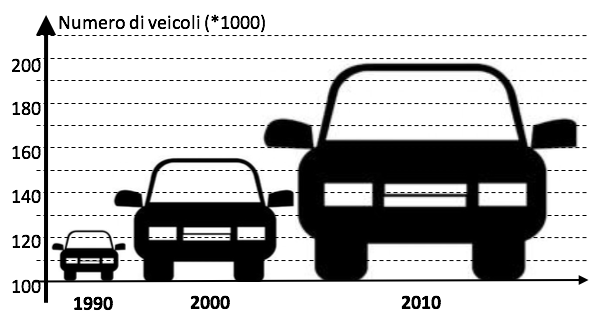
\includegraphics[scale=0.6]{es-grafico-auto}


}
\solonly{Discussione in classe }


\question
\exonly{ 
I due grafici qui sotto rappresentano l’evoluzione del consumo di birra per abitante in Svizzera dal 1981 al 1984.
Quale delle due affermazioni è corretta? Quali elementi del grafico cercano di ingannare il lettore?

\begin{figure}[h!]
\centering
\begin{minipage}{.5\textwidth}
  \centering
  \begin{tikzpicture}
  \begin{axis}[
  AxisDefaults,
  ylabel style={},
  %TinyAxisLabels,
      axis y line=middle, 
      axis x line=bottom,
      xlabel={},
  	ylabel={Consumo [$L/\text{anno}$]},
  xmin=0,
  xmax=3,
  ymin=0,
  ymax=80,
  ytick distance=10,
  xtick={0,1,2,3},
  xticklabels={1981,1982 ,1983 , 1984}
  ]
  \plot[very thick] {-8*x/15+70.2};
  \end{axis}
  \end{tikzpicture}
  \captionof{figure}{Gli Svizzeri bevono sempre tanta birra!}
\end{minipage}%
\begin{minipage}{.5\textwidth}
  \centering
  \begin{tikzpicture}
  \begin{axis}[
  AxisDefaults,
  ylabel style={},
  %TinyAxisLabels,
      axis y line=middle, 
      axis x line=bottom,
      xlabel={},
  	ylabel={Consumo [$L/\text{anno}$]},
  xmin=0,
  xmax=3,
  ymin=68,
  ymax=71,
  ytick distance=0.5,
  xtick={0,1,2,3},
  xticklabels={1981,1982 ,1983 , 1984}
  ]
  \plot[very thick] {-8*x/15+70.2};
  \end{axis}
  \end{tikzpicture}
  \captionof{figure}{Gli Svizzeri bevono meno!}
  \label{fig:test2}
\end{minipage}
\end{figure}


}

\solonly{Discussione in classe }



\question
\exonly{ Data la  distribuzione di una variabile qualitativa nominale (vedi tabella) calcolare le frequenze relative e rappresentare graficamente la distribuzione così ottenuta mediante un grafico a nastri.

\begin{Tabular}[1.5]{|l|l|}
	\hline
	
	 & Freq. assolute cumulative \\ \hline
	A & 25 \\ \hline
	B & 75 \\ \hline
	C & 95 \\ \hline
	D & 100 \\ \hline
	
\end{Tabular}


 }

\solonly{
\begin{tikzpicture}
\begin{axis}[
xbar, xmin=0,
%width=12cm, height=3.5cm, enlarge y limits=-1.5,
xlabel={frequenze in \%},
symbolic y coords={A,B,C,D},
ytick=data,
%nodes near coords, nodes near coords align={horizontal},
]
\addplot coordinates {(25,A) (50,B) (20,C) (5,D)};
\end{axis}
\end{tikzpicture}
 }

\exnewpage
\question
\exonly{
Data la seguente distribuzione relativa ad una variabile continua X:

\begin{Tabular}[1.5]{|l|l|}
	\hline
	
	$X_j$ & Freq. relative  \\ \hline
	$[18;20[$ & 6\% \\ \hline
	$[20;25[$ & 10\% \\ \hline
	$[25;30[$ & 30\% \\ \hline
	$[30; 60[$ & 54\% \\ \hline
	
\end{Tabular}

Stimare la quota di individui con un valore della variabile: 
 }

\begin{parts}
	\part
	\exonly{inferiore a 19  }
	\solonly{3\% }
	\part
	\exonly{superiore a 22 }
	\solonly{90\% }
	\part
	\exonly{compreso fra 40 e 50 }
	\solonly{18\% }
\end{parts}


\question
\exonly{Associare i diagrammi delle frequenze cumulate con i rispettivi istogrammi. 

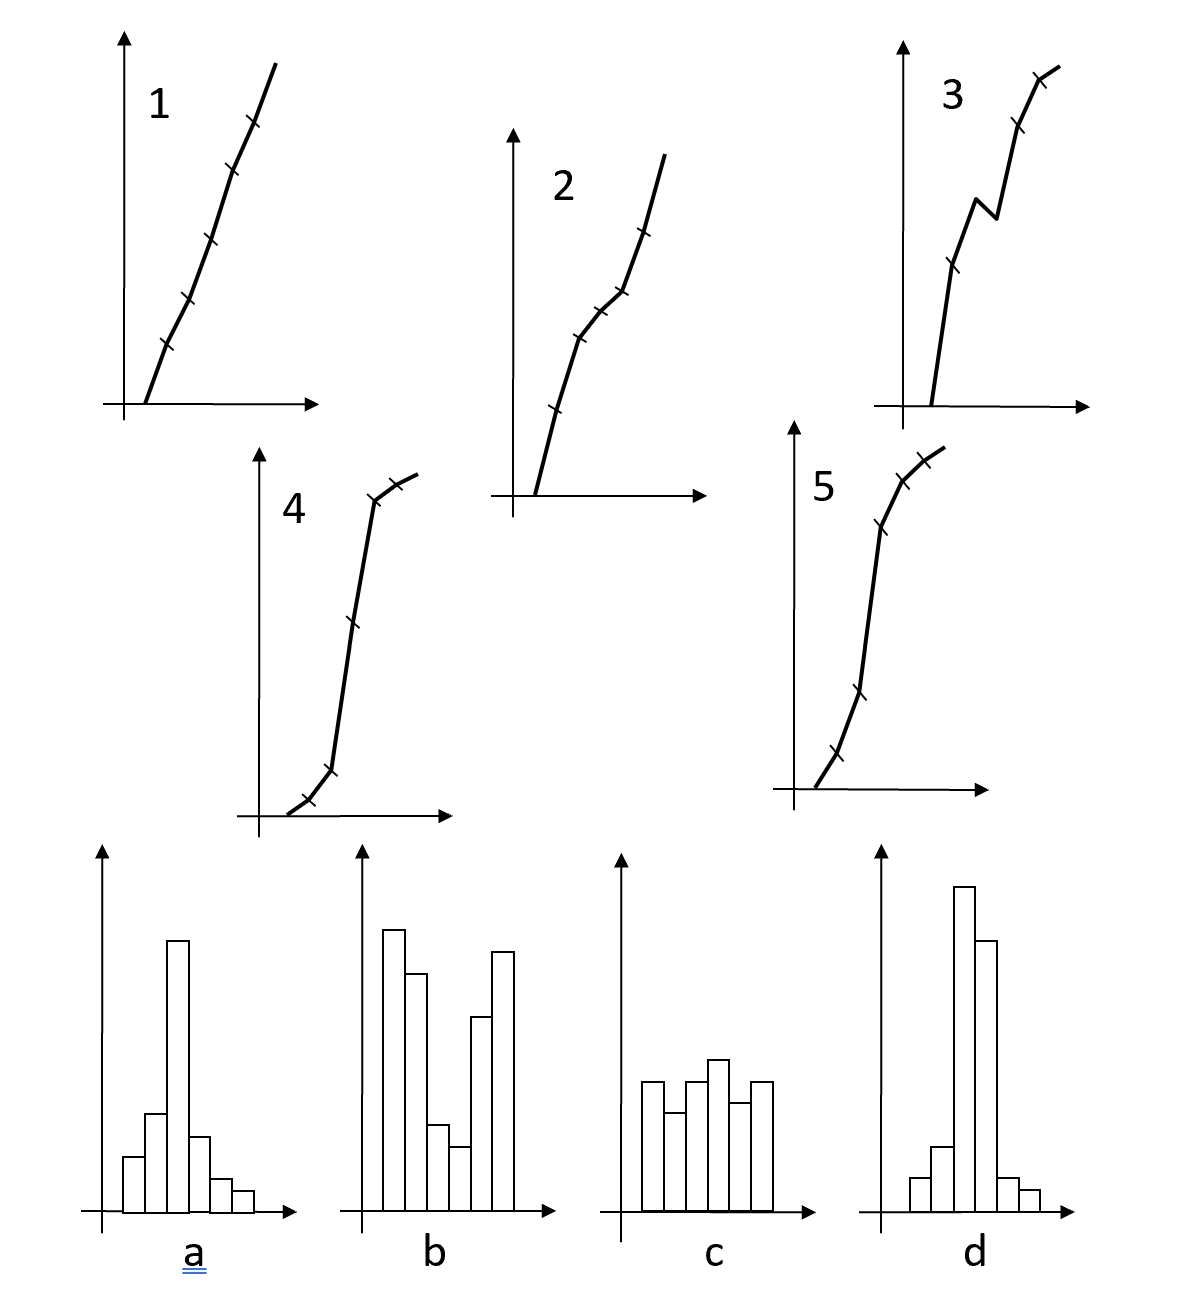
\includegraphics[scale=1]{istogrammma-diagramma_cum}
 }
\solonly{1-c, 2-b, 4-d, 5-a }

\question
\exonly{Data la seguente funzione di ripartizione: 
	
\begin{tikzpicture}
\pgfplotsset{every axis plot post/.append style={ultra thick,mark=none,black}}
\begin{axis}
[ylabel=$F(x)$,
xlabel=$x$,
enlargelimits=0,
ymajorgrids,
ytick distance={0.1},
ymax=1,
%extra y ticks={35,121,245},
xtick={-1,0,1,2,...,4}]
\addplot coordinates {(-1,0) (0,0)};
\addplot coordinates {(0,0.4) (1,0.4)};
\addplot coordinates {(1,0.6) (2,0.6)};
\addplot coordinates {(2,0.9) (3,0.9)};
\addplot coordinates {(3,1) (4,1)};
\end{axis}
\end{tikzpicture}
}

\begin{parts}
	\part 
	\exonly{ Quante sono le modalità? }
	\solonly{5 modalità (-1,0,1,2,3) }
	
	\part
	\exonly{$F(1.5) =$ }
	\solonly{ $F(1.5) = 0.6$   }
	
	\part
	\exonly{Definisci la funzione di ripartizione $F(x)$ }
	\solonly{$F(x) =\begin{cases} 0 & -1 \leq x <0 \\ 0.4 & 0 \leq x <1  \\ 0.6 & 1  \leq x < 2 \\ 0.9 & 2 \leq x <3 \\ 1 & 3 \leq x < 4\end{cases}$}

	\part
	\exonly{Ricostruire la tabella con le frequenze relative e le frequenze relative cumulate. }
	
\end{parts}

\end{questions}

\subsection{Indici di posizione centrale: moda, media, mediana}
\begin{questions}
	\question
	\exonly{Calcola la moda, la media e la mediana di questa distribuzione di frequenza.
	
\begin{Tabular}[1.5]{|l|l|l|l|l|l|l|}
	\hline
	
	$X_j$ & 1 & 2 & 4 & 5 & 6 & 7 \\ \hline
	$n_j$ & 2 & 3 & 5 & 1 & 1 & 2 \\ \hline
	

\end{Tabular} 

}
\solonly{Moda: 4, Media: 3.8 , Mediana: 4 }

\question
\exonly{
	Calcola la moda, la media e la mediana di questa distribuzione di frequenza.

\begin{Tabular}[1.5]{|l|l|l|l|l|l|l|}
	\hline
	
	$X_j$ & 2 & 3 & 4 & 5 & 6 & 7 \\ \hline
	$n_j$ & 3 & 4 & 1 & 5 & 5 & 6 \\ \hline
	
\end{Tabular}
 }
\solonly{Moda: 7, Media: 5 , Mediana: 5 }

\question
\exonly{In un quartiere viene recensito il numero di piani di ogni stabile.

\begin{tabular}{|C{3cm}|C{3cm}|} \hline 
	Numero \newline di piani & Freq. assoluta  \\ \hline\hline 
	1 & 10  \\ \hline 
	2 & 8   \\ \hline 
	3 & 14  \\ \hline 
	4 & 18   \\ \hline 
	5 & 15   \\ \hline 
	6 & 9   \\ \hline \hline
	\textbf{Totale} &    \\ \hline 
\end{tabular}

 }

\begin{parts}
	\part
	\exonly{Calcolare la media di piani degli stabili recensiti }
	\solonly{3.64 piani per stabile }
	\part
	\exonly{Calcolare la media di piani se ai dati iniziali aggiungiamo 3 immobili di 16 piani }
	\solonly{4.12 piani per stabile }
	\part
	\exonly{ Calcolare la media di piani se ai dati iniziali aggiungiamo 10 case  di 1 piano  }
	\solonly{3.32 piani per stabile }
	\part
	\exonly{Calcolare la media di piani se, sempre partendo dai dati iniziali, alzassimo 8 stabili di 1 piano. }
	\solonly{3.74 piani per stabile }
\end{parts}

\question
\exonly{ Determinare le tre misure di tendenza centrale di questa statistica che concerne il numero di impiegati di alcune piccole imprese.

\begin{Tabular}[1.5]{|C{3cm}|C{3cm}|C{3cm}|C{3cm}|} \hline 
	Numero di impiegati & Freq. assoluta &  &  \\ \hline\hline 
	1 & 22 &  &  \\ \hline 
	2 & 41 &  &  \\ \hline 
	3 & 55 &  &  \\ \hline 
	4 & 86 &  &  \\ \hline 
	5 & 108 &  &  \\ \hline 
	6 & 75 &  &  \\ \hline 
	7 & 42 &  &  \\ \hline 
	8 & 25 &  &  \\ \hline \hline
	\textbf{TOT} &  &  &  \\ \hline 
\end{Tabular}
 }
\solonly{Moda 5 , Media $4.62$ , Mediana $5$ }

\question
\exonly{Determinare le tre misure di tendenza centrale di questa statistica che concerne la superficie degli appartamenti abitativi di un quartiere.

\begin{Tabular}[1.5]{|C{3cm}|C{3cm}|C{3cm}|C{3cm}|C{3cm}|} \hline
	Superficie (in m${}^{2}$) & Freq. assoluta &  &  &  \\ \hline\hline 
	[0;20[ & 15 &  &  &  \\ \hline 
	[20;40[ & 18 &  &  &  \\ \hline 
	[40;60[ & 28 &  &  &  \\ \hline 
	[60;80[ & 51 &  &  &  \\ \hline 
	[80;100[ & 32 &  &  &  \\ \hline 
	[100;120[ & 19 &  &  &  \\ \hline \hline
	\textbf{TOT.} &  &  &  &  \\ \hline 
\end{Tabular}

 }
\solonly{Moda $[60;80[$ , Media $65.21$ , Mediana $68.04$ }
\end{questions}

\exnewpage

\subsection{Misure di dispersione: quartili, scarto quadratico medio}

\begin{questions}
		\question
	\exonly{
		Associare gli istogrammi ai boxplot corrispondenti.
		
		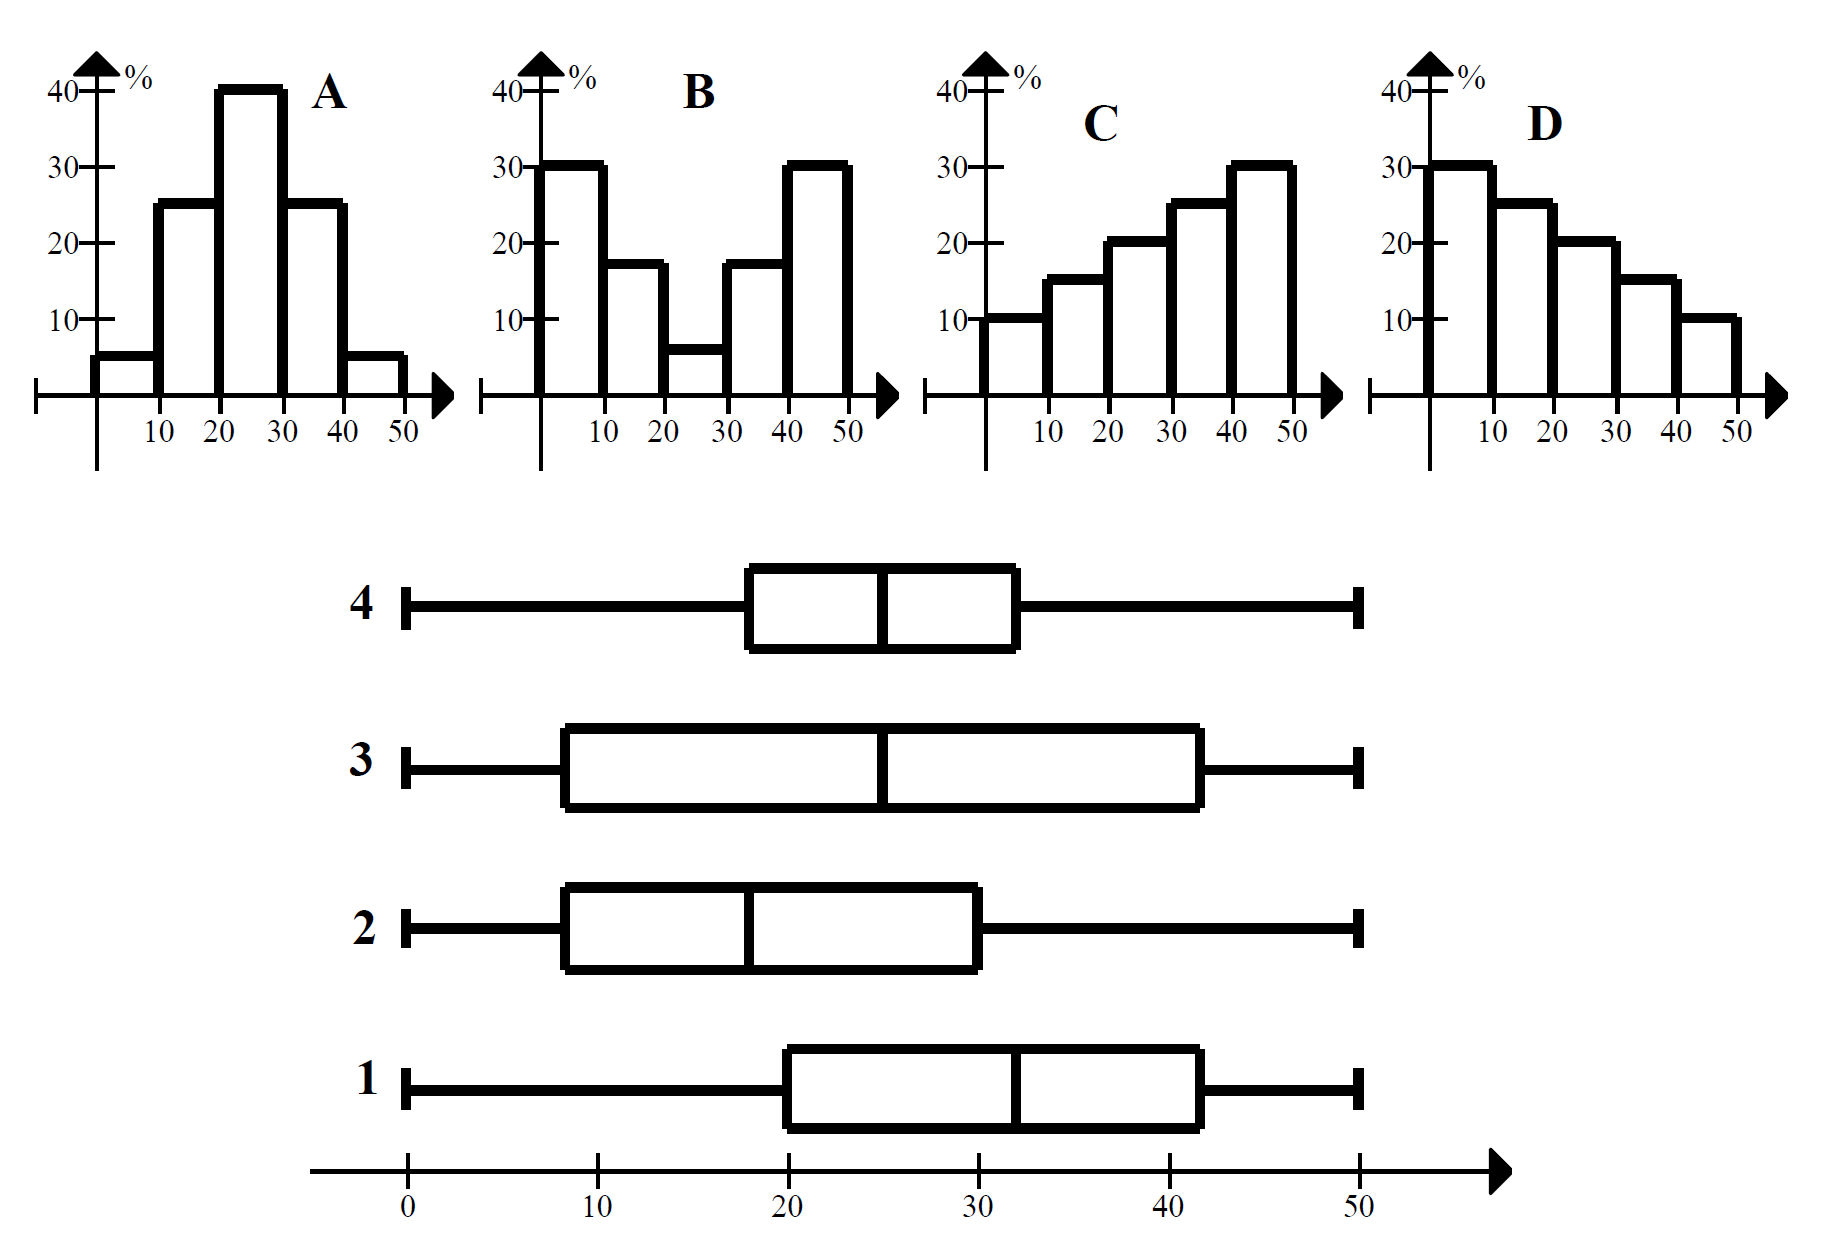
\includegraphics[scale=0.6]{istogrammi-boxplot} }
	\exonly{Discussione in classe }
	\question
	\exonly{
		Il servizio clienti di una grande ditta registra il numero di mail ai quali i suoi impiegati hanno risposto in un ora. I risultati sono sintetizzati nel boxplot qui sotto.
		
		\begin{tikzpicture}
		\begin{axis}
		[
		height=3cm,
		width=9cm,
		hide y axis,
		axis x line*=bottom,
		xtick distance=1,
		]
		
		\addplot+[
		boxplot prepared={
			median=8,
			upper quartile=14,
			lower quartile=5,
			upper whisker=18,
			lower whisker=2
		},
		] coordinates {};
		\end{axis}
		\end{tikzpicture}
	}
	
	\begin{parts}
		\part
		\exonly{Determinare i tre quartili della statistica e lo scarto interquartile. Interpretare i dati. }
		\solonly{$Q_1=5$ , $Q_2=8$ , $Q_3=14$ , scarto: $9$ }
		
		\part
		\exonly{ L'impiegato che ha risposto al minor numero di mail quanti ne ha trattati? E quello che ne ha trattai il maggior numero?  }
		\solonly{Minimo: 2, Massimo : 18 }
		
		\part
		\exonly{Che percentuale degli impiegati ha trattato 8 mail o più? }
		\solonly{50\% }
		
		\part
		\exonly{Che percentuale degli impiegati ha trattato tra i 5 e 14 mail? }
		\solonly{50\% }
		
		\part
		\exonly{Il quarto degli impiegati che ha risposto a meno casi quanti ne ha trattati ? }
		\solonly{Meno di 5 }
	\end{parts}

\question
\exonly{
	Ecco i risultati di 24 allievi per un esame (numero di punti massimi 100).

\begin{tabular}{llllllll}
	78 & 79 & 77 & 59 & 57 & 65 & 65 & 67 \\ 
	68 & 67 & 59 & 54 & 64 & 68 & 72 & 74 \\ 
	72 & 72 & 76 & 77 & 76 & 74 & 77 & 76 \\ 
\end{tabular}

 }

\begin{parts}
	\part
	\exonly{Determinare la mediana e i quartili di questa serie. }
	\solonly{Mediana: 72, $Q_1=65$, $Q_3=76$ }
	\part
	\exonly{Disegnare il boxplot }
	\solonly{
		\begin{tikzpicture}
	\begin{axis}
	[
	height=3cm,
	width=9cm,
	hide y axis,
	axis x line*=bottom,
	xtick distance=2,
	]
	
	\addplot+[
	boxplot prepared={
		median=72,
		upper quartile=76,
		lower quartile=65,
		upper whisker=79,
		lower whisker=54
	},
	] coordinates {};
	\end{axis}
	\end{tikzpicture}
 }

\part
\exonly{
Si possono comparare i risultati di questa classe con quelli di un'altra classe.

 Della seconda classe si sa che: le due note più basse sono 47 e 55 , la nota massima è 85, la mediana 70, Q1=67 e Q3=76. 
 
 Tracciare sullo stesso grafico anche questo boxplot e comparare le due classi.
 }

\solonly{
	\begin{tikzpicture}
\begin{axis}
[
height=3cm,
width=9cm,
hide y axis,
axis x line*=bottom,
xtick distance=2,
]

\addplot+[
boxplot prepared={
	median=72,
	upper quartile=76,
	lower quartile=65,
	upper whisker=79,
	lower whisker=54
},
] coordinates {};
\addplot+[
boxplot prepared={
	median=70,
	upper quartile=76,
	lower quartile=67,
	upper whisker=85,
	lower whisker=55
},
] coordinates {(0,47)};
\end{axis}
\end{tikzpicture}

 }
\end{parts}

\question
\exonly{
	La rappresentazione grafica seguente raffigura l'evoluzione del tasso di mortalità infantile (mortalità infantile per 1000 nascite in vita) dal 1901 al 1975 in Svizzera (dati dei 25 Cantoni).
	
	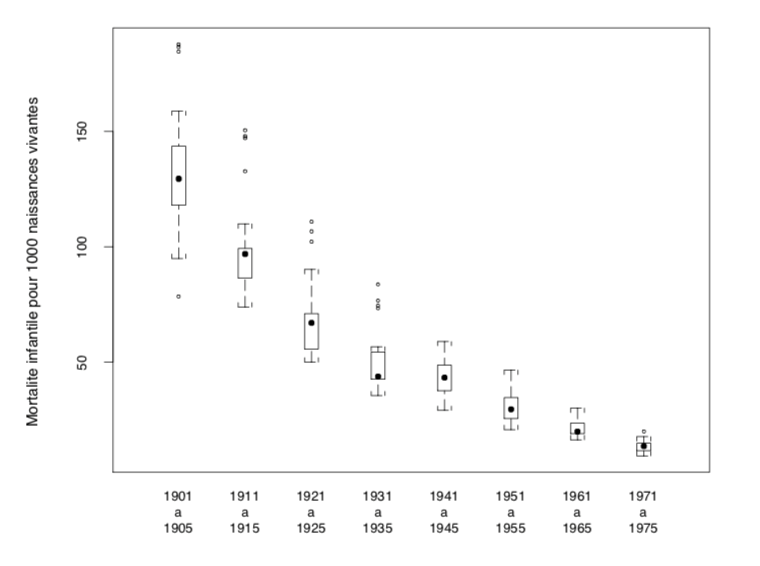
\includegraphics[scale=0.8]{box-plot-nascite}
	
Come interpretare le informazioni seguenti :
\begin{parts}
	\part I box sono sempre più piccoli 
	\part I box sono sempre più in basso
	\part Nel 1921 il baffo superiore è molto più grande di quello inferiore
	\part  In quale periodo la maggior parte dei cantoni aveva un tasso di mortalità  inferiore alla mediana? 
	\part I dati sono raggruppati su periodi di 5 anni e non di un anno? 
	\part Perché 25 cantoni e non 26? 
\end{parts} 
}

\solonly{Discussione in classe }
	
	\question
	
\exonly{Calcola media aritmetica, moda, mediana e scarto quadratico medio della seguente distribuzione di frequenza. 

\begin{Tabular}{|l|l|l|l|l|l|}
	\hline
	
	$X_j$ & 1 & 3 & 4 & 5 & 11 \\ \hline
	$n_j$ & 1 & 3 & 1 & 4 & 1 \\ \hline
	
\end{Tabular}
}

\solonly{Media: $\overline{x}=4.5$ e $\sigma=2.5$ , Moda: 5, Mediana: $\tilde{x}=4.5$}

 	\question
 	\exonly{
 	Calcola media aritmetica, moda, mediana e scarto quadratico medio della seguente distribuzione di frequenza. 
 

	\begin{Tabular}[1.5]{|l|l|l|l|l|}
		\hline
		
		$X_j$ & 1,4 & 2,4 & 3,4 & 4,4 \\ \hline
		$n_j$ & 1 & 1 & 1 & 4 \\ \hline
		
	\end{Tabular}
	 }
 	\solonly{Media: $\overline{x}=3.54$ e $\sigma=1.13$ , Moda: 4.4, Mediana: $\tilde{x}=4.4$}
 	
 	\exnewpage
 	\question
 	\exonly{
 	Sapendo che la distribuzione di frequenza 
 	
 	\begin{Tabular}[1.5]{|l|l|l|l|l|}
 		\hline
 		
 		$X_j$ & 5 & 10 & 15 & 20 \\ \hline
 		$n_j$ & \cellcolor[gray]{.9} $n_1$ & 3 & 1 & 1 \\ \hline
 		
 	\end{Tabular}

	ha media aritmetica $\overline{x}=9$, ricostruisci la frequenza mancante.
		 }
	 \solonly{$n_1=5$ }
 	
 	
	\question
	\exonly{Nell'ambito di un controllo di qualità (scegliendo un campione di lotti prodotti) si é notato il numero di pezzi difettati di ogni lotto esaminato.
	
\begin{tikzpicture}
\begin{axis}[
xlabel = Quantità di pezzi difettati costatati,
xtick={1,...,7},
ytick={0,5,10,...,90},
grid=major,
%minor y tick num=1,
%x tick label style={rotate=45,anchor=east},
ylabel=Frequenza (Numero di lotti),
enlargelimits=0.05,
%legend style={at={(0.5,-0.15)}, anchor=north,legend columns=-1},
ybar interval=0.3,
%xticklabel shift={.3cm},
%xticklabel=[\pgfmathprintnumber\tick;\pgfmathprintnumber\nexttick [
]
\addplot coordinates
{(0,85) (1,25) (2,35) (3,60) (4,25) (5,15) (6,10) (7,0)};
\end{axis}
\end{tikzpicture}

 }


\exonly{Calcolare la media e lo scarto quadratico medio di pezzi difettati per lotto. Se siamo disposto a tollerare un massimo di 2 pezzi difettosi per lotto acquisteremmo da questo fabbricante? E se ne tollerassimo 3? Oppure 4?  }

\solonly{ $\bar{x}=2$ $\sigma=1.8$. Quindi maggioranza dei dati tra $[0;3]$.
	
	In generale avremo tra gli 0 i 3 pezzi difettosi in un lotto, quindi non acquisteremmo se tolleriamo al massimo 2 pezzi difettosi (molto spesso ce ne sono 3). Potremmo acquistare se ne tolleriamo 3 ma nel 15\% ca. dei casi potremmo averne 4. Se ne tollerassimo 4 acquisteremmo perché solo nel 2.5\% ca. dei casi i pezzi difettati saranno più di 4}


\question
\exonly{Determinare la media e lo scarto quadratico medio di questa statistica che si interessa alla durata delle telefonate di una classe della vostra scuola in una settimana 

\begin{Tabular}[1.5]{|C{2cm}|C{2cm}|C{2cm}|C{2cm}|C{2cm}|C{2cm}|} \hline 
	Durata della telefonata \newline (secondi) & Frequenza \newline assoluta  &  &  &    & \\ \hline \hline 
	[0;30[ & 45 &  &  &  &  \\ \hline 
	[30;60[ & 48 &  &  &  &  \\ \hline 
	[60;90[ & 77 &  &  &  &  \\ \hline 
	[90;120[ & 124 &  &  &  &  \\ \hline 
	[120;150[ & 88 &  &  &  &  \\ \hline 
	[150;180[ & 64 &  &  &  &  \\ \hline \hline 
	\textbf{TOT.} & 446 &  &  &  &  \\ \hline 
\end{Tabular}

}
\solonly{$\bar{x}= 98.81$ e $ \sigma=44.9$}

% 	\question
%\exonly{
%	Sapendo che la distribuzione di frequenza 
%	
%	\begin{Tabular}[1.5]{|l|l|l|l|l|}
%		\hline
%		
%		$X_j$ & 1 & 1.5 & 2 & 2.5 \\ \hline
%		$n_j$ & 4 & 1 & 2 & \cellcolor[gray]{.9} $n_4$ \\ \hline
%		
%	\end{Tabular}
%	
%	ha varianza $\sigma ^2=0.41$, ricostruisci la frequenza mancante.
%}
%\solonly{$n_4=$ }
\end{questions}



%\subsection{Esercizi ricapitolativi}

\end{document}